\documentclass[english, 12pt, a4paper, elec, utf8, a-2b, online]{aaltothesis}
%\documentclass[english, 12pt, a4paper, elec, utf8, a-2b, print]{aaltothesis}
%\documentclass[english, 12pt, a4paper, elec, utf8, a-2b, print, twoside]{aaltothesis}

\setupthesisfonts

% Language setting
% Replace `english' with e.g. `spanish' to change the document language
% \usepackage[english]{babel}
\usepackage{float}

% Set page size and margins
% Replace `letterpaper' with `a4paper' for UK/EU standard size
% \usepackage[letterpaper,top=2cm,bottom=2cm,left=3cm,right=3cm,marginparwidth=1.75cm]{geometry}

% Useful packages
\usepackage{amsmath, amssymb}
\usepackage{amsmath}
\usepackage{graphicx}
% \usepackage{algorithm}
\usepackage[ruled,vlined]{algorithm2e}
% \usepackage{algorithmic}
% \usepackage{algpseudocode}
% \usepackage[colorlinks=true, allcolors=blue]{hyperref}
\usepackage{longtable}
\usepackage[type={CC}, modifier={by-nc-sa}, version={4.0}]{doclicense}

\degreeprogram{Electronics and Electrical Engineering}

\title{Hierarchical Reinforcement Learning with Finite State Machines for Multi-Robot Collaborative Manipulation}
\author{Yutong Du}

\begin{document}
\maketitle

\begin{abstract}
1 - In a Multi-Robot collaborative scenario, adding a new robot brings additional development work.
2 - This work proposed a new algorithm that includes observing and learning the working pattern of the main robot and accelerating task completion with more robots manipulated by reinforcement learning models.
3 - 

\end{abstract}

% \section{Introduction}

% Your introduction goes here! Simply start writing your document and use the Recompile button to view the updated PDF preview. Examples of commonly used commands and features are listed below, to help you get started.

% Once you're familiar with the editor, you can find various project settings in the Overleaf menu, accessed via the button in the very top left of the editor. To view tutorials, user guides, and further documentation, please visit our \href{https://www.overleaf.com/learn}{help library}, or head to our plans page to \href{https://www.overleaf.com/user/subscription/plans}{choose your plan}.

% \section{Some examples to get started}

% \subsection{How to create Sections and Subsections}

% Simply use the section and subsection commands, as in this example document! With Overleaf, all the formatting and numbering is handled automatically according to the template you've chosen. If you're using the Visual Editor, you can also create new section and subsections via the buttons in the editor toolbar.

% \subsection{How to include Figures}

% First you have to upload the image file from your computer using the upload link in the file-tree menu. Then use the includegraphics command to include it in your document. Use the figure environment and the caption command to add a number and a caption to your figure. See the code for Figure \ref{fig:frog} in this section for an example.

% Note that your figure will automatically be placed in the most appropriate place for it, given the surrounding text and taking into account other figures or tables that may be close by. You can find out more about adding images to your documents in this help article on \href{https://www.overleaf.com/learn/how-to/Including_images_on_Overleaf}{including images on Overleaf}.

% \begin{figure}
% \centering
% \includegraphics[width=0.25\linewidth]{frog.jpg}
% \caption{\label{fig:frog}This frog was uploaded via the file-tree menu.}
% \end{figure}

% \subsection{How to add Tables}

% Use the table and tabular environments for basic tables --- see Table~\ref{tab:widgets}, for example. For more information, please see this help article on \href{https://www.overleaf.com/learn/latex/tables}{tables}.

% \begin{table}
% \centering
% \begin{tabular}{l|r}
% Item & Quantity \\\hline
% Widgets & 42 \\
% Gadgets & 13
% \end{tabular}
% \caption{\label{tab:widgets}An example table.}
% \end{table}

% \subsection{How to add Comments and Track Changes}

% Comments can be added to your project by highlighting some text and clicking ``Add comment'' in the top right of the editor pane. To view existing comments, click on the Review menu in the toolbar above. To reply to a comment, click on the Reply button in the lower right corner of the comment. You can close the Review pane by clicking its name on the toolbar when you're done reviewing for the time being.

% Track changes are available on all our \href{https://www.overleaf.com/user/subscription/plans}{premium plans}, and can be toggled on or off using the option at the top of the Review pane. Track changes allow you to keep track of every change made to the document, along with the person making the change.

% \subsection{How to add Lists}

% You can make lists with automatic numbering \dots

% \begin{enumerate}
% \item Like this,
% \item and like this.
% \end{enumerate}
% \dots or bullet points \dots
% \begin{itemize}
% \item Like this,
% \item and like this.
% \end{itemize}

% \subsection{How to write Mathematics}

% \LaTeX{} is great at typesetting mathematics. Let $X_1, X_2, \ldots, X_n$ be a sequence of independent and identically distributed random variables with $\text{E}[X_i] = \mu$ and $\text{Var}[X_i] = \sigma^2 < \infty$, and let
% \[S_n = \frac{X_1 + X_2 + \cdots + X_n}{n}
%       = \frac{1}{n}\sum_{i}^{n} X_i\]
% denote their mean. Then as $n$ approaches infinity, the random variables $\sqrt{n}(S_n - \mu)$ converge in distribution to a normal $\mathcal{N}(0, \sigma^2)$.


% \subsection{How to change the margins and paper size}

% Usually the template you're using will have the page margins and paper size set correctly for that use-case. For example, if you're using a journal article template provided by the journal publisher, that template will be formatted according to their requirements. In these cases, it's best not to alter the margins directly.

% If however you're using a more general template, such as this one, and would like to alter the margins, a common way to do so is via the geometry package. You can find the geometry package loaded in the preamble at the top of this example file, and if you'd like to learn more about how to adjust the settings, please visit this help article on \href{https://www.overleaf.com/learn/latex/page_size_and_margins}{page size and margins}.

% \subsection{How to change the document language and spell check settings}

% Overleaf supports many different languages, including multiple different languages within one document.

% To configure the document language, simply edit the option provided to the babel package in the preamble at the top of this example project. To learn more about the different options, please visit this help article on \href{https://www.overleaf.com/learn/latex/International_language_support}{international language support}.

% To change the spell check language, simply open the Overleaf menu at the top left of the editor window, scroll down to the spell check setting, and adjust accordingly.

% \subsection{How to add Citations and a References List}

% You can simply upload a \verb|.bib| file containing your BibTeX entries, created with a tool such as JabRef. You can then cite entries from it, like this: \cite{gree93}. Just remember to specify a bibliography style, as well as the filename of the \verb|.bib|. You can find a \href{https://www.overleaf.com/help/97-how-to-include-a-bibliography-using-bibtex}{video tutorial here} to learn more about BibTeX.

% If you have an \href{https://www.overleaf.com/user/subscription/plans}{upgraded account}, you can also import your Mendeley or Zotero library directly as a \verb|.bib| file, via the upload menu in the file-tree.

% \subsection{Good luck!}

\section{Literature Review}

\paragraph{Overview of Reinforcement Learning in Robotics.}
Reinforcement learning (RL) has emerged as a cornerstone framework for sequential decision-making in robotics, offering a principled approach to learning control policies through trial-and-error interaction with dynamic environments. By formalizing the learning problem as a Markov Decision Process (MDP), RL enables an agent to reason about the long-term consequences of its actions through state transitions, probabilistic dynamics, and reward feedback. This formulation allows robots to autonomously acquire adaptive behaviors for navigation, manipulation, and coordination without the need for explicit motion planning or hand-crafted control laws. The integration of MDPs with deep neural networks, particularly multilayer perceptrons (MLPs), has further enhanced the capacity of RL systems to handle high-dimensional continuous control tasks, making it a powerful paradigm for intelligent robotic systems operating in complex and uncertain environments.



\subsection{Reinforcement Learning for Robotic Navigation and Manipulation}

Reinforcement learning (RL) has become a powerful framework for developing autonomous robotic control systems capable of learning complex behaviors directly from interaction with the environment. By modeling robotic control as a sequential decision-making problem, RL enables robots to acquire navigation, manipulation, and coordination skills without relying on explicit motion planning or manual trajectory design.

\paragraph{Robot Navigation Control.}
In the domain of robot navigation, RL has been widely used to train mobile agents capable of obstacle avoidance, goal-oriented movement, and path optimization in dynamic environments. Early works demonstrated the feasibility of using model-free algorithms such as Deep Q-Networks (DQN) \cite{mnih2015human} and policy-gradient-based methods like Proximal Policy Optimization (PPO) \cite{schulman2017proximal} to learn end-to-end navigation policies. For instance, Tai et al. \cite{tai2017virtual} trained differential-drive robots for autonomous navigation using continuous control RL, achieving robust path-following behavior in simulation. Similarly, Zhu et al. \cite{zhu2017target} employed visual RL for target-driven navigation, allowing agents to interpret camera inputs to reach designated goals. These studies often leverage simulation platforms such as MuJoCo \cite{todorov2012mujoco} or OpenAI Gym \cite{brockman2016openai} to model the physics-based interactions required for realistic robotic locomotion. More recent research, such as \cite{9351818}, further integrates RL with hierarchical or graph-based planners, improving generalization to large-scale and partially observable navigation environments.

\paragraph{Robotic Arm Control for Grasping and Placement.}
Beyond navigation, RL has also been successfully applied to robotic manipulation, including grasping, pick-and-place, and high-precision assembly tasks. Levine et al. \cite{levine2018learning} and Kalashnikov et al. \cite{kalashnikov2018qt} proposed end-to-end visuomotor learning frameworks, where policies are trained to directly map raw image inputs to continuous motor torques. Haarnoja et al. \cite{haarnoja2018soft} introduced the Soft Actor-Critic (SAC) algorithm, which achieved stable and sample-efficient learning in continuous action spaces—making it particularly suitable for robotic arms. Other works, such as Mahler et al. \cite{mahler2019learning}, applied deep RL to dexterous grasping by combining simulation-based training with real-world fine-tuning. Zeng et al. \cite{zeng2020tossingbot} further extended this idea to dynamic placement tasks, where a robot learned to grasp and throw objects with accurate control of release timing and velocity. These studies commonly employ standard robotic models provided in the MuJoCo Model Gallery—most notably the \textit{Franka Emika Panda} and \textit{Universal Robots UR5/UR10}—which serve as canonical benchmarks for manipulation research due to their stable dynamics and open-source availability.

\paragraph{Research Gap and Motivation.}
Despite these advancements, most existing works address either navigation or manipulation in isolation. RL-based navigation research typically focuses on mobile robots without manipulation capability, while RL-based manipulation studies assume a fixed-base robotic arm operating in a static workspace. In contrast, many practical industrial and logistics applications—such as warehouse automation and material handling—require an integrated system combining both mobility and dexterous manipulation, such as automated guided vehicles (AGVs) equipped with robotic arms. This configuration introduces additional challenges related to non-stationary dynamics, joint optimization of navigation and manipulation policies, and inter-agent coordination within the same control framework. 

Moreover, prior simulation studies have been limited to standard robotic arm models (e.g., Franka, UR5) with conventional two-finger or parallel-jaw grippers. Few have investigated lightweight or educational robotic arms such as the \textit{WLKATA Mirobot}, particularly those equipped with suction-based end-effectors, which involve distinct contact mechanics and pneumatic dynamics. Given that the target hardware platform in our laboratory integrates a WLKATA robotic arm mounted on an AGV, existing research provides insufficient insight into sim-to-real transfer for such systems. Addressing this gap is essential for developing robust RL-based control policies capable of handling mobile manipulation tasks in dynamic, physics-consistent environments.


Simulated environments, such as MuJoCo \cite{todorov2012mujoco} and OpenAI Gym \cite{brockman2016openai}, have played a crucial role in facilitating the development of RL-based robotic controllers. By providing accurate modeling of rigid-body dynamics, collision detection, and contact forces, these simulators allow for safe and efficient policy training without the risks associated with real-world experimentation. Moreover, parallel environment execution and reproducible training pipelines, often supported by frameworks such as Stable-Baselines3 (SB3) \cite{raffin2021stable}, accelerate the convergence of RL policies and facilitate systematic hyperparameter tuning.

\subsection{Multi-Agent and Collaborative Reinforcement Learning}

\paragraph{Extension of Reinforcement Learning to Multi-Agent Systems.}
Building upon the success of single-agent reinforcement learning, the multi-agent reinforcement learning (MARL) framework extends the Markov Decision Process (MDP) to accommodate multiple interacting agents, each optimizing its own policy while considering the influence of others \cite{zhang2021multi}. This paradigm enables the modeling of cooperative, competitive, and mixed-agent scenarios, making it particularly relevant for multi-robot systems that operate in shared workspaces. The fundamental objective in MARL is to balance individual decision-making and collective performance, often requiring the development of coordination mechanisms and joint policy optimization strategies.

\paragraph{Dominance of Discrete and Grid-Based Environments.}
Despite its theoretical richness, most MARL research has been conducted in discrete and grid-structured domains such as the Atari benchmark \cite{mnih2015human} and cooperative environments like Overcooked \cite{carroll2019utility}. In these settings, agents navigate a limited number of discrete states and actions, typically on a 2D grid, which simplifies reward propagation and state transitions. However, such discrete abstractions do not accurately represent the continuous, dynamic, and high-dimensional nature of robotic control tasks. In real-world robotic environments—such as those simulated in MuJoCo—agents must reason over continuous state-action spaces, handle dynamic physical interactions, and adapt to sensor noise and uncertainty \cite{iqbal2019actor, mahajan2019maven}. This fundamental difference limits the applicability of grid-based MARL research to realistic robotic systems.

\paragraph{Centralized Coordination and Scalability Limitations.}
A large body of MARL literature relies on centralized or semi-centralized coordination frameworks. The Centralized Training with Decentralized Execution (CTDE) paradigm \cite{lowe2017multi} allows agents to share global information during training while executing policies independently at runtime. Other approaches, such as QMIX \cite{rashid2020monotonic} and parameter sharing among homogeneous agents \cite{gupta2017cooperative}, have been proposed to improve stability and sample efficiency. Nevertheless, these frameworks inherently limit scalability and autonomy, as they depend on centralized critics or tightly coupled parameter structures. Consequently, they struggle in industrial scenarios where robots may need to operate independently or in small cooperative groups without centralized control or high-bandwidth communication.

\paragraph{Emergence of Decentralized and Scalable MARL Frameworks.}
To address these limitations, recent research has shifted toward decentralized and scalable MARL approaches, enabling each agent to maintain its own policy while still achieving emergent cooperation through shared objectives or local communication \cite{foerster2018counterfactual}. Such frameworks are particularly suitable for industrial contexts where autonomy, fault tolerance, and modularity are essential. In decentralized policy gradient methods, each agent optimizes its parameters independently using local observations, while coordination emerges implicitly through environmental feedback. This design philosophy aligns closely with the principles of Industry~5.0, emphasizing human–robot collaboration, adaptability, and flexible automation across distributed robotic systems.

\paragraph{Research Gap and Motivation.}
Although MARL has achieved remarkable progress in simulated and discrete domains, its application to continuous, physics-based industrial settings remains limited. Existing works typically focus either on multi-robot navigation or on collaborative manipulation, but rarely on integrated systems that combine mobile platforms and robotic arms. Furthermore, most prior studies rely on standard MuJoCo models such as Franka Emika Panda or Universal Robots, leaving lightweight, educational platforms—such as the WLkata robotic arm equipped with a vacuum-based end-effector—largely unexplored. As future robotic systems evolve toward adaptive and scalable autonomy, there is a pressing need for decentralized reinforcement learning frameworks capable of controlling AGV-mounted manipulators that can operate both independently and collaboratively. This research aims to address this gap by developing a scalable, decentralized MARL-based control system for real-world industrial robotics and advancing the sim-to-real transition for flexible automation.


\subsection{Summary of Trends and Open Challenges}

\paragraph{Trends in Reinforcement Learning for Robotics.}
The recent literature reveals several converging trends in the application of RL to robotic control. First, MDP-based formulations combined with deep neural network policies—most notably Proximal Policy Optimization (PPO) and Soft Actor-Critic (SAC)—have become the dominant paradigm for learning robust control strategies in both discrete and continuous domains. These methods allow robots to generalize across varied environments while maintaining sample efficiency and stability during training. Second, simulation environments such as MuJoCo \cite{todorov2012mujoco}, OpenAI Gym \cite{brockman2016openai}, and advanced toolkits like Stable-Baselines3 (SB3) \cite{raffin2021stable} have become indispensable for policy development, enabling reproducible, physics-consistent experimentation before real-world deployment. Third, within multi-agent reinforcement learning (MARL), frameworks such as Centralized Training with Decentralized Execution (CTDE) \cite{lowe2017multi} and parameter sharing \cite{gupta2017cooperative} have demonstrated scalable cooperation across homogeneous agents, marking a significant step toward coordinated robotic systems.

\paragraph{Persistent Challenges and Research Gaps.}
Despite these advances, several fundamental challenges persist. Sim-to-real transfer remains a major obstacle due to discrepancies between simulated and real-world physics, sensor noise, and actuator latency. Furthermore, most MARL research continues to rely on discrete, grid-based benchmarks (e.g., Atari, Overcooked) that fail to capture the continuous, high-dimensional, and physics-driven nature of industrial robotic environments. The dependence on centralized critics or global communication during training also limits the scalability and autonomy of learned policies, making them unsuitable for decentralized robotic systems operating in dynamic industrial settings.

Another critical gap lies in the lack of research addressing integrated mobile manipulation systems, where a robotic arm is mounted on a mobile platform such as an Automated Guided Vehicle (AGV). Existing studies predominantly focus on either navigation or manipulation in isolation, leaving the joint control of mobility and dexterity largely unexplored. Additionally, lightweight and educational robotic platforms—such as the \textit{WLKATA Mirobot} equipped with suction-based end-effectors—remain underrepresented in RL research despite their potential for scalable, cost-effective experimentation. 

\paragraph{Motivation for the Present Study.}
In the context of Industry~5.0, where autonomy, flexibility, and human–robot collaboration are central, there is a growing demand for decentralized and scalable reinforcement learning frameworks capable of enabling heterogeneous robots to operate both independently and collaboratively. This study is motivated by the need to bridge the gap between simulated continuous-control MARL and real-world robotic systems. Specifically, it seeks to develop and evaluate a decentralized MDP-based RL framework using PPO-trained MLP policies for AGV-mounted robotic manipulators. By focusing on scalable policy architectures and transferable learning strategies, the present work aims to contribute to the broader goal of achieving adaptive, cooperative, and physics-consistent robotic control in next-generation industrial environments.

\section{Materials and Methods}

\subsection{Simulation Platform and Experimental Setup}

The simulation environment was developed using the \textbf{MuJoCo} physics engine, which enables precise modeling of rigid-body dynamics, collision detection, and contact interactions. The environment includes the following components:
\begin{itemize}
    \item Boundary walls and a floor defining the workspace;
    \item Multiple objects available for picking and placing;
    \item Four designated placement plates and two picking tables for task execution;
    \item Multiple six-degree-of-freedom robotic arms mounted on automated guided vehicles (AGVs) of the same type.

\end{itemize}


The experiments were executed on a workstation with the following configuration: Intel Core i9 CPU, 64~GB RAM, running Ubuntu~22.04 LTS (WSL2). Python~3.11 was used as the programming language. 

For reinforcement learning, we employed \textbf{Stable-Baselines3 (SB3)}, a Python package providing modular and reliable implementations of state-of-the-art RL algorithms, including Proximal Policy Optimization (PPO). SB3 supports parallel environment execution, automatic logging, and reproducible training pipelines, facilitating efficient policy optimization in high-dimensional robotic tasks.

To integrate the MuJoCo simulation environment with SB3, we used the \texttt{gymnasium} interface. Each MuJoCo environment was wrapped as a \texttt{gymnasium.Env} instance, enabling standardized observation, action, and reward handling compatible with SB3's learning algorithms. This setup allowed seamless interaction between the agent policies and the simulator, simplified environment management, and supported the use of vectorized environments for parallel training across multiple simulation instances.


\subsection{Task Formulation as a Markov Decision Process}

All tasks studied in this work, including collaborative and independent robotic operations, are formulated as a \textbf{Markov Decision Process (MDP)}. The MDP provides a rigorous and generalizable framework for sequential decision-making under uncertainty, which is crucial for autonomous control in dynamic environments. Formally, an MDP is described by the tuple
\[
\mathcal{E} = \langle \mathcal{S}, \mathcal{A}, P, R, \gamma \rangle,
\]
where
\begin{itemize}
    \item $\mathcal{S}$ denotes the \textit{state space}, which encapsulates all relevant information necessary for decision-making at each timestep. In robotic tasks, this includes the robot's proprioceptive states (e.g., joint angles, velocities), exteroceptive sensor readings, the positions and orientations of objects in the workspace, and the observed states of other agents.
    \item $\mathcal{A}$ represents the \textit{action space}, defining the set of feasible control commands the agent can execute. These typically correspond to joint torques, velocities, or Cartesian end-effector motions that directly influence the robot’s dynamic behavior.
    \item $P: \mathcal{S} \times \mathcal{A} \times \mathcal{S} \to [0,1]$ defines the \textit{state transition dynamics}, representing the probabilistic evolution of the environment in response to an agent’s action. In our case, the transition function $P$ is not explicitly modeled but implicitly realized by the \textbf{MuJoCo} physics engine, which deterministically computes the next state $s_{t+1} = f(s_t, a_t)$ based on the current state $s_t$, applied action $a_t$, and underlying physical laws such as rigid-body dynamics, friction, and collision responses. Thus, although the MDP formulation allows stochastic transitions in general, our simulation environment follows a near-deterministic process governed by continuous physical interactions.
    \item $R: \mathcal{S} \times \mathcal{A} \to \mathbb{R}$ is the \textit{reward function}, which quantifies task-specific objectives (e.g., successful object placement), penalizes undesired events (e.g., collisions), and encodes safety or operational constraints. The reward guides the agent toward optimal behavior by reinforcing actions that improve task performance.
    \item $\gamma \in [0,1]$ is the \textit{discount factor}, determining the relative importance of immediate versus future rewards. A smaller $\gamma$ biases the policy toward short-term performance, while a value close to one encourages planning over longer horizons.
\end{itemize}

Modeling robotic control tasks as MDPs enables a principled treatment of sequential decision-making, where each action influences both immediate outcomes and future states of the system. The Markov property ensures that decisions depend solely on the current state, while the transition function---implemented through MuJoCo’s physics-based simulation---captures the underlying temporal dependencies between states, actions, and rewards. This formalism provides a robust foundation for applying reinforcement learning algorithms that optimize the expected cumulative return over time.


\subsubsection{Reinforcement Learning Approach}

To solve these MDPs, we employ reinforcement learning (RL) methods. Specifically, we use the \textbf{Proximal Policy Optimization (PPO)} algorithm, a policy-gradient method that iteratively improves a stochastic policy while ensuring stable updates. The agent’s policy is parameterized by a \textbf{multilayer perceptron (MLP)} network, which maps high-dimensional state observations to a probability distribution over actions. The MLP captures complex, nonlinear dependencies between states and optimal actions, allowing the agent to generalize across diverse scenarios.

The training process involves several hyperparameters that directly relate to the MDP components and the MLP policy:
\begin{itemize}
    \item \textbf{Policy network architecture.}  
    The policy and value functions are represented using a \textit{multilayer perceptron (MLP)} parameterized by $\theta$. Within the MDP framework, the policy $\pi_\theta(a|s)$ approximates the optimal action distribution given a state $s \in \mathcal{S}$. The network consists of multiple fully connected layers with nonlinear activations (e.g., ReLU), enabling it to capture complex, high-dimensional relationships between environmental states and optimal actions. The final output layer produces either a probability distribution over discrete actions or the mean and variance of a Gaussian distribution in the continuous action space $\mathcal{A}$. This architecture directly influences the expressiveness and generalization capability of the policy within the MDP.
    
    \item \textbf{Learning rate.}  
    The learning rate determines the magnitude of parameter updates during stochastic gradient descent. In reinforcement learning, it regulates how quickly the policy parameters $\theta$ and the value function parameters $\phi$ adapt to the gradients estimated from sampled trajectories. A small learning rate leads to stable but slower convergence, while a large rate may accelerate learning at the cost of instability in optimizing the expected return
    \[
    J(\theta) = \mathbb{E}_{\pi_\theta, P}\!\left[\sum_t \gamma^t R(s_t, a_t)\right].
    \]
    Thus, the learning rate implicitly controls the smoothness of policy evolution within the MDP’s transition dynamics $P$.
    
    \item \textbf{Number of steps per environment per update, batch size, and number of epochs.}  
    These parameters jointly determine how experience is collected and used for policy improvement.  
    The \textit{number of steps per environment per update} specifies how many timesteps each environment runs before a policy update is triggered, defining the effective trajectory length used to estimate gradients. This controls the temporal coverage of each update and ensures that policy optimization is grounded in temporally coherent samples from the MDP’s transition dynamics $P$.  
    The \textit{batch size} determines how many transitions $(s_t, a_t, r_t, s_{t+1})$ are used to compute a single gradient estimate, influencing the variance and computational stability of updates.  
    The \textit{number of epochs per update} defines how many times the collected batch is reused to optimize the surrogate loss within one policy iteration. Multiple epochs allow for more thorough gradient refinement on the same data, improving sample efficiency but at the risk of overfitting to short-term dynamics.  
    Together, these parameters govern the frequency and granularity of policy updates, balancing between stability, efficiency, and temporal consistency in approximating the expected cumulative reward under the MDP.
    
    \item \textbf{Entropy coefficient.}  
    In policy gradient methods such as PPO, an entropy regularization term
    \[
    L_{\text{ent}} = \alpha_{\text{ent}} \, \mathbb{E}_{s \sim \mathcal{S}}\!\left[\mathcal{H}(\pi_\theta(\cdot|s))\right]
    \]
    is added to the loss to encourage exploration. This term prevents premature convergence to suboptimal deterministic actions by promoting higher entropy in $\pi_\theta(a|s)$, thus ensuring more uniform coverage of the MDP’s state space $\mathcal{S}$ and improving generalization across unseen trajectories.
    
    \item \textbf{Value function coefficient.}  
    The critic (value network) estimates the state value $V_\phi(s)$, which provides a baseline for variance reduction in policy gradient estimation. The value function coefficient scales the loss term
    \[
    L_V = c_V \, \mathbb{E}\!\left[(V_\phi(s_t) - \hat{R}_t)^2\right],
    \]
    where $\hat{R}_t$ is the target return estimated from trajectories. This term stabilizes training by guiding the actor’s updates based on a more accurate evaluation of expected cumulative rewards within the MDP.
    
    \item \textbf{Clipping range in PPO.}  
    PPO constrains policy updates through a clipped surrogate objective:
    \[
    L_{\text{clip}}(\theta) = \mathbb{E}\!\left[\min(r_t(\theta)\hat{A}_t, \text{clip}(r_t(\theta), 1-\epsilon, 1+\epsilon)\hat{A}_t)\right],
    \]
    where $r_t(\theta) = \frac{\pi_\theta(a_t|s_t)}{\pi_{\theta_\text{old}}(a_t|s_t)}$.  
    The clipping range $\epsilon$ limits the deviation between the new and old policies, ensuring that the optimization remains within a locally valid approximation of the MDP dynamics. This mechanism balances stability and policy improvement, preventing large, destabilizing updates.
    
    \item \textbf{Discount factor and GAE parameter.}  
    The discount factor $\gamma$ defines the temporal weighting of rewards in the MDP, controlling how strongly future rewards influence the current decision-making process. The Generalized Advantage Estimation (GAE) parameter $\lambda$ determines the bias–variance trade-off in estimating the advantage function:
    \[
    \hat{A}_t = \sum_{l=0}^\infty (\gamma \lambda)^l \delta_{t+l},
    \]
    where $\delta_t = r_t + \gamma V(s_{t+1}) - V(s_t)$.  
    Together, $\gamma$ and $\lambda$ govern how efficiently the policy propagates reward information across time, affecting both convergence speed and long-term behavior optimization in the MDP.
\end{itemize}



Through this design, the agent learns a policy that maximizes expected cumulative rewards while respecting the underlying MDP structure. By employing PPO with an MLP policy network, our framework can handle high-dimensional state spaces, complex interactions between multiple agents, and sequential dependencies of actions and rewards, making it suitable for a wide range of robotic control tasks.


\section{Case study 1}

\subsection{Environment development}
In this section, we describe the proposed simulation environment and robot modelling for the following study.

We used the MuJoCo engine to construct the experimental environment. As shown in Figure~\ref{fig:floor}, we set a 6m*6m floor, and set the centre point(red point on the figure) to the origin(0m, 0m, 0m) of the coordinate system for a convenient description in the future. The timestep was set to 0.005 seconds to ensure the stability and efficiency of the simulation.
\begin{figure}[h]
\centering
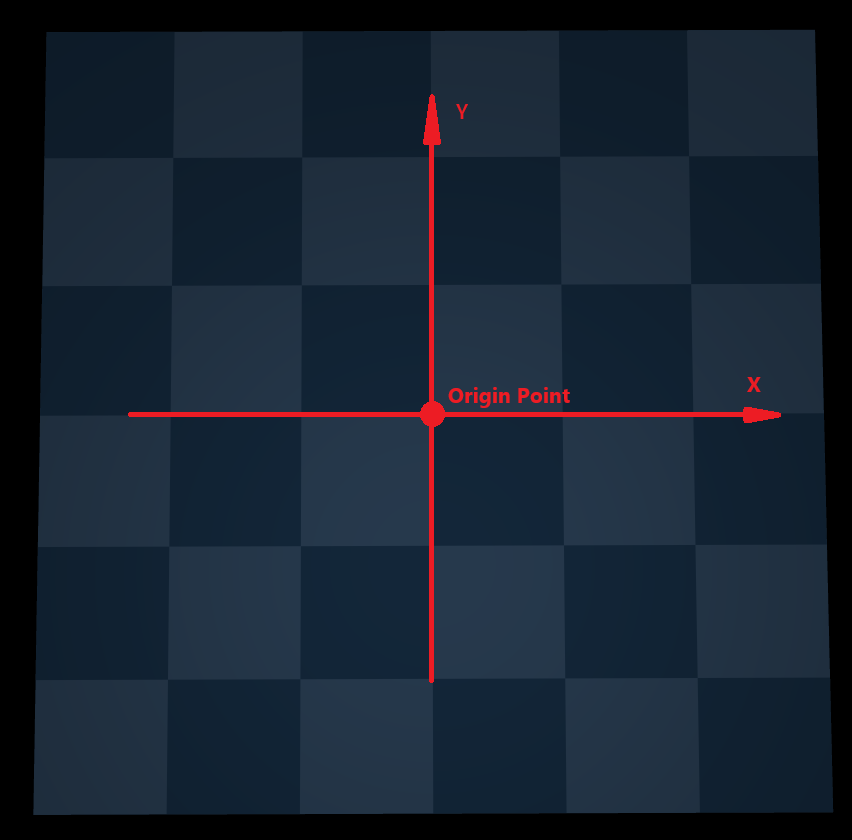
\includegraphics[width=0.5\linewidth]{floor.jpg}
\caption{\label{fig:floor}The Floor of The Simulation Environment.}
\end{figure}


\subsubsection{Simulation environment}
To block the robot from moving out of the floor, four walls were placed at (3, 0, 0) m, (-3, 0, 0) m, (0, 3, 0) m, and (0, -3, 0) m, with a thickness of 0.1 m. 

Because the robot's task is a pick-and-place task, we add two tables as picking places at (1.0, -2.5, 0.27) m and (-1.0, -2.5, 0.27) m. 
The tables are modeled as cuboids with dimensions 0.02 m × 0.01 m × 0.01 m (length × width × height). 
Placing places are added as two pairs of plates, one pair is at (2.8, 1.0) m, and the other pair is at (2.8, -1.0) m. 
Each pair has a lower plate (height = 0.23 m) and an upper plate (height = 0.43 m). 
The lower plates are constructed as cylinders with a diameter of 0.23 m and a height of 0.01 m, while the upper plates have a diameter of 0.15 m. 
The locations of the walls, picking tables, and placing plates are shown in Figure~\ref{fig:walls&tables&plates}.


\begin{figure}[h]
\centering
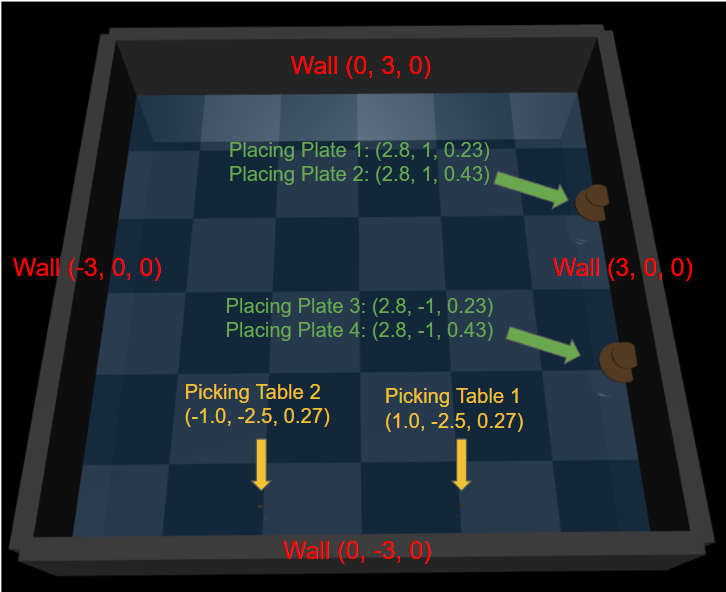
\includegraphics[width=0.7\linewidth]{walls&tables&plates.jpg}
\caption{\label{fig:walls&tables&plates} Locations of Walls, Picking Tables and Placing Plates.}
\end{figure}

The details of picking places and placing places are shown in the Figure~\ref{fig:tables&plates}.

\begin{figure}[h]
\centering
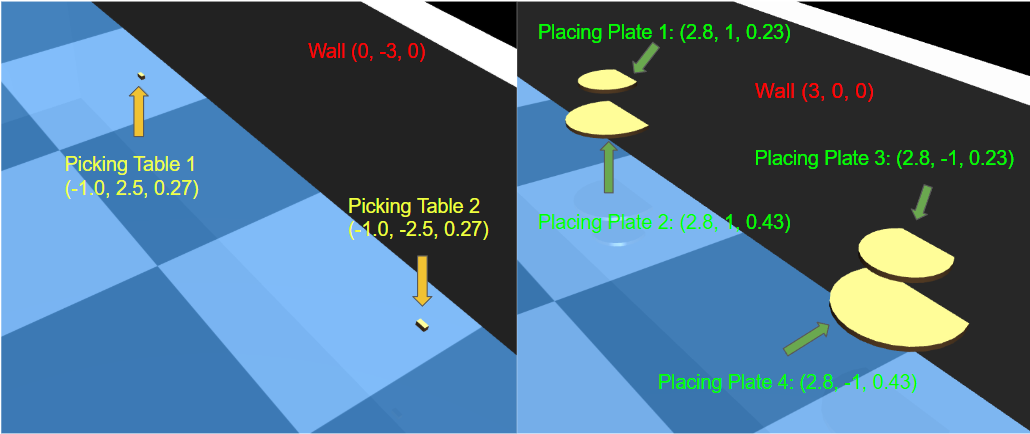
\includegraphics[width=0.7\linewidth]{tables&plates.jpg}
\caption{\label{fig:tables&plates}Details of Picking Tables and Placing Plates.}
\end{figure}

Ten objects are added for robots to perform the pick-and-place task. For locating objects on picking tables and removing objects from the placing plates, two threads were started --- a placer thread and a remover thread. The mechanism of the placer thread is to place an object on a random picking table and ensure that only one table is occupied by an object; it should be empty on another picking table. The function of the remover thread is to remove objects from four plates. Removal is executed after a delay or immediately according to a configuration. 

\begin{figure}[H]
\centering
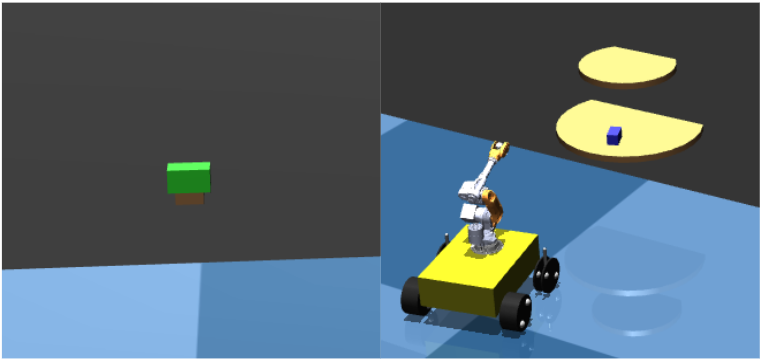
\includegraphics[width=0.7\linewidth]{object_on_a_table_and_plate.png}
\caption{\label{fig:object_on_a_table_and_plate}An Object on a Picking Table and an Object on a Placing Plate.}
\end{figure}

An AGV Robotic Arm is placed on (-1, 0) m as the primary robot. We will describe the modeling of the AGV Robotic Arm at the next section.

\subsubsection{Robot modeling}

This section presents the detailed modeling of the AGV Robotic Arm system implemented in the MuJoCo simulator. The system consists of a hybrid mobile manipulator designed for autonomous pick-and-place operations in warehouse environments. The robot combines wheeled mobility with a 5-DOF manipulator arm equipped with a vacuum-based end-effector for item manipulation.

The mobile platform employs an Ackermann steering geometry with four-wheel configuration. The chassis specifications were defined as follows:

\begin{table}[h]
\centering
\begin{tabular}{l|r}
Physical Parameters & Value \\\hline
Chassis dimensions (L×W×H) & 300mm × 220mm × 88mm \\
Total mass & 40 kg
\end{tabular}
\caption{\label{tab:widgets}Chassis Physical Parameters.}
\end{table}

The central point of Chassis was located at (-1, 0) m, which was the placement location of the AGV Robotic Arm mentioned in the preview section.

The drivetrain implemented a differential rear-wheel drive system with front-wheel steering:

\begin{table}[h]
\centering
\begin{tabular}{l|r|r}
Parameters & Left Wheel & Right Wheel \\\hline
Relative Position to Chassis Center & (-0.1, 0.12, -0.15) m &  (-0.1, -0.12, -0.15) m \\
\end{tabular}
\caption{\label{tab:widgets}Rear Wheel Specifications (Drive System).}
\end{table}

\begin{table}[H]
\centering
\begin{tabular}{l|r|r}
Parameters & Left Wheel & Right Wheel \\\hline
Relative Position to Chassis Center & 	(0.1, 0.15, -0.15) m &  (0.1, -0.15, -0.15) m \\
Steering Range & [-40°, +40°] (±0.698 rad) & [-40°, +40°] (±0.698 rad)  \\
\end{tabular}
\caption{\label{tab:widgets}Front Wheel Specifications (Steering System).}
\end{table}

In our MuJoCo simulation, two types of actuators are employed: a \textit{position actuator} for steering and a \textit{motor actuator} for driving. The steering actuator is attached to the front-wheel hinge and acts as a servo mechanism. Its control input $u \in [-0.9, 0.9]$ is scaled by a gear factor $g = 4.0$ to define a target angle $q_{\text{target}} = g \cdot u$. The applied torque follows a proportional-derivative control law,
\[
\tau = k_p \cdot (q_{\text{target}} - q) - k_d \cdot \dot{q},
\]
where $q$ and $\dot{q}$ denote the steering angle and angular velocity. In contrast, the driving actuator is a direct motor applied to the rear differential tendon. Its control input $u \in [-3, 3]$ is linearly mapped to torque through
\[
\tau = g \cdot u,
\]
with $g = 1.5$. The resulting torque is transmitted to the rear wheels via the tendon, producing forward or backward motion. In summary, the steering actuator regulates wheel orientation, while the driving actuator provides propulsion torque.


For each wheel, the radius is 0.05 m, and the mass is 0.125 kg.

The manipulator consists of a 5-DOF serial kinematic chain based on the WL-MiroPRO-6R200-05MM configuration:
\begin{table}[H]
\centering
\begin{tabular}{l|r|r|r}
Joint & Range (rad) & Mass (kg) & Link Geometry \\\hline
Joint 1 & [-3.142, 3.142] &  0.1 &  Base rotation \\
Joint 2 & [-0.611, 1.222] &  0.13 &  Shoulder \\
Joint 3 & [-1.565, 1.40] &  0.1 &  Elbow \\
Joint 4 & [-3.142, 3.142] &  0.045 &  Wrist pitch \\
Joint 5 & [-1.8, 2.2] &  0.015 &  Wrist roll \\
\end{tabular}
\caption{\label{tab:manipulator_joint_specs}Arm Joint Configuration.}
\end{table}


The vacuum adhesion was modeled using MuJoCo's adhesion actuator, The adhesion force $F_{adh}$ is computed as: $$F_{adh} = \min(u \cdot g \cdot A_{contact}, F_{max})$$

where:
\begin{itemize}
\item $u$ = control signal [0,1],
\item $g$ = gain parameter (4.0),
\item $A_{contact}$ = contact area,
\item $F_{max}$ = maximum adhesion force.
\end{itemize}

Following the official manual~\cite{wlkata_arm_doc}, the individual components of the manipulator were assembled within the simulation environment. The complete manipulator model was then mounted on the AGV described in the previous part, enabling subsequent evaluation of manipulation tasks in a mobile robotic setting.  

To provide a clear geometric representation of the manipulator, a three-view orthographic projection (front view, top view, and side view) is presented below. This visualization facilitates a better understanding of the overall structure and spatial configuration of the designed system in Figure~\ref{fig:robot_3_view}. The red arrows in the figure indicate the orientation direction of the robot. The AGV Robotic Arm system will be used for all the robots in case studies.

\begin{figure}[h]
\centering
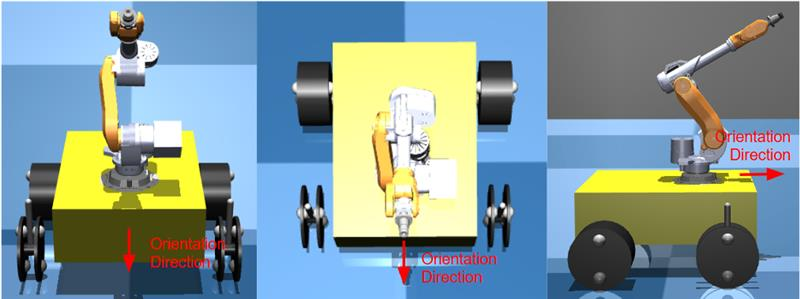
\includegraphics[width=0.7\linewidth]{robot_3_view.jpeg}
\caption{\label{fig:robot_3_view}Three-view Orthographic of the AGV Robotic Arm.}
\end{figure}

Next, we place an AGV Robotic Arm system as the primary robot in a simulation environment to provide readers with a clearer understanding of the experimental setup, as shown in Figure~\ref{fig:simenv_with_1st_robot}.

\begin{figure}[h]
\centering
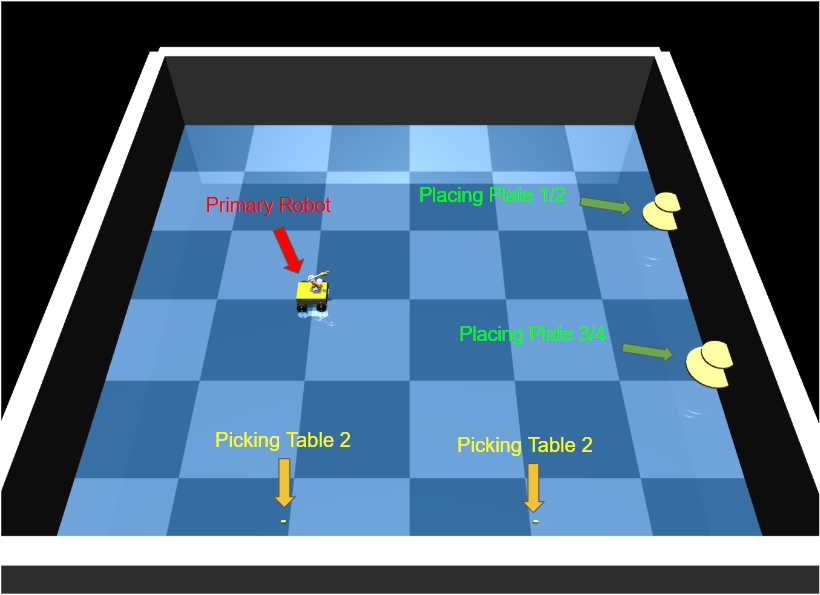
\includegraphics[width=0.6\linewidth]{simenv_with_1st_robot.png}
\caption{\label{fig:simenv_with_1st_robot}A Simulation Environment with a Primary Robot.}
\end{figure}

\subsubsection{Primary Robot Control for Pick-and-Place Task}

\paragraph{Overview} 
The primary robot is controlled using a scripted logic-based controller to perform pick-and-place operations in the simulated environment. 
The control system is responsible for executing sequences of pick and place motions.

\paragraph{Algorithm Description}
The control logic operates as follows:
\begin{enumerate}
    \item \textbf{Initialization:} Initialize all pickable objects in the environment. Initialize object placer/remover threads to manage the environment asynchronously.
    \item \textbf{Navigate to Pick Position and Pick Operation:} 
    \begin{itemize}
        \item From the origin position (-1, 0) m navigate the robot to the pick position, pick position is (1, -2.3) m if the next object is on picking table 1, (-1, -2.3) m if the next object is on picking table 2.
        \item Execute the pick motion to grasp the object.
    \end{itemize}
    \item \textbf{Navigate to Place Position and Place Operation:} 
    \begin{itemize}
        \item Navigate robot to pre-place position (0, 2) m.
        \item Select a placing plate pair randomly.
        \item Navigate to placing position, place position is (2.45, 1) m if the selected placing plate pair is placing plate 1 or 2, (2.51, -0.8) m if it is placing plate 3 or 4.
        \item Execute the placement motion to place the object onto the lower plate. 
        The remover thread will subsequently remove the placed object from the occupied plate 
        after a delay of 1000–2000 timesteps.
    \end{itemize}

\begin{figure}[H]
\centering
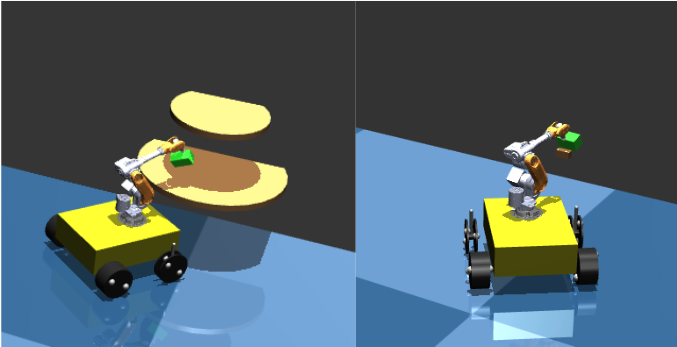
\includegraphics[width=0.5\linewidth]{pick_and_place.png}
\caption{\label{fig:pick_and_place}The Primary Robot is Placing and Picking.}
\end{figure}
    
    \item \textbf{Return to Origin Position:} 
    \begin{itemize}
        \item Navigate robot to pre-origin position (-2.5, 0) m.
        \item Navigate robot to origin position (-1, 0) m and reset all joints.
    \end{itemize}
    \item \textbf{Loop:} Repeat the pick-and-place sequence for all objects until the robot is in the origin position and no object is on the tables.
\end{enumerate}

\begin{algorithm}[H]
\caption{\label{alg:primary_robot_control_logic}Primary Robot Control Logic}
\KwIn{Initialized robot, objects, placer thread, and remover thread}
\KwOut{Completed pick-and-place cycles}

\While{task not completed}{
    Identify position of the object on the picking table\;
    Navigate to the pick position\;
    Execute pick motion\;
    Navigate to the pre-place position\;
    Rotate the arm to the front\;
    Select placing plate\;
    Navigate to the place position\;
    Execute place motion\;
    Navigate to the pre-origin position\;
    Return to origin and reset joints\;
}
\end{algorithm}


\begin{figure}[h]
\centering
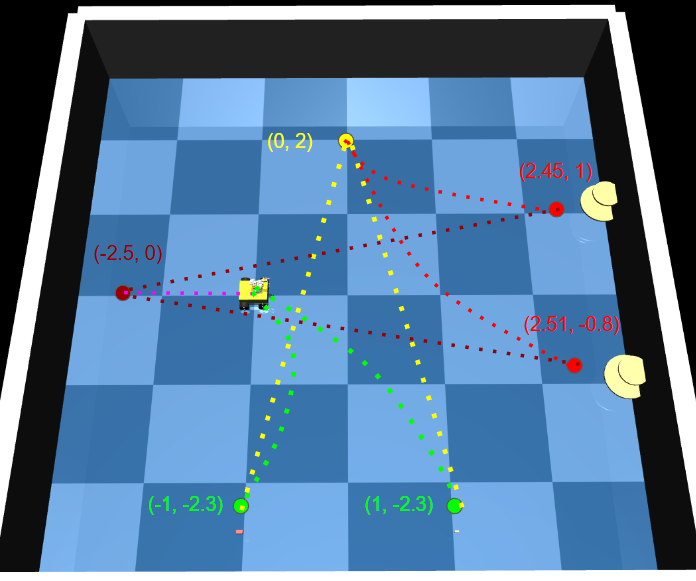
\includegraphics[width=0.5\linewidth]{primary_robot_working_path.png}
\caption{\label{fig:primary_robot_working_path}Working Path of the Primary Robot.}
\end{figure}

\subsection{Observation Algorithm for Pick-and-Place Task}

\paragraph{Motivation} 
To facilitate reinforcement learning training for a secondary agent, we design an observation algorithm that records the behavior of the primary robot during pick-and-place tasks. 
Specifically, it tracks the locations where the robot executes pick and place operations, which are used as task-relevant observations for the RL model.

\paragraph{Algorithm Description} 
The observation algorithm operates as follows:
\begin{enumerate}
    \item \textbf{Pick Detection:} Monitor the robot's end-effector to identify when a pick action is executed. The 3D coordinates of the object's position and the robot's position are recorded.
    \item \textbf{Place Detection:} Similarly, track the robot's end-effector for place actions, recording the coordinates of the placement fixture and the coordinates of the robot.
    \item \textbf{Observation Vector Construction:} Combine the recorded pick and place positions into a structured observation vector that serves as input for the reinforcement learning training.
\end{enumerate}

\begin{algorithm}[H]
\caption{Observation Algorithm for Pick-and-Place Tasks}
\KwIn{Number of loops $L$}
\KwOut{Object set $\mathcal{O}$, Placement set $\mathcal{P}$}

Initialize $\mathcal{O} \gets \emptyset$, $\mathcal{P} \gets \emptyset$\;

\For{$\ell \gets 1$ \KwTo $L$}{
    \tcp{Stage 1: Approach to Pick Position}
    Wait until the robot is near an object\;
    Identify the target object $o$\;
    Record object position $p_o$, size $s_o$, shape $f_o$, and robot position $r$\;
    Add $(p_o, s_o, f_o, r)$ to $\mathcal{O}$\;

    \tcp{Stage 2: Object Coupling}
    Detect robot-object coupling event (pick action complete)\;

    \tcp{Stage 3: Transport to Place Position}
    Track object in coupled state while the robot moves\;

    \tcp{Stage 4: Decoupling and Placement}
    Detect decoupling event (release)\;
    Identify the environment element $e$ (placement fixture) that contacts the object\;
    Record placement fixture position $q_o$, size $s_o$, shape $f_o$, and robot position $r$\;
    Add $(q_o, s_o, f_o, r)$ to $\mathcal{P}$\;
}
\Return{$\mathcal{O}, \mathcal{P}$}
\end{algorithm}

\paragraph{Purpose of Recording Observations}
During the pick-and-place task, we record key information about both the objects and the robot’s three-dimensional position at critical stages. 
The purpose of this observation process is to provide auxiliary information for subsequent reinforcement learning training. 
Specifically, these recorded observations serve three main roles: 
first, during the training of navigation models, they help define thresholds for determining whether the robot has reached target locations; 
second, in the training of pick and place models, they help initialize or constrain the robot’s starting configuration; 
third, in the training of high-level decision models, they restrict the legality of actions, ensuring that low-level policies are only executed when the robot is sufficiently close to the target object or placement location. 
Detailed usage of these observations is described in later sections.






\subsection{Reinforcement Learning Model Training}

After configuring the simulation environment, we introduce a secondary robot that is entirely controlled by the reinforcement learning (RL) model. The training framework is organized in a hierarchical manner, consisting of two layers: a low-level motor control layer and a high-level decision-making layer. This hierarchical design allows the secondary robot to perform pick-and-place tasks collaboratively with the primary robot while reducing the risk of conflicts. 

\paragraph{Low-Level Motor Control Layer}
The motor control layer is responsible for generating primitive actions of the secondary robot. It includes three categories of models:
\begin{itemize}
    \item \textbf{Navigation Models:} Two separate models are trained to control forward and backward movements of the robot base, enabling precise navigation in the simulation environment.
    \item \textbf{Pick Model:} A model dedicated to controlling the robotic arm to execute pick operations.
    \item \textbf{Place Model:} A model designed to control the robotic arm to perform place operations on an upper plate.
\end{itemize}

\paragraph{High-Level Decision-Making Layer}
The decision-making layer governs the overall task execution strategy of the secondary robot. This layer operates on a discrete action space, selecting which low-level control model should be triggered at each step. By learning an optimal policy, the decision-making layer coordinates navigation, picking, and placing actions in a context-aware manner. This enables the secondary robot to collaborate effectively with the primary robot in pick-and-place tasks while minimizing collisions between robots within the shared environment.

\subsubsection{Navigation Models Training}

\paragraph{Navigation Environment Formalism}

The navigation task for the secondary robot is formulated as a Markov Decision Process (MDP).

\subparagraph{State Space $\mathcal{S}$}
The state space integrates the instantaneous status of the secondary robot, the relative information of the primary robot and task, and multi-scale historical dynamics. Each component is normalized. The observation vector is defined as:
\[
\mathbf{o}_t = \big[ \mathbf{p}_2, \mathbf{v}_2, \theta_2, \; (\mathbf{p}_{g} - \mathbf{p}_2), d_{g}, \; \mathbf{r}_1, \mathbf{v}_1, \theta_1, \mathbf{v}_{1|2}, v^{rad}_{1|2}, \; \mathbf{s}_{task}, \; \mathbf{c}_{place}, \; \mathbf{h}_t \big],
\]
where
\begin{itemize}
    \item $\mathbf{p}_2 \in \mathbb{R}^2$, $\mathbf{v}_2 \in \mathbb{R}^2$, $\theta_2 \in [-\pi,\pi]$: position, velocity, and orientation (yaw) of the secondary robot,
    \item $\mathbf{p}_{g} \in \mathbb{R}^2$, $d_g \in \mathbb{R}$: relative position and distance to the target,
    \item $\mathbf{r}_1 \in \mathbb{R}^2$, $\mathbf{v}_1 \in \mathbb{R}^2$, $\theta_1 \in [-\pi,\pi]$: relative position, velocity, and orientation of the primary robot,
    \item $\mathbf{v}_{1|2} \in \mathbb{R}^2$, $v^{rad}_{1|2} \in \mathbb{R}$: velocity of Robot~1 relative to Robot~2, and corresponding radial velocity,
    \item $\mathbf{s}_{task} \in \{0,1\}^3$: task status flags, including FSM state index, whether Robot~2 is picking, and whether Robot~1 is carrying,
    \item $\mathbf{c}_{place} \in \{-1,0,1\}^4$: availability of the four placing plates, with values indicating overfilled, empty, or available,
    \item $\mathbf{h}_t \in \mathbb{R}^{36}$: multi-scale history features. For horizons $k \in \{5,10,20,50,100,200\}$, we extract
    \[
    \mathbf{h}_{t,k} = \big[ \mathbf{p}_1^{t-k}, \mathbf{p}_2^{t-k}, \Delta d_{1,2}^{t,k}, \tfrac{k}{200} \big],
    \]
    where $\mathbf{p}_1^{t-k}, \mathbf{p}_2^{t-k} \in \mathbb{R}^2$ are past positions of both robots, $\Delta d_{1,2}^{t,k}$ is the change in inter-robot distance since timestep $t-k$, and $\tfrac{k}{200}$ is a normalized time-scale weight.
\end{itemize}

The resulting observation vector is $61$-dimensional:
\[
\mathbf{o}_t \in \mathbb{R}^{61}.
\]



\subparagraph{Action Space $\mathcal{A}$}
The robot's navigation is controlled by the drive and steering systems. Therefore, the action space is
\[
\mathbf{a}_t = [a_{\min}, a_{\max}]^{2},
\]
where the first dimension corresponds to the drive system with range $[-3, 3]$ and the second dimension corresponds to the steering system with range $[-0.9, 0.9]$, the action space was applied normalization.

\subparagraph{Transition Dynamics $P$}
State transitions are governed by the MuJoCo simulator.

\subparagraph{Reward Function $R$}
The reward at each time step encourages progress toward the goal while penalizing inefficiency and unsafe behaviors:
\[
r_t = \underbrace{\alpha \cdot (d_{t-1} - d_t)}_{\text{progress reward}} + 
      \underbrace{\beta \cdot \mathbb{I}[d_t < \epsilon]}_{\text{arrival bonus}} +
      \underbrace{\lambda}_{\text{time penalty}} - 
      \underbrace{C_{forbidden} \cdot \mathbb{I}[\text{forbidden collision}]}_{\text{forbidden area penalty}},
\]
where
\begin{itemize}
    \item $d_t = \|\mathbf{p}_2 - \mathbf{p}_{goal}\|$ is the Euclidean distance from the secondary robot to the goal position of the current episode,
    \item $\alpha = 2000$ scales the reward for reducing the distance toward the goal,
    \item $\beta = 2000$ is the terminal bonus when reaching the goal,
    \item $\lambda = -0.3$ penalizes each time step to encourage efficiency,
    \item $C_{forbidden} = 2000$ penalizes collisions with forbidden zones.
\end{itemize}

\subparagraph{Termination Conditions}
An episode terminates under one of the following conditions:
\begin{enumerate}
    \item $d_t < \epsilon$ (goal reached),
    \item collision with forbidden regions,
    \item exceeding maximum time steps $T_{max} = 5000$,
    \item numerical instability in MuJoCo dynamics (e.g., $\text{qacc}$ divergence).
\end{enumerate}

\subparagraph{Goal Threshold $\epsilon$}
To determine whether the robot has reached the target, the threshold is defined as the minimal Euclidean distance between the robot's $(x, y)$ position $r$ and the $(x, y)$ coordinates of either objects $p_o$ or placement fixtures $q_o$ recorded in the observation algorithm (sets $\mathcal{O}$ and $\mathcal{P}$). This criterion ensures sufficient accuracy for reinforcement learning tasks. In our setup, we set $\epsilon = 0.2$. For example, when an object is located at $(-1.0, -2.5, 0.27)$ m and the robot's pick position is $(-1.0, -2.3)$ m, the Euclidean distance in the $(x, y)$ plane is $0.2$ m, which corresponds to the minimal value used to define the threshold.


\paragraph{Training Environment}

The training setups differ for the forward and backward navigation models:

\subparagraph{Forward Navigation Model}
The initial position of the secondary robot is set to $\mathbf{p}_{\text{2 init}} = (-2, 0)\,\text{m}$. 
For each episode, the goal position $\mathbf{p}_{\text{goal}}$ is randomly sampled from the set 
$\{(2, 2)\,\text{m}, (2, -2)\,\text{m}\}$.
The initial orientation of the secondary robot is aligned with the positive $x$-axis; the initial position of the secondary robot and goal positions are shown in Figure~\ref{fig:forward_model_training}.

\begin{figure}[H]
\centering
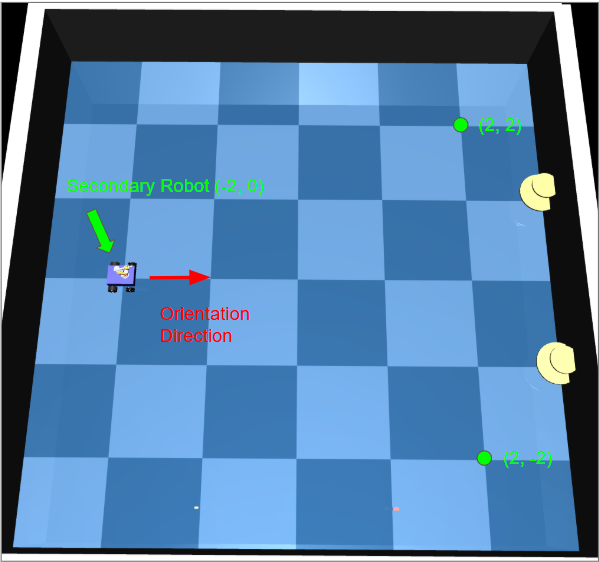
\includegraphics[width=0.6\linewidth]{forward_model_training.png}
\caption{\label{fig:forward_model_training}The Initial Position of Secondary Robot and Goal Positions for Forward Model Training.}
\end{figure}

\subparagraph{Backward Navigation Model}
The initial position of the secondary robot is set to $\mathbf{p}_\text{2 init} = (2, 0)$ m. For each episode, the $\mathbf{p}_{goal}$ is randomly sampled from the set $\{(-2, 2)\,\text{m}, (-2, -2)\,\text{m}\}$.
The initial orientation of the secondary robot is aligned with the positive $x$-axis; the initial position of the secondary robot and goal positions are shown in Figure~\ref{fig:backward_model_training}.

\begin{figure}[H]
\centering
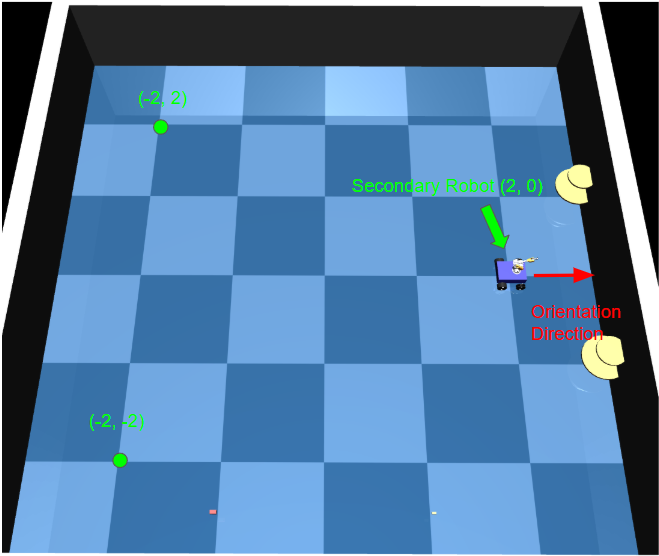
\includegraphics[width=0.6\linewidth]{backward_model_training.png}
\caption{\label{fig:backward_model_training}The Inital Position of Secondary Robot and Goal Positions for Backward Model Training.}
\end{figure}

\subparagraph{Training Configuration}

We employ $n=8$ parallel environments. The PPO models are trained with the following hyperparameters and configurations:
\begin{itemize}
    \item Learning rate: $1 \times 10^{-4}$
    \item Number of steps per environment per update: $n_{\text{steps}} = 1024$
    \item Batch size: $128$
    \item Number of epochs per update: $8$
    \item Entropy coefficient: $\alpha_{\text{ent}} = 0.02$ (exponentially decayed to $0.001$)
    \item Value function coefficient: $1.0$
    \item Clipping range: $0.15$
    \item Generalized Advantage Estimation parameter: $\lambda = 0.95$
    \item Total timestamps: $28 \times 10^6$
\end{itemize}


\paragraph{Training Results}

This section presents the performance evaluation of the forward and backward navigation models during training.

\subparagraph{Performance Metrics}
Training performance is evaluated based on the following metrics:
\begin{itemize}
\item \textbf{Average Episode Reward:} The mean reward obtained per training episode, indicating the overall quality of the learned policy.
\item \textbf{Success Rate:} The proportion of episodes in which the agent successfully reaches the goal position in a test set.
\end{itemize}

\subparagraph{Navigation Model Results}
The training results for the navigation models (forward and backward) are summarized as follows:
\begin{itemize}
\item Both models exhibited well-converged average episode reward curves (Figures~\ref{fig:avg_epi_rewerd_models}).
\item After $28 \times 10^{6}$ timesteps of training, each model achieved a final success rate of $\mathbf{100\%}$ on their respective test sets:
\begin{align*}
&\text{Forward model: } \{(2, 0)\,\text{m}, (2, 1)\,\text{m}, (2, -1)\,\text{m}, (1, 2)\,\text{m}, (1, -2)\,\text{m}\}, \quad \mathbf{p}_{\text{2 init}} = (-2, 0)\,\text{m}, \\
&\text{Backward model: } \{(-2, 0)\,\text{m}, (-2, 1)\,\text{m}, (-2, -1)\,\text{m}, (-1, 2)\,\text{m}, (-1, -2)\,\text{m}\}, \quad \mathbf{p}_{\text{2 init}} = (2, 0)\,\text{m}.  
\end{align*}
\item Both tests used identical parameters: $\epsilon = 0.2,\text{m}$, $20$ episodes per goal, and deterministic policy set to True.
\end{itemize}


\begin{figure}[h]
\centering
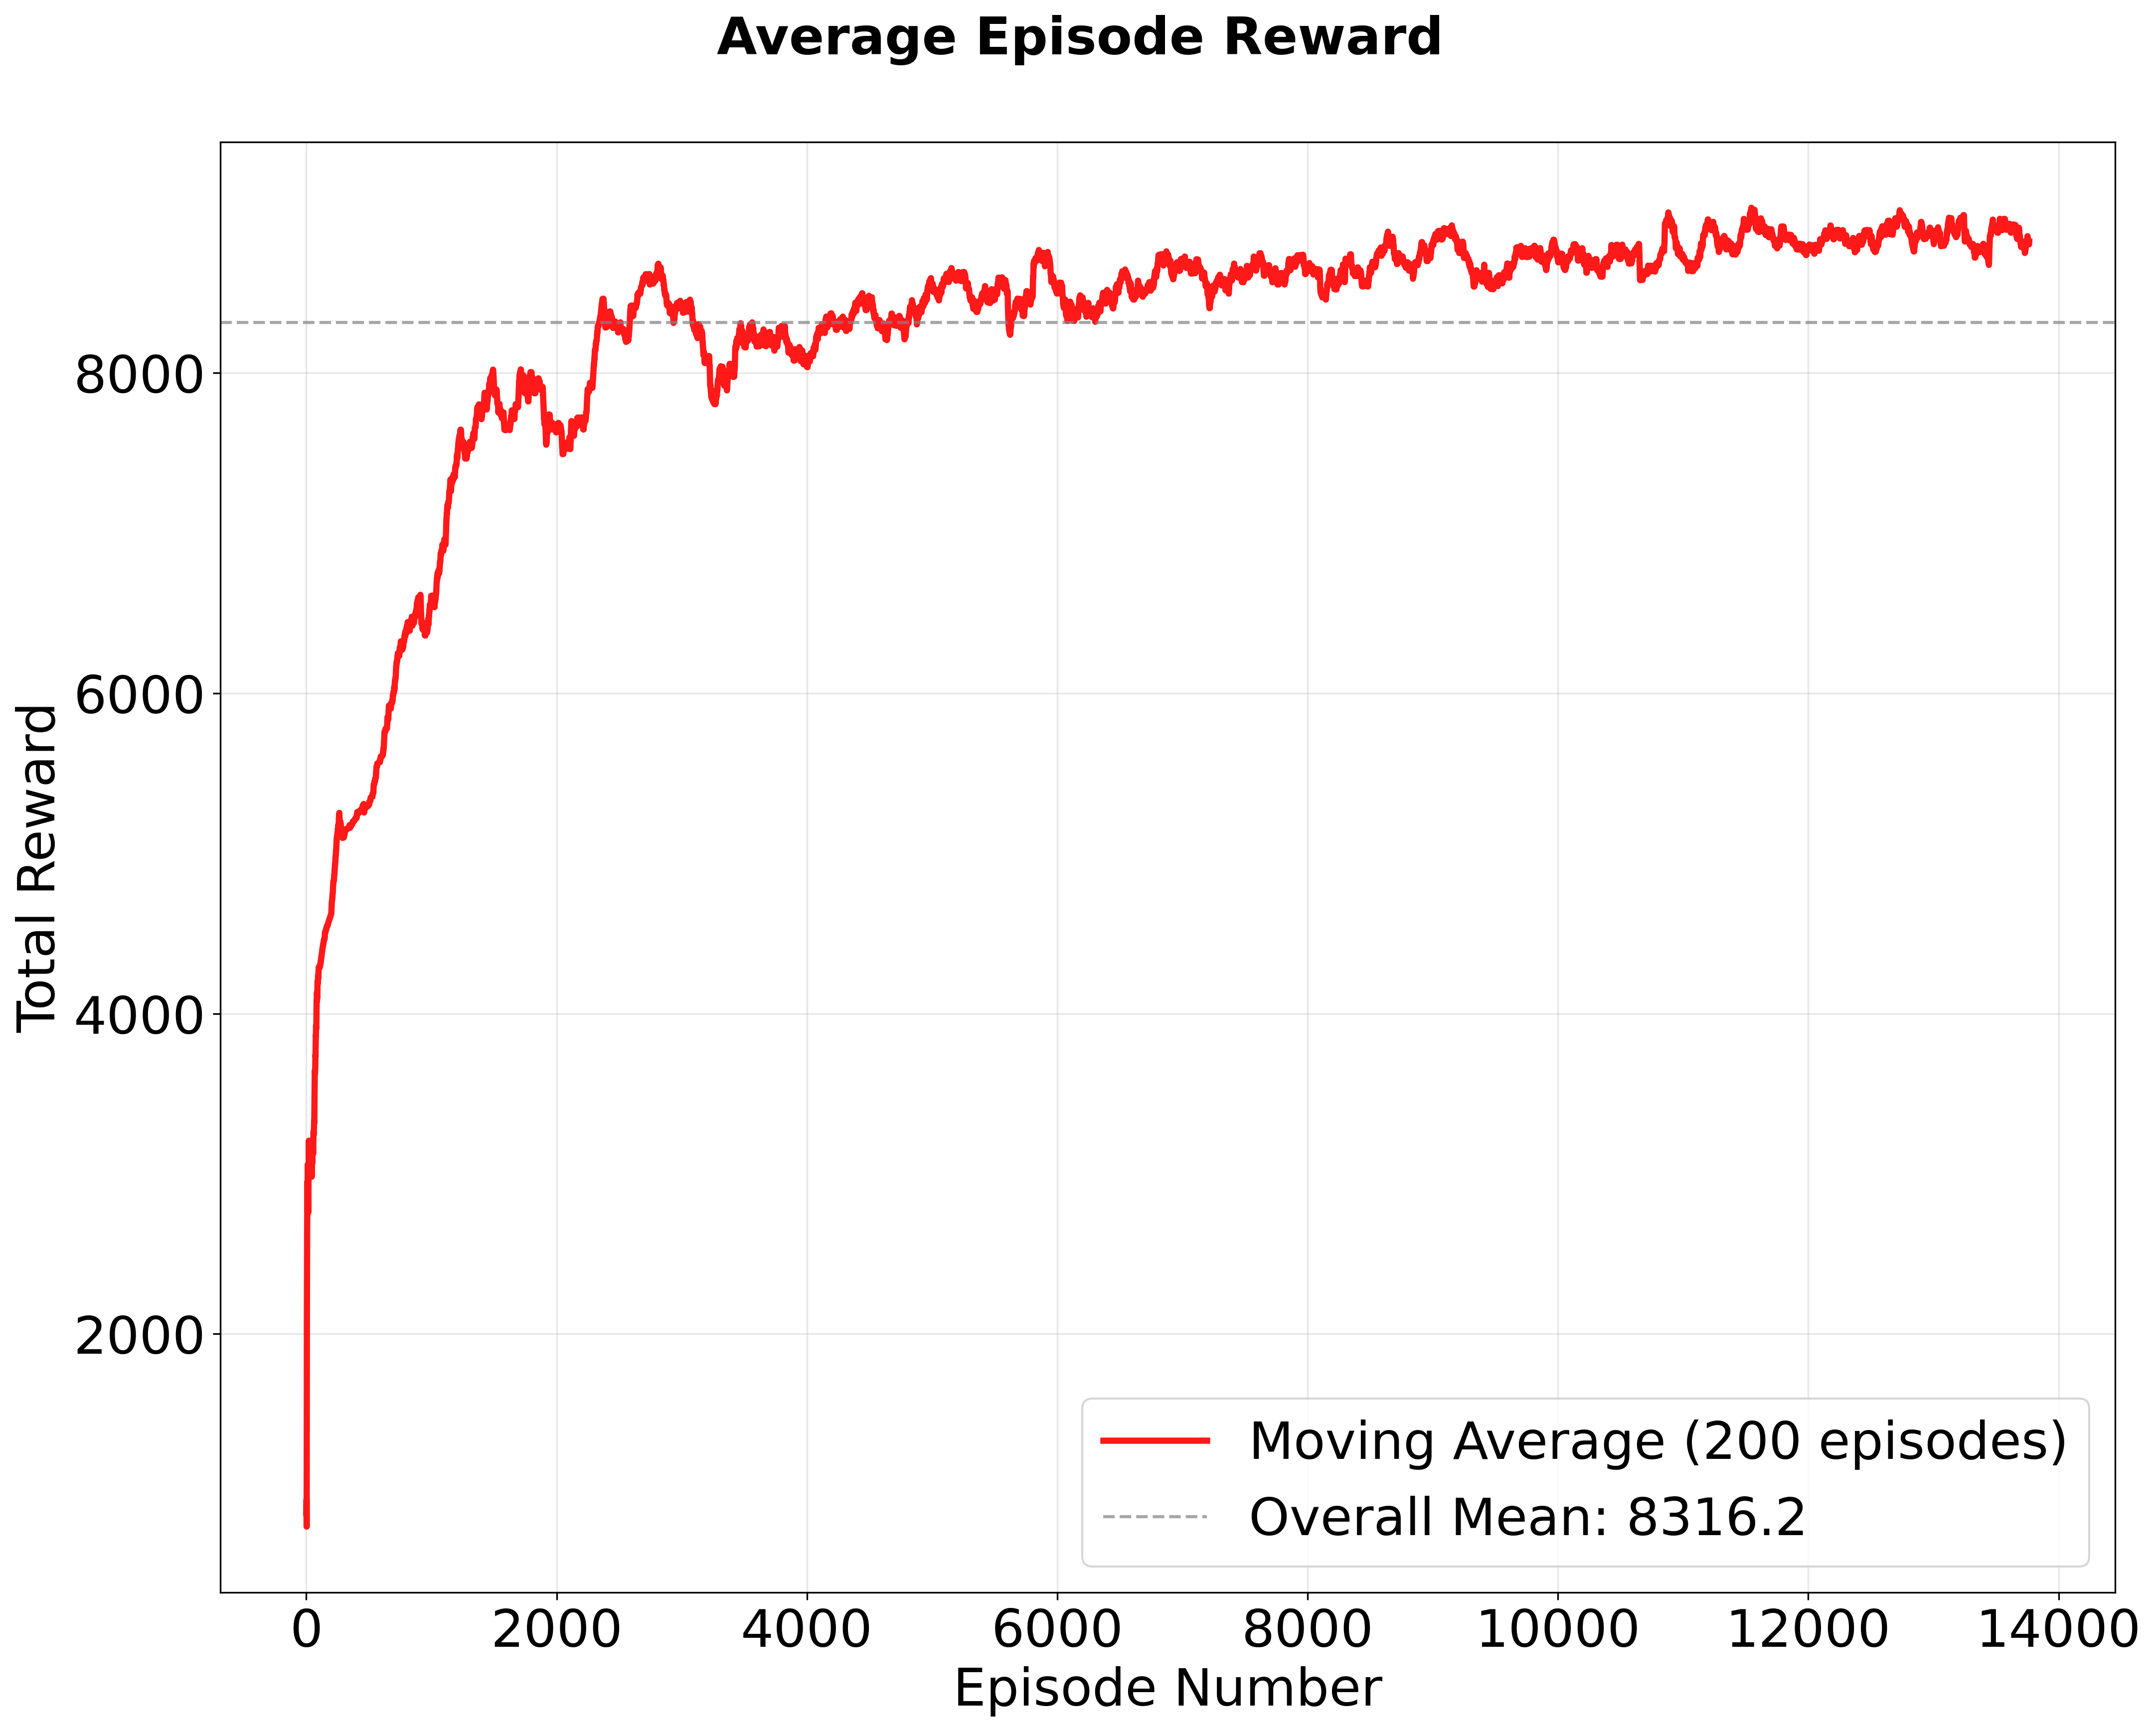
\includegraphics[width=0.45\linewidth]{avg_epi_rewerd_forward_model.png}
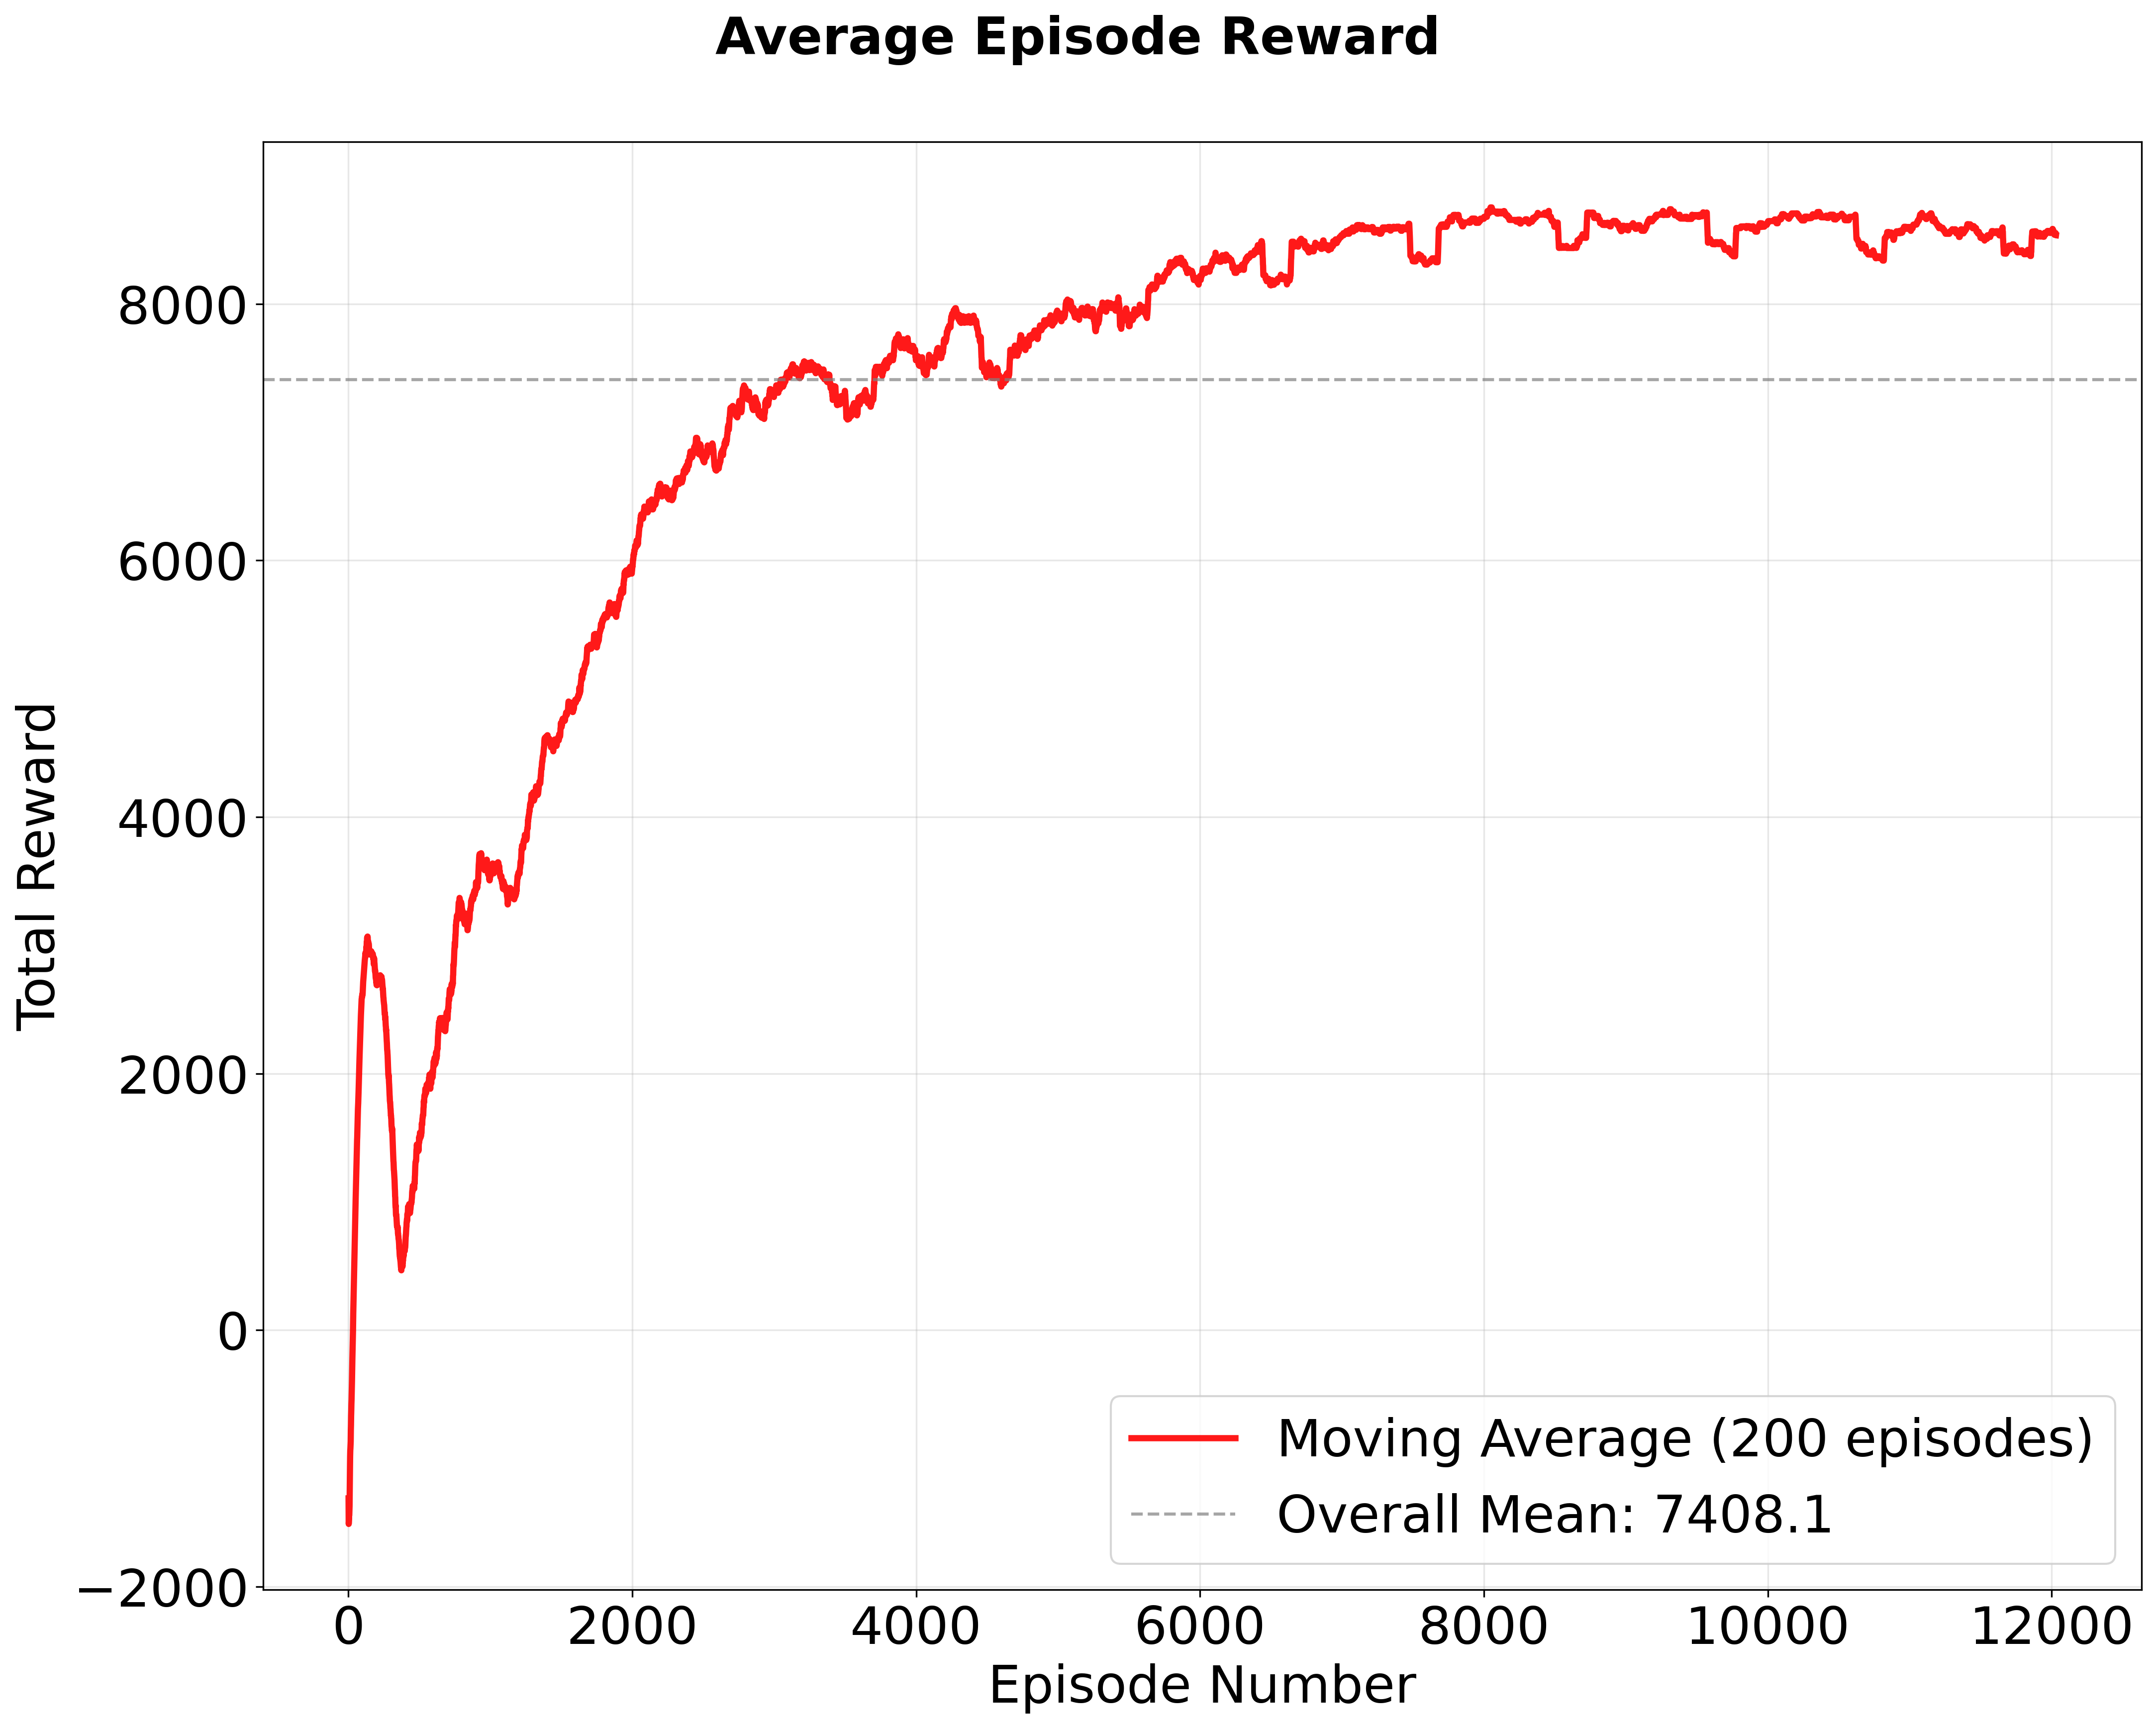
\includegraphics[width=0.45\linewidth]{avg_epi_rewerd_backward_model.png}
\caption{\label{fig:avg_epi_rewerd_models}Average Episode Reward Curves for the Forward (left) and Backward (right) Navigation Model Training.}
\end{figure}


\subsubsection{Pick Model Training}

\subparagraph{State Space $\mathcal{S}$}
The state space consists of the robot's proprioceptive state, end-effector information, target-relative features, and sensor readings, all components were normalized. The observation vector is constructed as:
\[
o_t = \big[ \mathbf{s}_{\text{self}}, \mathbf{s}_{\text{control}}, \mathbf{s}_{\text{sensor}}, \mathbf{s}_{\text{target}}, \mathbf{s}_{\text{orientation}} \big],
\]
where
\begin{itemize}
    \item $\mathbf{s}_{\text{self}} \in \mathbb{R}^8$ encodes the robot's self-state: position $\mathbf{p}_2 \in \mathbb{R}^3$, orientation $\theta_2 \in [-\pi,\pi]$, end-effector contact position $\mathbf{p}_{\text{contact}} \in \mathbb{R}^3$, and linear velocity $\mathbf{v}_{\text{ee}} \in \mathbb{R}^3$,
    \item $\mathbf{s}_{\text{control}} \in \mathbb{R}^6$ represents current control signals: vacuum adherence $a_{\text{vacuum}} \in [0,1]$ and joint controls $\mathbf{a}_{\text{joints}} \in [-1,1]^5$,
    \item $\mathbf{s}_{\text{sensor}} \in \mathbb{R}$ contains touch sensor activation $s_{\text{touch}} \in [0,1]$,
    \item $\mathbf{s}_{\text{target}} \in \mathbb{R}^6$ encodes target information: relative position $\mathbf{p}_{\text{rel}} \in \mathbb{R}^3$, distance $d_{\text{target}} \in \mathbb{R}^+$, horizontal angle $\theta_{xy} \in [-\pi,\pi]$, and vertical angle $\theta_z \in [-\pi,\pi]$,
    \item $\mathbf{s}_{\text{orientation}} \in \mathbb{R}^4$ represents end-effector orientation as a quaternion $\mathbf{q}_{\text{ee}} \in \mathbb{S}^3$.
\end{itemize}

\subparagraph{Action Space $\mathcal{A}$}
The action space consists of 6-dimensional continuous control signals mapped to specific joint ranges:
\[
\mathbf{a}_t = [a_1, a_2, a_3, a_4, a_5, a_{\text{vacuum}}] \in [-1,1]^6,
\]
where each dimension is mapped to actuator ranges according to Table~\ref{tab:manipulator_joint_specs} in the section of robot modeling:
\begin{itemize}
    \item Joint1: $a_1 \in [-1,1] \rightarrow [-3.142, 3.142]\,\text{rad}$
    \item Joint2: $a_2 \in [-1,1] \rightarrow [-0.611, 1.222]\,\text{rad}$
    \item Joint3: $a_3 \in [-1,1] \rightarrow [-1.565, 1.40]\,\text{rad}$
    \item Joint4: $a_4 \in [-1,1] \rightarrow [-3.142, 3.142]\,\text{rad}$
    \item Joint5: $a_5 \in [-1,1] \rightarrow [-1.8, 2.2]\,\text{rad}$
    \item Vacuum Suction: $a_{\text{vacuum}} \in [-1,1] \rightarrow [0,1]$
\end{itemize}

\subparagraph{Reward Function $R$}
The reward function encourages efficient picking behavior while penalizing unstable operations and collisions:
\[
\begin{aligned}
r_t = & \underbrace{1000 \cdot (d_{t-1} - d_t)}_{\text{distance reward}} + 
       \underbrace{200 \cdot \mathbb{I}[\text{touch contact}]}_{\text{contact bonus}} +
       \underbrace{200 \cdot \mathbb{I}[\text{suction activated}]}_{\text{picking bonus}} \\
      & + \underbrace{2000 \cdot \mathbb{I}[\text{picking\_stable\_steps} \geq 10]}_{\text{success bonus}}
     - \underbrace{0.1}_{\text{time penalty}} - 
       \underbrace{\mathbb{I}[v > 0.5] \cdot v}_{\text{speed penalty}} -
       \underbrace{20 \cdot \mathbb{I}[\text{object moved improperly}]}_{\text{handling penalty}} \\
      & - \underbrace{20 \cdot \mathbb{I}[\text{forbidden collision}]}_{\text{collision penalty}}
\end{aligned}
\]
where
\begin{itemize}
    \item $d_t$ is the Euclidean distance from the end-effector to the target object,
    \item $v$ is the vacuum sphere linear velocity magnitude,
    \item Distance reward is clipped at $-100$ to prevent excessive penalties.
\end{itemize}

\subparagraph{Termination Conditions}
An episode terminates under one of the following conditions:
\begin{enumerate}
    \item $\text{picking\_stable\_steps} \geq 10$ (successful picking),
    \item Object moved improperly, including object dropped and object hit away by robotic arm,
    \item Collision with forbidden areas (e.g., a pick table),
    \item Maximum time steps exceeded $T_{max} = 2000$.
    \item numerical instability in MuJoCo dynamics (e.g., $\text{qacc}$ divergence).
\end{enumerate}

\subparagraph{Picking Stability Counter}
The $\text{picking\_stable\_steps}$ counter increments when both of the following conditions are satisfied simultaneously and continuously:
\begin{itemize}
    \item \textbf{Touch Contact:} Physical contact detected between the end-effector tip and the target object
    \item \textbf{Suction Activated:} Vacuum adhesion actuator enabled ($a_{\text{vacuum}} = 1$)
\end{itemize}

\paragraph{Training Environment}
The robot was initialized at three randomly sampled positions, with random orientations assigned to the end-effector. Each robot–object pair was positioned such that the Euclidean distance in the $(x,y)$ plane between the robot base and the target object was approximately $0.2\,\text{m}$ (within $\pm 0.01\,\text{m}$), the distance is defined according to the Euclidean distance between the robot's $(x, y)$ position $r$ and the $(x, y)$ coordinates of objects $p_o$ recorded in the observation algorithm. This criterion ensures sufficient accuracy for reinforcement learning tasks. The specific configurations were as follows:
\begin{enumerate}
\item Robot at $(-0.89, -2.33)\,\text{m}$, object at $(-1.0, -2.5, 0.27)\,\text{m}$ (Picking Table 2), $(x,y)$ plane distance $\approx 0.202\,\text{m}$.
\item Robot at $(1.069, -2.31)\,\text{m}$, object at $(1.0, -2.5, 0.27)\,\text{m}$ (Picking Table 1), $(x,y)$ plane distance $\approx 0.202\,\text{m}$.
\item Robot at $(-1.09, -2.33)\,\text{m}$, object at $(-1.0, -2.5, 0.27)\,\text{m}$ (Picking Table 2), $(x,y)$ plane distance $\approx 0.192\,\text{m}$.
\end{enumerate}
The robot orientations and positions, as well as the object position, are illustrated in Figure~\ref{fig:pick_env_setup}, corresponding sequentially from left to right.

\begin{figure}[H]
\centering
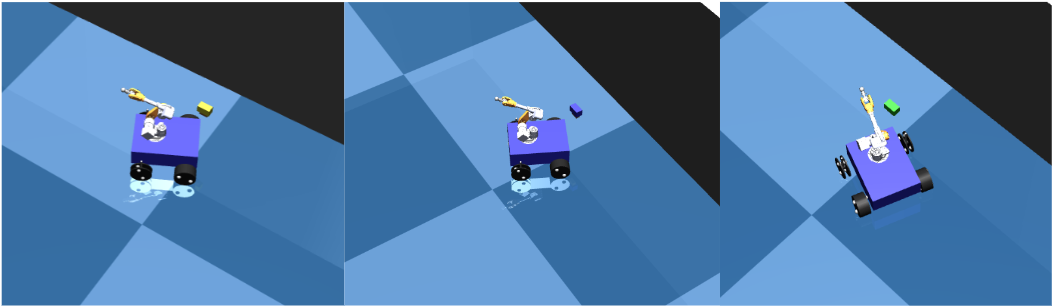
\includegraphics[width=1.0\linewidth]{pick_env_setup.png}
\caption{\label{fig:pick_env_setup}Initial robot–object configurations for the pick task environment. From left to right: the three sampled robot–object pairs described in the text.}
\end{figure}

For each of the three initial robot–object configurations described above, we trained an independent pick model to verify the formalism introduced in the previous sections. Each model was trained using the same reinforcement learning algorithm and hyperparameters to ensure consistency across experiments. This setup allows us to evaluate the robustness of the approach across different starting positions and orientations.

\subparagraph{Training Configuration}
Hyperparameters used for pick model training are shown as follows:
\begin{itemize}
    \item Environment number: 8
    \item Learning rate: $1 \times 10^{-4}$
    \item Number of steps per environment per update: $n_{\text{steps}} = 2048$
    \item Batch size: $256$
    \item Number of epochs per update: $8$
    \item Entropy coefficient: $\alpha_{\text{ent}} = 0.02$ (exponentially decayed to $0.0005$)
    \item Value function coefficient: $1.0$
    \item Clipping range: $0.15$
    \item Generalized Advantage Estimation parameter: $\lambda = 0.95$
    \item Total timestamps: $5 \times 10^6$
\end{itemize}

\paragraph{Training Results}

This section illustrates the training performance of the pick model. The performance is evaluated based on the average episode reward for each initial robot–object configuration. Figure~\ref{fig:pick_training_curves} presents the reward curves for the three trained pick models, displayed from left to right corresponding to the three initial configurations described in the previous section. All three models eventually converge to policies that successfully pick the target object.

\begin{figure}[H]
\centering
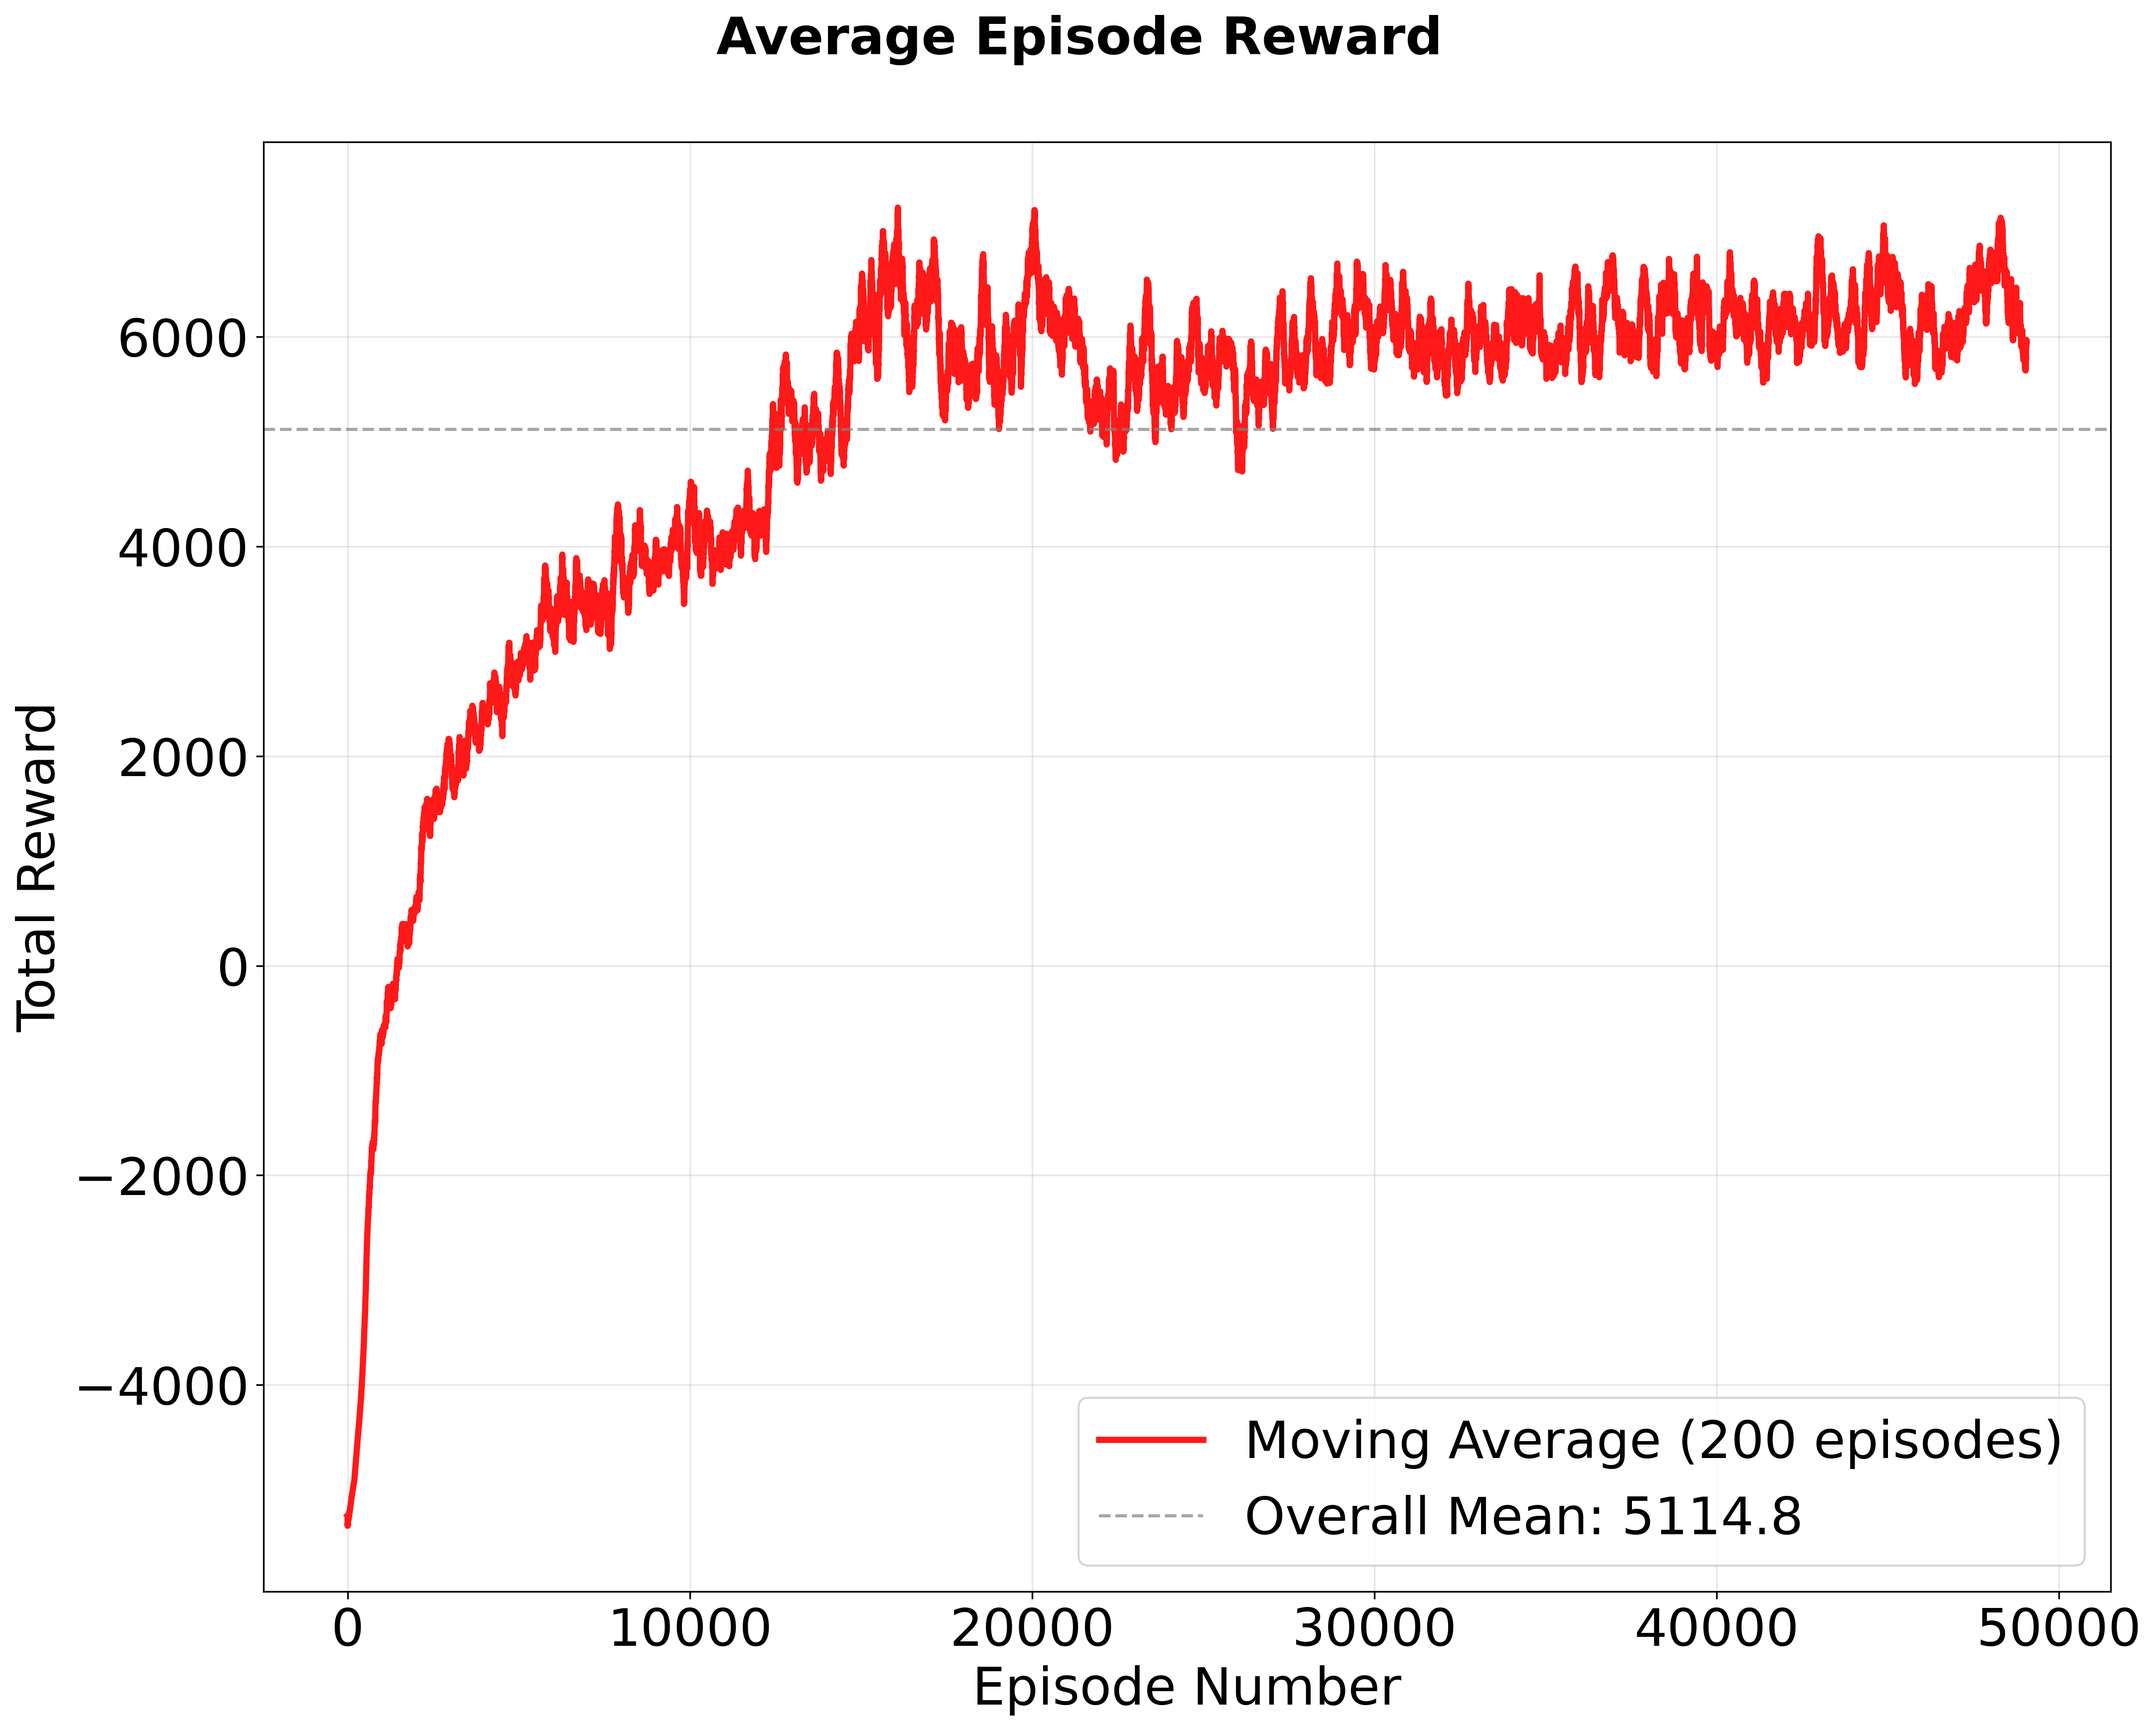
\includegraphics[width=0.32\linewidth]{pick_training_curves_1.png}
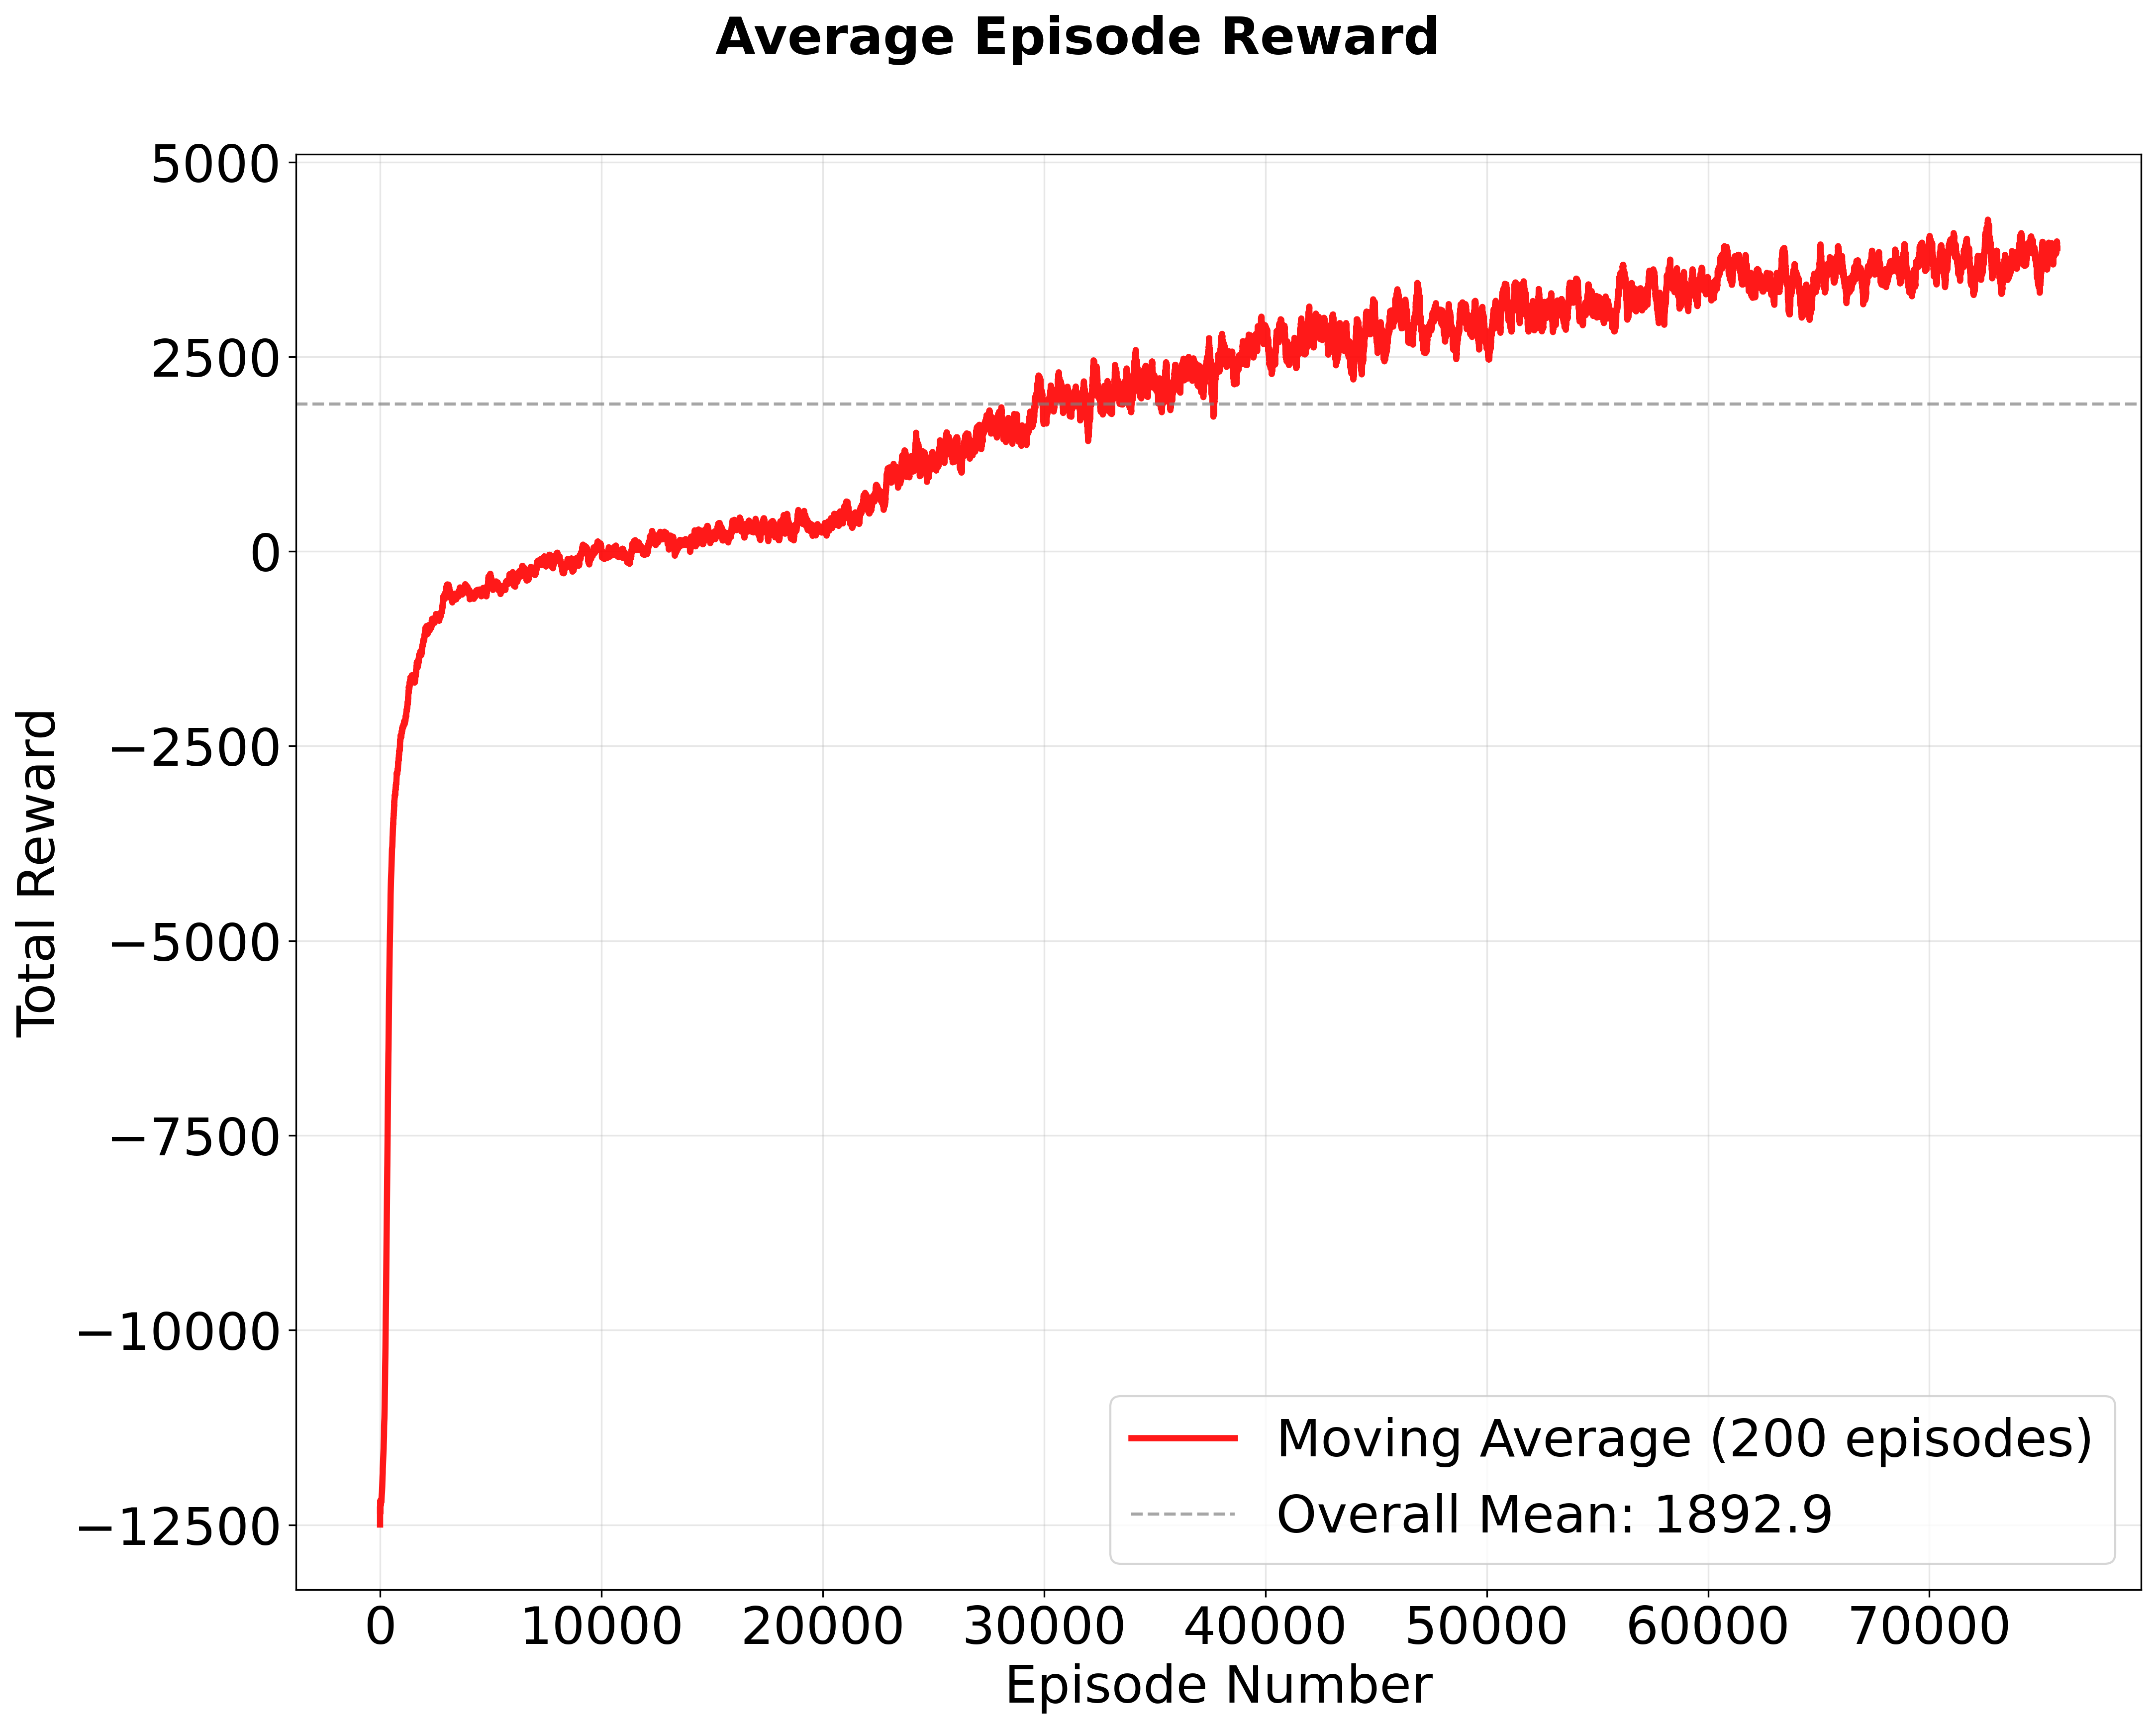
\includegraphics[width=0.32\linewidth]{pick_training_curves_2.png}
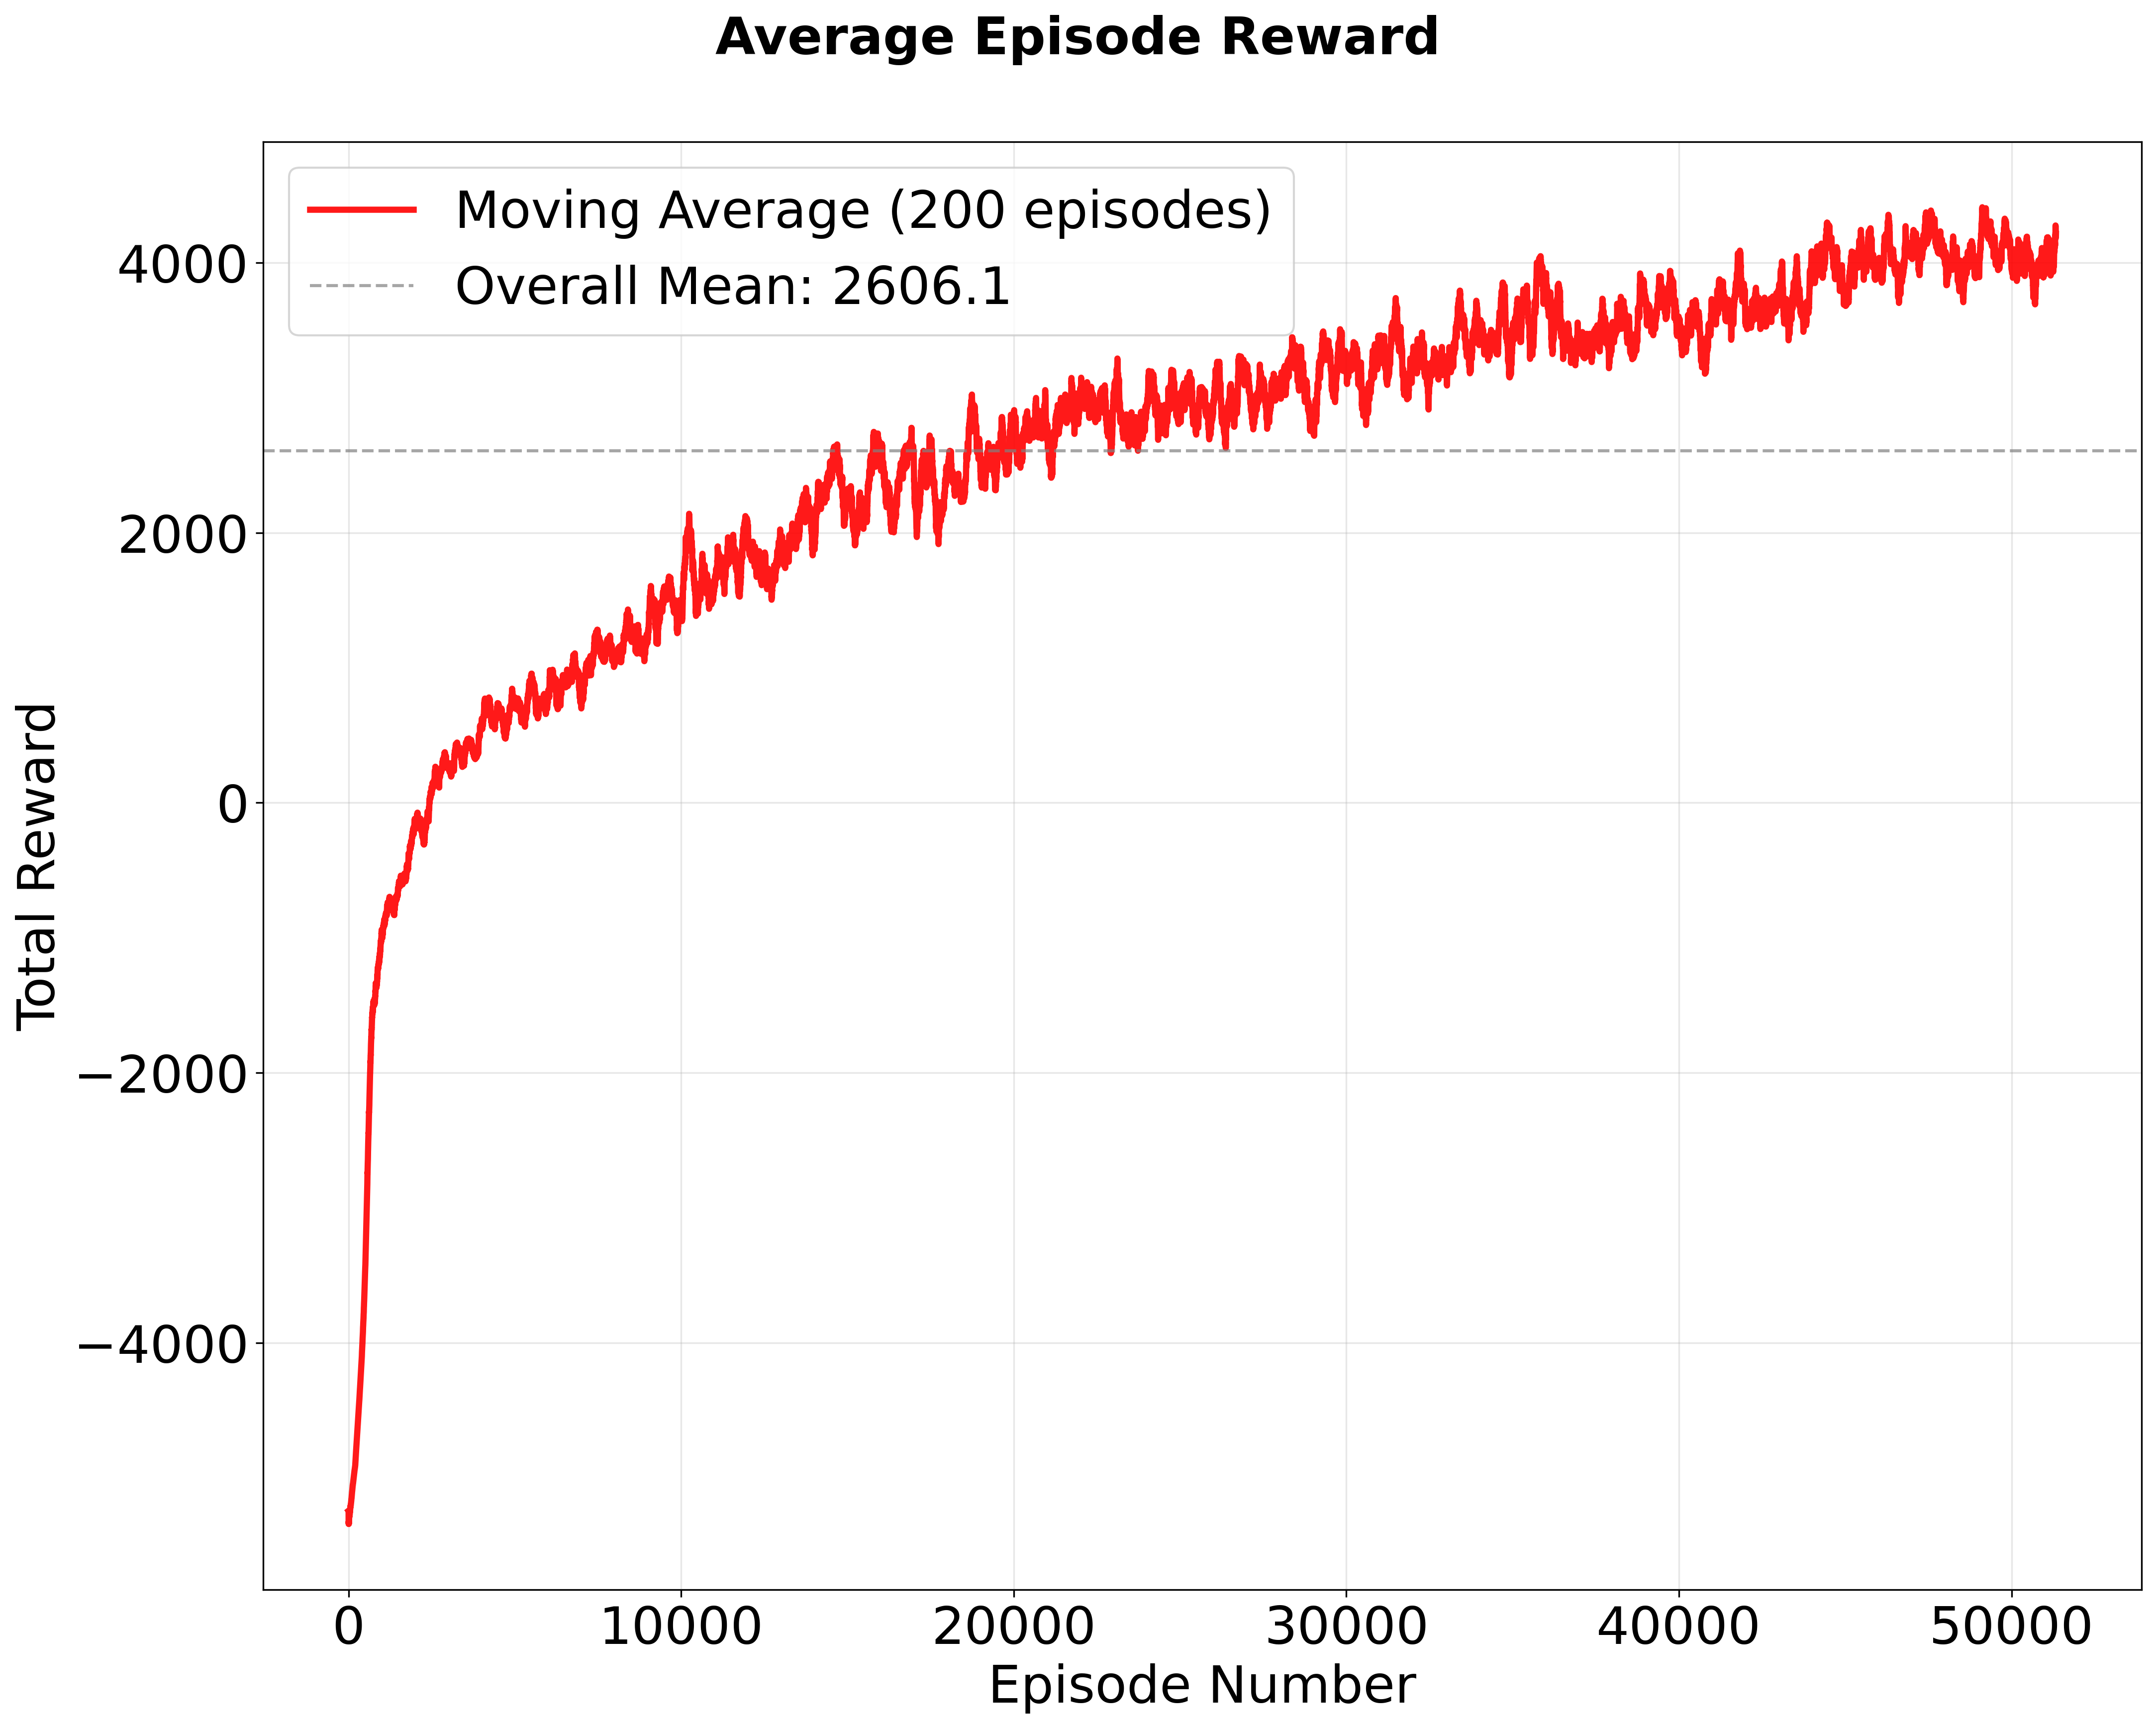
\includegraphics[width=0.32\linewidth]{pick_training_curves_3.png}
\caption{\label{fig:pick_training_curves}Average Episode Reward Curves for the pick model trainings.}
\end{figure}

While only three independent models were trained under specific configurations, without large-scale multi-domain training, the current results highlight the potential of the proposed formalism to yield generalized pick models once scaled to broader training domains.

\subsubsection{Place Model Training}
In our environment, a pair of placing plates consists of an upper and a lower layer. However, we restrict training to the case where the robot arm places objects on the upper plate. This is because the lower plate has a relatively larger surface area and is positioned below the lifting height of the robot arm, making successful placement there less challenging. In most cases, placing on the lower plate can be achieved simply by releasing the end-effector (setting the vacuum suction to zero). As illustrated in Figure~\ref {fig:placing_setup}, the focus of training is therefore on the upper plate scenario, which poses stricter requirements for precise control.

\begin{figure}[H]
\centering
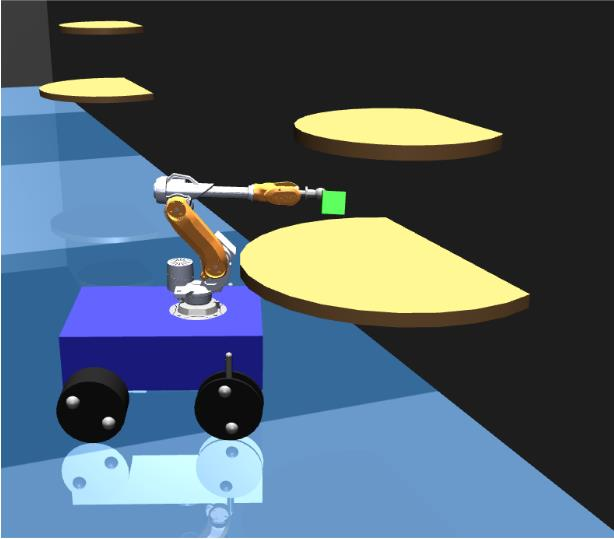
\includegraphics[width=0.32\linewidth]{placing_setup.jpeg}
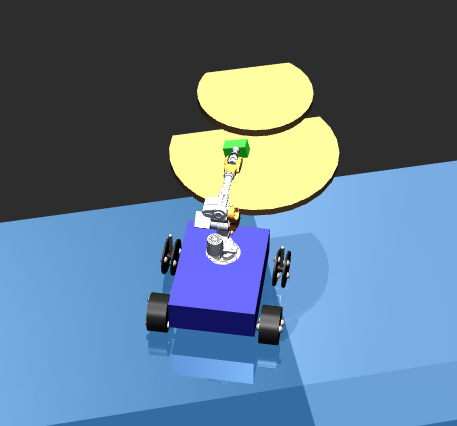
\includegraphics[width=0.301\linewidth]{placing_setup_2.png}
\caption{\label{fig:placing_setup}The secondary robot is preparing to place an object.}
\end{figure}

The goal is to move an object from its initial position to a target plate using a robot arm while avoiding collisions and dropping.

\subparagraph{State Space $\mathcal{S}$}
The state space includes object positions, velocities, actuator states, phase information, and safety indicators. The observation vector is constructed as:
\[
o_t = [o_\text{object}, o_\text{target}, o_\text{actuators}, o_\text{navigation}, o_\text{vacuum}, o_\text{phase}, o_\text{success}],
\]
where
\begin{itemize}
    \item $o_\text{object} \in \mathbb{R}^3$: normalized object position,
    \item $o_\text{target} \in \mathbb{R}^4$: target plane position and radius,
    \item $o_\text{actuators} \in \mathbb{R}^6$: normalized control signals of the 6 main actuators,
    \item $o_\text{navigation} \in \mathbb{R}^6$: relative position and angles from object to target,
    \item $o_\text{vacuum} \in \mathbb{R}^{16}$: vacuum sphere position, velocity, and orientation,
    \item $o_\text{phase} \in \mathbb{R}^{11}$: one-hot phase encoding, stage progress, horizontal/vertical distances, velocities, phase duration, safety indicators,
    \item $o_\text{success} \in \mathbb{R}$: indicator if the object is on the plane.
\end{itemize}

\subparagraph{Action Space $\mathcal{A}$}
The action space consists of a 5-dimensional continuous control signal for the robot actuators:
\[
\mathbf{a}_t = [a_1, a_2, a_3, a_4, a_5] \in [-1,1]^5,
\]
with each dimension mapped to actuator ranges as:
\begin{itemize}
    \item Joint1: $a_1 \in [-1,1] \rightarrow [-3.142, 3.142]\,\text{rad}$
    \item Joint2: $a_2 \in [-1,1] \rightarrow [-0.611, 1.222]\,\text{rad}$
    \item Joint3: $a_3 \in [-1,1] \rightarrow [-1.565, 1.40]\,\text{rad}$
    \item Joint4: $a_4 \in [-1,1] \rightarrow [-3.142, 3.142]\,\text{rad}$
    \item Joint5: $a_5 \in [-1,1] \rightarrow [-1.8, 2.2]\,\text{rad}$
\end{itemize}

\subparagraph{Reward Function $R$}
The reward function encourages efficient picking and stable placement while penalizing drops and collisions:

\[
\begin{aligned}
r_t = & \underbrace{r_\text{phase}}_{\text{phase progress reward (defined separately)}} +
       \underbrace{5.0 \cdot \mathbb{I}[\text{object on plate}]}_{\text{placement reward}} \\
      & - \underbrace{50 \cdot \mathbb{I}[\text{object dropped}]}_{\text{drop penalty}} -
       \underbrace{50 \cdot \mathbb{I}[\text{object detached from end-effector}]}_{\text{detachment penalty}} \\
      & - \underbrace{0.001}_{\text{time penalty (optional)}} 
\end{aligned}
\]

Here:

\begin{itemize}
    \item \textbf{Placement reward} is given for stable contact with the plate.
    \item \textbf{Drop penalty} is applied if the object falls.
    \item \textbf{Detachment penalty} is applied if the object detaches unexpectedly.
\end{itemize}

\subparagraph{Phase Mechanism}
The task is divided into four sequential phases:
\begin{itemize}
    \item \textbf{Horizontal Escape}: move object away from initial constrained region,
    \item \textbf{Vertical Lifting}: lift object to a safe height above the target plane,
    \item \textbf{Horizontal Approach}: approach target plane horizontally,
    \item \textbf{Precision Descent}: carefully lower object onto target plane.
\end{itemize}

\subparagraph{Phase-specific Rewards $r_\text{phase}$}
The reward $r_\text{phase}$ guides the agent through four sequential phases of object placement: \textit{horizontal escape}, \textit{vertical lifting}, \textit{horizontal approach}, and \textit{precision descent}. Each phase is determined by the object's position relative to the target plate and switches irreversibly once its completion criteria are satisfied. Denote the object position as $p_\text{obj} = (x, y, z)$, the target plate center as $p_\text{target}$, and the plate top height as $z_\text{plate}$.

\subparagraph{Phase Transitions}  
The current phase is selected according to the following criteria:
\begin{itemize}
    \item \textbf{Horizontal Escape $\to$ Vertical Lifting}: triggered once the horizontal escape distance $d_\text{escape} = \|p_\text{obj}^{xy} - p_\text{target}\| - r_\text{plate}$ exceeds $0.05$ m.
    \item \textbf{Vertical Lifting $\to$ Horizontal Approach}: triggered once the object height above the plate, $h_\text{lift} = z - z_\text{plate}$, exceeds $0.06$ m, after escape has completed.
    \item \textbf{Horizontal Approach $\to$ Precision Descent}: triggered once the horizontal distance to the plate center, $d_\text{approach} = \|p_\text{obj}^{xy} - p_\text{target}\|$, is less than $0.06$ m, after lifting has completed.
    \item \textbf{Precision Descent}: the final phase, active once both escape and lifting are complete and the approach condition is satisfied.
\end{itemize}
Phase switches are irreversible, and each transition grants a fixed bonus to encourage steady task progression.

\subparagraph{Reward Formulation}  
Within each phase, dense rewards measure progress toward the corresponding sub-goal, while small penalties prevent unsafe behaviors:

\begin{itemize}
    \item \textbf{Horizontal Escape (ESCAPE)}:
    \[
    r_\text{phase}^\text{ESCAPE} = 80 \cdot \Delta d_\text{rover} +
    \begin{cases}
        -0.05, & \text{if distance to plate bottom $< 0.03$ m} \\
        0, & \text{otherwise}
    \end{cases}
    \]
    where $\Delta d_\text{rover}$ is the change in horizontal distance to the rover. Positive progress (approaching the rover) is rewarded, negative progress is penalized. A small penalty discourages unsafe proximity to the plate bottom.

    \item \textbf{Vertical Lifting (LIFTING)}:
    \[
    r_\text{phase}^\text{LIFTING} = 80 \cdot \Delta h_\text{lift} +
    \begin{cases}
        -0.05, & \text{if horizontal distance to plate center $< 0.01$ m} \\
        0, & \text{otherwise}
    \end{cases}
    \]
    where $\Delta h_\text{lift}$ is the change in distance to a safe lifting height (6 cm). Upward progress is rewarded, downward deviation penalized.

    \item \textbf{Horizontal Approach (APPROACH)}:
    \[
    r_\text{phase}^\text{APPROACH} = 80 \cdot \Delta d_\text{approach} +
    \begin{cases}
        -0.05, & \text{if height above plate $< 0.03$ m} \\
        0, & \text{otherwise}
    \end{cases}
    \]
    where $\Delta d_\text{approach}$ is the reduction in horizontal distance to the plate center. Progress toward alignment is rewarded, divergence is penalized. Unsafe low heights incur a penalty.

    \item \textbf{Precision Descent (DESCENT)}:
    \[
    r_\text{phase}^\text{DESCENT} = 80 \cdot \Delta h_\text{descent} +
    \begin{cases}
        -0.05, & \text{if horizontal distance $> 0.08$ m} \\
        0, & \text{otherwise}
    \end{cases}
    \]
    where $\Delta h_\text{descent}$ is the reduction in vertical distance toward the target placement height (2 cm). Proper downward progress is rewarded, upward motion penalized. Misalignment beyond tolerance incurs a penalty.
\end{itemize}

\subparagraph{Termination Conditions}
An episode terminates under any of the following conditions:
\begin{enumerate}
    \item Object is successfully placed stably for the required number of steps (task success),
    \item Collision with forbidden areas or environment obstacles is detected,
    \item The object is dropped or detached from the end effector,
    \item Maximum steps of 32,000 are reached,
    \item Numerical instability detected in the simulation (e.g., $\text{qacc}$ values exceed threshold).
\end{enumerate}


Each phase is tracked with one-hot encoding in the state vector, and phase transitions grant bonus rewards to encourage smooth task progression.

\paragraph{Training Environment}
The robot was initialized at a random position with a random orientation. The reference distance to the center was approximately $0.35\text{m}$. This distance was determined based on the largest Euclidean distance between the robot’s $(x, y)$ position $r$ and the placement fixture’s $(x, y)$ coordinates $q_o$ as recorded by the observation algorithm. For example, the maximum Euclidean distance occurred when the robot was located at $(2.51, 0.8)\text{ m}$ and the placement fixture was positioned at $(2.8, -1)\text{ m}$ during the placement task performed by the primary robot. The specific position of the secondary robot is $(2.46, -0.90)\text{ m}$. The orientation and position of robot are shown in Figure~\ref{fig:placing_config}

\begin{figure}[H]
\centering
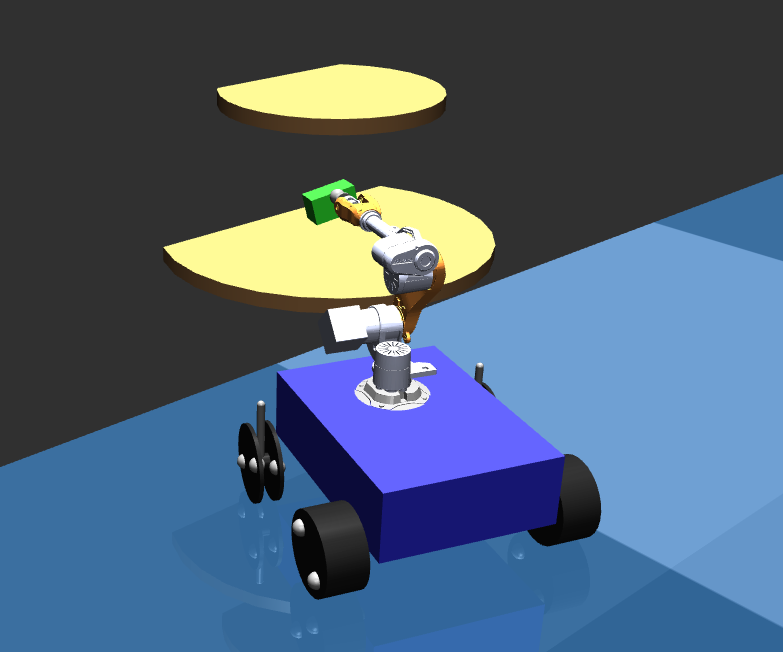
\includegraphics[width=0.5\linewidth]{placing_config.png}
\caption{\label{fig:placing_config}Initial position and orientation of The secondary robot for training.}
\end{figure}

\subparagraph{Training Configuration}
Hyperparameters used for place model training are shown as follows:
\begin{itemize}
    \item Environment number: 8
    \item Learning rate: $1 \times 10^{-4}$
    \item Number of steps per environment per update: $n_{\text{steps}} = 2048$
    \item Batch size: $256$
    \item Number of epochs per update: $10$
    \item Entropy coefficient: $\alpha_{\text{ent}} = 0.02$ 
    \item Value function coefficient: $1.0$
    \item Clipping range: $0.2$
    \item Generalized Advantage Estimation parameter: $\lambda = 0.95$
    \item Total timestamps: $4 \times 10^6$
\end{itemize}

\paragraph{Training Results}

This section reports the training outcomes of the pick model, assessed through the average episode reward under previous robot–object configuration. Figure~\ref{fig:place_training_curves} shows the reward trajectory of the model training. The model ultimately converge to effective policies capable of placing the object.

\begin{figure}[H]
\centering
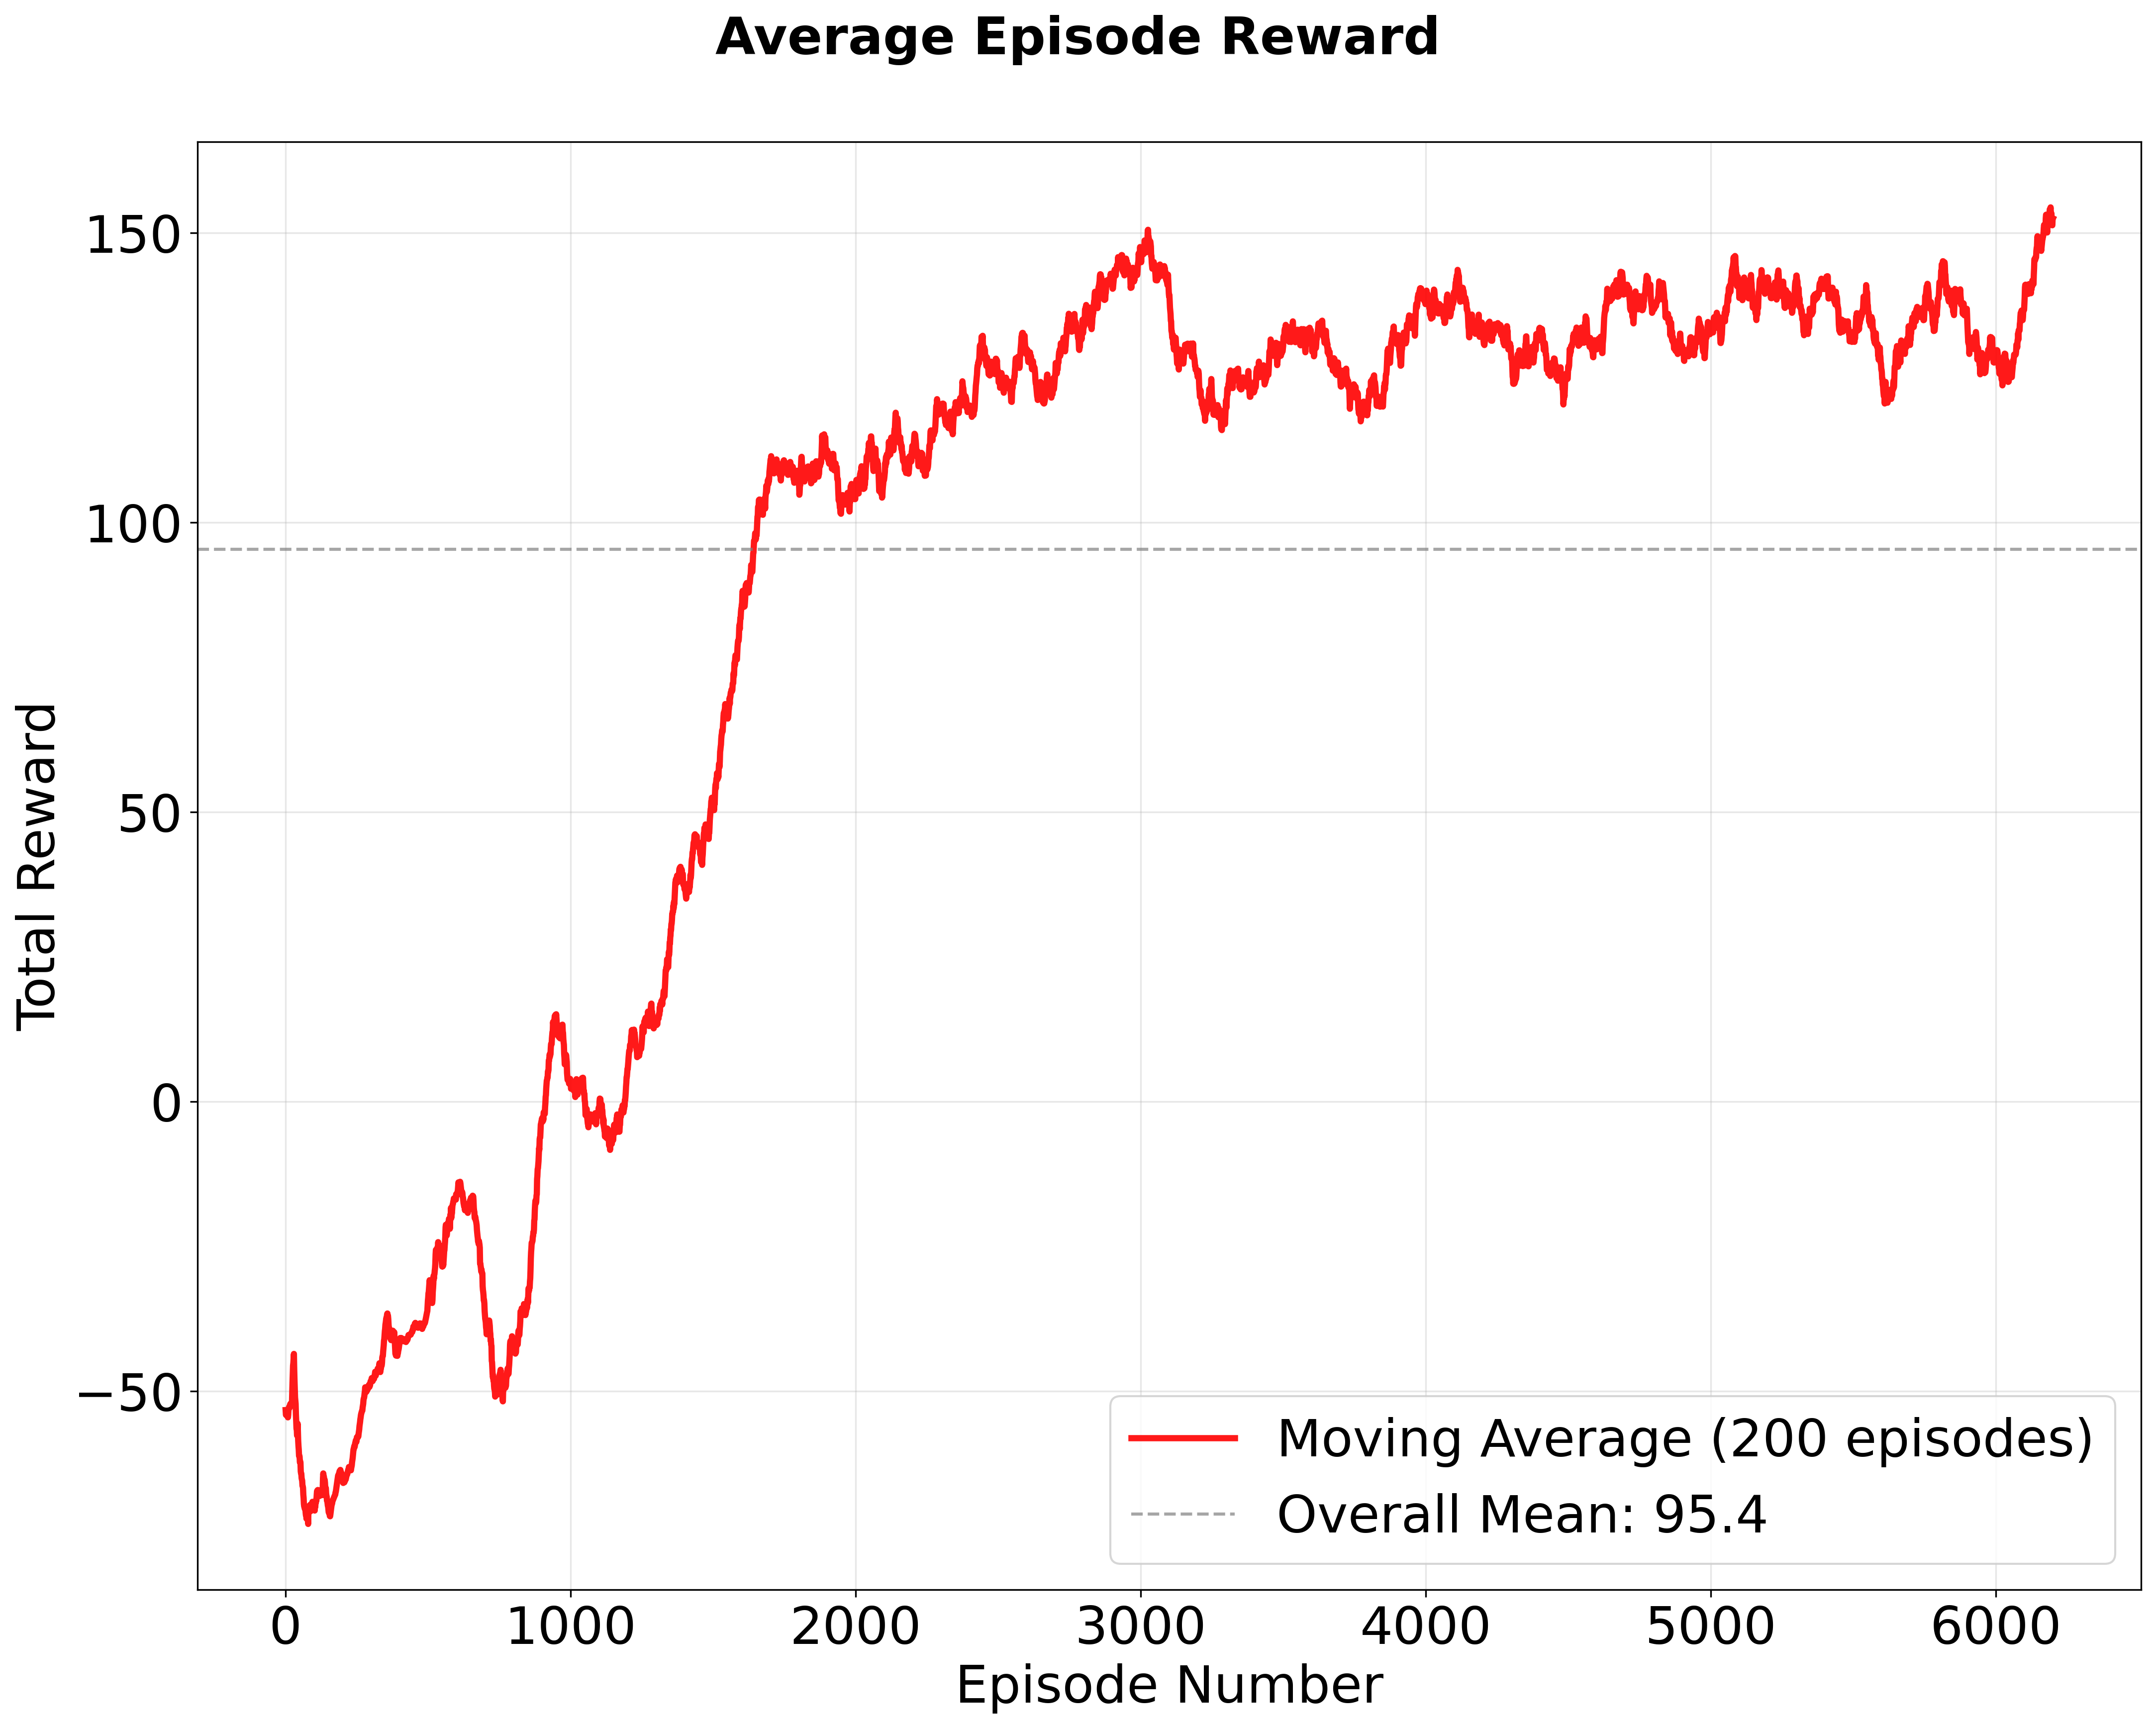
\includegraphics[width=0.7\linewidth]{place_training_curves.png}
\caption{\label{fig:place_training_curves}Average Episode Reward Curves for the the place model training.}
\end{figure}

It should be noted that the training was conducted under a single configuration rather than across diverse scenarios. Consequently, the resulting policy does not demonstrate generalization. Nonetheless, the outcome indicates that the proposed formalism can be extended to large-scale multi-domain training to obtain a generalized place model.

\subsubsection{Decision-making Model Training}

Building upon the previously trained submodules, we denote the forward navigation model as $\pi_{\text{nav}}^{f}$ and the backward navigation model as $\pi_{\text{nav}}^{b}$. In addition, we assume the availability of a generalized pick model $\pi_{\text{pick}}$ and a generalized place model $\pi_{\text{place}}$, as introduced in the preceding sections.

In this section, we focus on training a higher-level decision-making model $\pi_{\text{dec}}$ that coordinates the behaviors of the secondary robot and the primary robot within the same environment. The objective of $\pi_{\text{dec}}$ is to determine appropriate sequencing and role allocation among the available navigation, pick, and place policies, while simultaneously ensuring safe operation by avoiding collisions with the primary robot during collaborative task execution.

We defined a finite-state automaton (FSM) for the secondary robot to achieve action-mask for reducing the action space that ensures valid state transitions and prevents unreasonable behaviors. The FSM states for Robot 2 are defined as follows:

\begin{enumerate}
    \item [S0] \texttt{IDLE}: Initial waiting state, monitoring for available objects
    \item [S1] \texttt{NAVIGATE\_TO\_PICKING\_POSITION}: Moving toward object the location
    \item [S2] \texttt{PICKING\_OBJECT}: Object pick phase with random delay $\tau_\text{pick}$
    \item [S3] \texttt{MAKE\_DECISION\_ON\_PLACING\_POSITION}: Strategic Placing Plate pair selection between Placing Plate 1 and 2, and Placing Plate 3 and 4
    \item [S4] \texttt{NAVIGATE\_TO\_PLACING\_POSITION\_1}: Moving to Placing Plate 1 and 2
    \item [S5] \texttt{NAVIGATE\_TO\_PLACING\_POSITION\_2}: Moving to Placing Plate 3 and 4
    \item [S6] \texttt{MAKE\_DECISION\_ON\_PLACING\_LAYER}: Strategic Placing Plate layer selection
    \item [S7] \texttt{PLACING\_OBJECT\_LOWER}: Object placement on a lower-layer plate with random delay $\tau_\text{place-l}$
    \item [S8] \texttt{PLACING\_OBJECT\_UPPER}: Object placement on an upper-layer plate with random delay $\tau_\text{place-u}$
    \item [S9] \texttt{MOVING\_TO\_ORIGIN\_POSITION}: Return to origin position
    \item [S10] \texttt{WAIT\_FOR\_FINISH}: Task completion state
\end{enumerate}


State-transition table illustrated in Figure~\ref{fig:robot2_fsm}.

\begin{figure}[H]
\centering
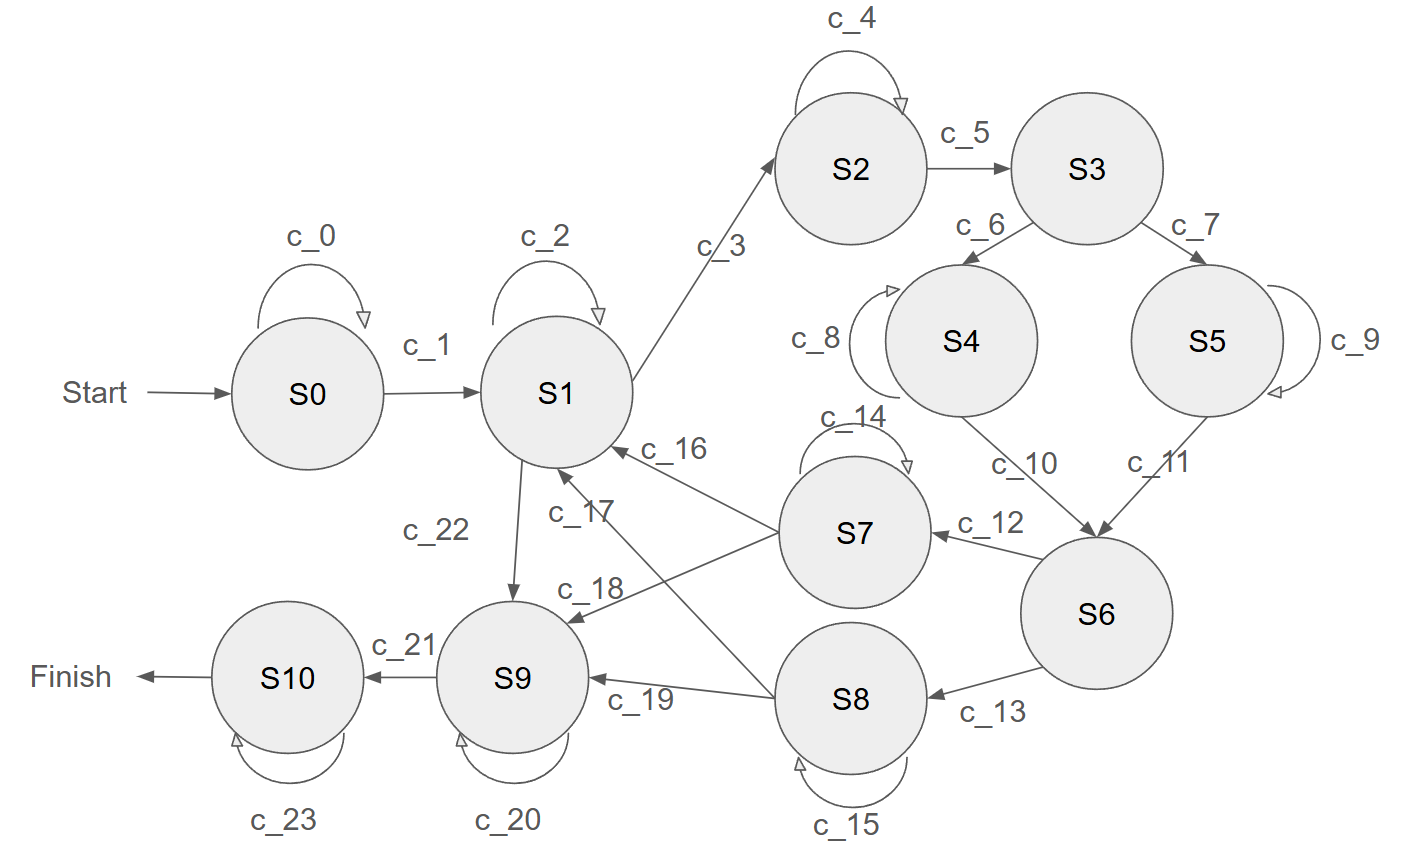
\includegraphics[width=0.8\linewidth]{robot2_fsm.png}
\caption{\label{fig:robot2_fsm}Simulation Environment with the Primary Robot and the Secondary Robot.}
\end{figure}

The conditions for state-transition are shown in Figure~\ref{fig:robot2_fsm} are defined as follows:

\begin{quote}
\begin{description}
    \item[$c_0$] Robot 2 does not move
    \item[$c_1$] Robot 2 moves
    \item[$c_2$] The distance $d_{R_2,o}$ between Robot~2 and an object located on a table 
    at $( -1, -2.8 )\,\text{m}$ or $( 1, -2.8 )\,\text{m}$ satisfies $d_{R_2,o} > 0.2\,\text{m}$
    \item[$c_3$] $d_{R_2,o}$ $ <= 0.2$ m
    \item[$c_4$] Delayed timestep $\tau_\text{delay-pick} < \tau_\text{pick}$
    \item[$c_5$] $\tau_\text{delay-pick} >= \tau_\text{pick}$
    \item[$c_6$] Select Placing Plate 1 and 2
    \item[$c_7$] Select Placing Plate 3 and 4 
    \item[$c_8$] The distance $d_{R_2,p_{12}}$ between Robot 2 and placing plate 1 and 2 on $( 2.8, 1 )\,\text{m}$ $ > 0.35$ m
    \item[$c_9$] The distance $d_{R_2,p_{34}}$ between Robot 2 and placing plate 3 and 4 on $( 2.8, -1 )\,\text{m}$ $ > 0.35$ m
    \item[$c_{10}$] $d_{R_2,p_{12}} <= 0.35$ m
    \item[$c_{11}$] $d_{R_2,p_{34}} <= 0.35$ m
    \item[$c_{12}$] Select a lower layer to place
    \item[$c_{13}$] Select an upper layer to place
    \item[$c_{14}$] Delayed timestep $\tau_\text{delay-place} < \tau_\text{place-l}$
    \item[$c_{15}$] $\tau_\text{delay-place} < \tau_\text{place-u}$
    \item[$c_{16}$] $\tau_\text{delay-place} >= \tau_\text{place-l}$ and an object is on a picking table
    \item[$c_{17}$] $\tau_\text{delay-place} >= \tau_\text{place-u}$ and an object is on a picking table
    \item[$c_{18}$] $\tau_\text{delay-place} >= \tau_\text{place-l}$ and and there is no object on the picking table
    \item[$c_{19}$] $\tau_\text{delay-place} >= \tau_\text{place-u}$ and and there is no object on the picking table
    \item[$c_{20}$] The distance $d_{R_2,op}$ between Robot 2 and the origin position $ > 0.2$ m
    \item[$c_{21}$] $d_{R_2,op} <= 0.2$ m
    \item[$c_{22}$] There is no object on the picking table
    \item[$c_{23}$] Robot 1 is not on $(-1, 0)\,\text{m}$ (the origin position of Robot 1)
\end{description}
\end{quote}

\subparagraph{State Space $\mathcal{S}$}
The state space integrates the instantaneous status of the secondary robot, the relative information of the primary robot and task, and multi-scale historical dynamics. Each component is normalized. The observation vector is defined as:
\[
\mathbf{o}_t = \big[ \mathbf{p}_2, \mathbf{v}_2, \theta_2, \; (\mathbf{p}_{g} - \mathbf{p}_2), d_{g}, \; \mathbf{r}_1, \mathbf{v}_1, \theta_1, \mathbf{v}_{1|2}, v^{rad}_{1|2}, \; \mathbf{s}_{task}, \; \mathbf{c}_{place}, \; \mathbf{h}_t \big],
\]
where
\begin{itemize}
    \item $\mathbf{p}_2 \in \mathbb{R}^2$, $\mathbf{v}_2 \in \mathbb{R}^2$, $\theta_2 \in [-\pi,\pi]$: position, velocity, and orientation (yaw) of the secondary robot,
    \item $\mathbf{p}_{g} \in \mathbb{R}^2$, $d_g \in \mathbb{R}$: relative position and distance to the target,
    \item $\mathbf{r}_1 \in \mathbb{R}^2$, $\mathbf{v}_1 \in \mathbb{R}^2$, $\theta_1 \in [-\pi,\pi]$: relative position, velocity, and orientation of the primary robot,
    \item $\mathbf{v}_{1|2} \in \mathbb{R}^2$, $v^{rad}_{1|2} \in \mathbb{R}$: velocity of Robot~1 relative to Robot~2, and corresponding radial velocity,
    \item $\mathbf{s}_{task} \in \{0,1\}^3$: task status flags, including FSM state index, whether Robot~2 is picking, and whether Robot~1 is carrying,
    \item $\mathbf{c}_{place} \in \{-1,0,1\}^4$: availability of the four placing plates (capability of each plate is 1), with values indicating overfilled ($>1$), occupied ($=1$), or empty($=0$),
    \item $\mathbf{h}_t \in \mathbb{R}^{36}$: multi-scale history features. For horizons $k \in \{5,10,20,50,100,200\}$, we extract
    \[
    \mathbf{h}_{t,k} = \big[ \mathbf{p}_1^{t-k}, \mathbf{p}_2^{t-k}, \Delta d_{1,2}^{t,k}, \tfrac{k}{200} \big],
    \]
    where $\mathbf{p}_1^{t-k}, \mathbf{p}_2^{t-k} \in \mathbb{R}^2$ are past positions of both robots, $\Delta d_{1,2}^{t,k}$ is the change in inter-robot distance since timestep $t-k$, and $\tfrac{k}{200}$ is a normalized time-scale weight.
\end{itemize}

The resulting observation vector is $61$-dimensional:
\[
\mathbf{o}_t \in \mathbb{R}^{61}.
\]

\subparagraph{Action Space $\mathcal{A}$}
The secondary robot executes a set of discrete actions covering navigation, manipulation, and position adjustment. The action space is defined as:
\[
\mathcal{A} = \{a_0, a_1, \dots, a_{9}\}, \quad |\mathcal{A}| = 10 ,
\]
with each action $a_i$ corresponding to:


\begin{itemize}
    \item[$a_0$] \texttt{Brake and do nothing}: Apply braking to Robot 2. This action can be used to maintain the [S0] \texttt{IDLE} state or to prevent collisions with Robot 1.
    \item[$a_1$] \texttt{Navigate to object}: Navigate to a target object on a table at $( -1, -2.8 )\,\text{m}$ or $( 1, -2.8 )\,\text{m}$.
    \item[$a_2$] \texttt{Pick}: Execute the picking operation.
    \item[$a_3$] \texttt{Navigate to plate pair 1/2}: Navigate to $( 2.8, 1 )\,\text{m}$.
    \item[$a_4$] \texttt{Navigate to plate pair 3/4}: Navigate to $( 2.8, -1 )\,\text{m}$.
    \item[$a_5$] \texttt{Place Upper}: Place an object on the upper layer of a plate.
    \item[$a_6$] \texttt{Place Lower}: Place an object on the lower layer of a plate.
    \item[$a_7$] \texttt{Navigate to origin}: Return to the origin position.
    \item[$a_8$] \texttt{Back car}: Set the drive input of Robot 2 to -3, steering to 0, to adjust the position to prevent collisions with Robot 1.
    \item[$a_9$] \texttt{Forward car}: Set the drive input of Robot 2 to 3, steering to 0, to adjust the position to prevent collisions with Robot 1.
\end{itemize}

All navigation actions in this task (e.g., moving to objects or placing plates) follow a consistent policy selection mechanism based on the relative orientation of the target in the robot’s egocentric frame. 
If the target lies within the robot’s forward-facing semicircle (half-plane aligned with the robot’s heading), 
the forward navigation policy $\pi_{\text{nav}}^{f}$ is applied; otherwise, 
the backward navigation policy $\pi_{\text{nav}}^{b}$ is used. 

For pick and place actions (e.g., \texttt{Pick}, \texttt{Place Upper}, or \texttt{Place Lower}), the ideal execution would rely on the policies $\pi_{\text{pick}}$ and $\pi_{\text{place}}$. Since these models are not available, we implement a simulation mechanism to approximate these actions. Specifically, for the pick simulation, we set the maximum pick duration $\tau_\text{pick}$ randomly between 400 and 1000 timesteps and initialize the pick delay counter $\tau_\text{delay-pick}$ to 0. Each timestep during which Robot 2 executes action $a_2$ increments $\tau_\text{delay-pick}$ by 1, when $\tau_\text{delay-pick} >= \tau_\text{pick}$, the object will be moved and fixed on the top of the Chassis of Robot 2, as shown in Figure~\ref{fig:object_on_chassis} . Similarly, for place actions, the ideal execution would rely on the place policy $\pi_{\text{place}}$. In the absence of this model, we simulate the placement process. We set the $\tau_\text{place}$ according to the target layer, lower layer from 200 to 400, upper layer from 600 to 1000, and initialize the placement delay counter $\tau_\text{delay-place}$ to 0. Each timestep during which Robot 2 executes the corresponding place action ($a_5$ for upper-layer placement, $a_6$ for lower-layer placement) increments $\tau_\text{delay-place}$ by 1.

\begin{figure}[H]
\centering
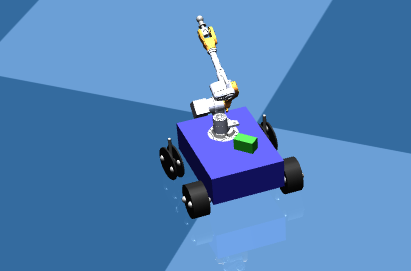
\includegraphics[width=0.5\linewidth]{object_on_chassis.png}
\caption{\label{fig:object_on_chassis}An object is on the top of the Chassis of Robot 2.}
\end{figure}

\subparagraph{Action masking}
To enforce task feasibility and avoid meaningless behaviors, we apply action masking conditioned on the current finite-state-machine (FSM) state $s \in \mathcal{S}_{\text{FSM}}$. The available action set is defined as:
\[
\text{mask}(s) = \{a \in \mathcal{A} \mid a \in \text{ALLOWED\_ACTIONS}[s]\}.
\]

The following table summarizes the set of permissible actions for Robot 2 under each FSM state, using the action symbols defined in Table~\ref{tab:allowed_actions_symbols}.

\begin{table}[H]
\centering
\caption{Allowed actions for each state}
\label{tab:allowed_actions_symbols}
\begin{tabular}{|l|r|}
\hline
\textbf{FSM State} & \textbf{Allowed Actions} \\ \hline
\texttt{[S0] IDLE} & $a_0$; $a_1$ \\ \hline
\texttt{[S1] NAVIGATE\_TO\_PICKING\_POSITION} & $a_0$; $a_1$; $a_9$ \\ \hline
\texttt{[S2] PICKING\_OBJECT} & $a_2$ \\ \hline
\texttt{[S3] MAKE\_DECISION\_ON\_PLACING\_POSITION} & $a_0$; $a_3$; $a_4$ \\ \hline
\texttt{[S4] NAVIGATE\_TO\_PLACING\_POSITION\_1} & $a_0$; $a_3$; $a_8$ \\ \hline
\texttt{[S5] NAVIGATE\_TO\_PLACING\_POSITION\_2} & $a_0$; $a_4$; $a_8$ \\ \hline
\texttt{[S6] MAKE\_DECISION\_ON\_PLACING\_LAYER} & $a_0$; $a_5$; $a_6$ \\ \hline
\texttt{[S7] PLACING\_OBJECT\_UPPER} & $a_5$ \\ \hline
\texttt{[S8] PLACING\_OBJECT\_LOWER} & $a_6$ \\ \hline
\texttt{[S9] MOVING\_TO\_ORIGIN\_POSITION} & $a_0$; $a_7$ \\ \hline
\texttt{[S10] WAIT\_FOR\_FINISH} & $a_0$ \\ \hline
\end{tabular}
\end{table}

\subparagraph{Reward Function}

The reward function $R$ for Robot~2 is implemented as a combination of four components:
\[
R_t = R_\text{time} + R_\text{switch} + R_\text{potential} + R_\text{placement}.
\]

At each timestep, a constant penalty is applied to discourage unnecessarily long episodes:
\[
R_\text{time} = -0.001.
\]

Whenever Robot~2 successfully transitions between FSM states (e.g., from navigation to picking, or from placing to navigating), it receives a positive reward:
\[
R_\text{switch} =
\begin{cases}
+40, & \text{if a valid state transition occurs}, \\
0,   & \text{otherwise}.
\end{cases}
\]

To guide Robot~2 toward its navigation target while avoiding collisions with Robot~1, we use a potential-field formulation.  
Let $\mathbf{p}_2$ and $\mathbf{p}_1 \in \mathbb{R}^2$ denote the positions of Robot~2 and Robot~1, and $\mathbf{p}_t$ the navigation target.  
The attractive potential is
\[
U_{\mathrm{att},t} =
\begin{cases}
\tfrac{1}{2}\|\mathbf{p}_2 - \mathbf{p}_t\|^2, & \text{if target }\mathbf{p}_t \text{ exists}, \\[6pt]
0, & \text{otherwise},
\end{cases}
\]
and the repulsive potential (only active within the influence range $d_\text{inf}=3.0$) is
\[
U_{\mathrm{rep},t} =
\begin{cases}
\left(\tfrac{1}{\|\mathbf{p}_2 - \mathbf{p}_1\|} - \tfrac{1}{d_\text{inf}}\right)^2, & \text{if }\|\mathbf{p}_2-\mathbf{p}_1\| < d_\text{inf}, \\[6pt]
0, & \text{otherwise}.
\end{cases}
\]

The total potential is
\[
U_t = U_{\mathrm{att},t} + U_{\mathrm{rep},t},
\]
and the reward is defined as the potential difference between consecutive steps:
\[
R_{\mathrm{potential},t} =
\begin{cases}
U_{t-1} - U_t, & \text{if previous potential $U_{t-1}$ exists}, \\[4pt]
0, & \text{otherwise}.
\end{cases}
\]

To penalize invalid placements, we impose a penalty proportional to the number of excess objects stacked on each placing plate (capability of each placing plate is 1):
\[
R_\text{placement} = - \sum_{i=1}^N \max(0, \, n_i - 1),
\]
where $n_i$ is the number of objects on plate $i$ and $N$ is the total number of plates.

\paragraph{Training Environment}
We locate the Secondary Robot (Robot 2) at $(-2, 1)\,\text{m}$ to the Simulation Environment with the Primary Robot (Figure~\ref{fig:simenv_with_1st_robot}), the new simulation environment is shown at Figure~\ref{fig:dec_model_inital}. In the new environment, the Primary Robot is still controlled by the Algorithm~\ref{alg:primary_robot_control_logic}.

\begin{figure}[H]
\centering
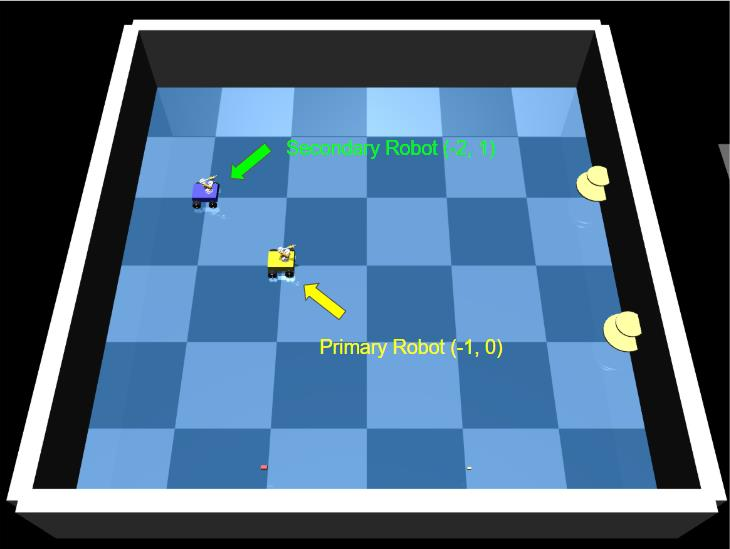
\includegraphics[width=0.8\linewidth]{dec_model_inital.jpeg}
\caption{\label{fig:dec_model_inital}Simulation Environment with the Primary Robot and the Secondary Robot.}
\end{figure}

There are ten objects to be processed via pick-and-place operations. Each placed object is automatically removed from its plate after a delay of 1000–2000 timesteps. The finite state machine (FSM) of Robot~2 is initialized in the \texttt{IDLE} state. To reduce the number of training timesteps, each selected action is repeated for 40 consecutive simulation steps (action repeat).

\subparagraph{Training Configuration}
Hyperparameters used for $\pi_{\text{dec}}$ training are shown as follows:
\begin{itemize}
    \item Environment number: 14
    \item Learning rate: $1 \times 10^{-3}$
    \item Number of steps per environment per update: $n_{\text{steps}} = 2048$
    \item Batch size: $256$
    \item Number of epochs per update: $8$
    \item Entropy coefficient: $\alpha_{\text{ent}} = 0.02$
    \item Value function coefficient: $1.0$
    \item Clipping range: $0.15$
    \item Generalized Advantage Estimation parameter: $\lambda = 0.95$
    \item Total timestamps: $6 \times 10^6$
\end{itemize}

\paragraph{Training Results}

The training results of the $\pi_{\text{dec}}$ are summarized in Figures~\ref{fig:reward_model_curve} and \ref{fig:driver_model_success_curve}. 

Figure~\ref{fig:reward_model_curve} shows the smoothed episode reward curve with a sliding window of 200 episodes. The average reward steadily increases as training progresses, indicating that Robot~2 learns to improve navigation efficiency and reduce collisons.

\begin{figure}[H]
\centering
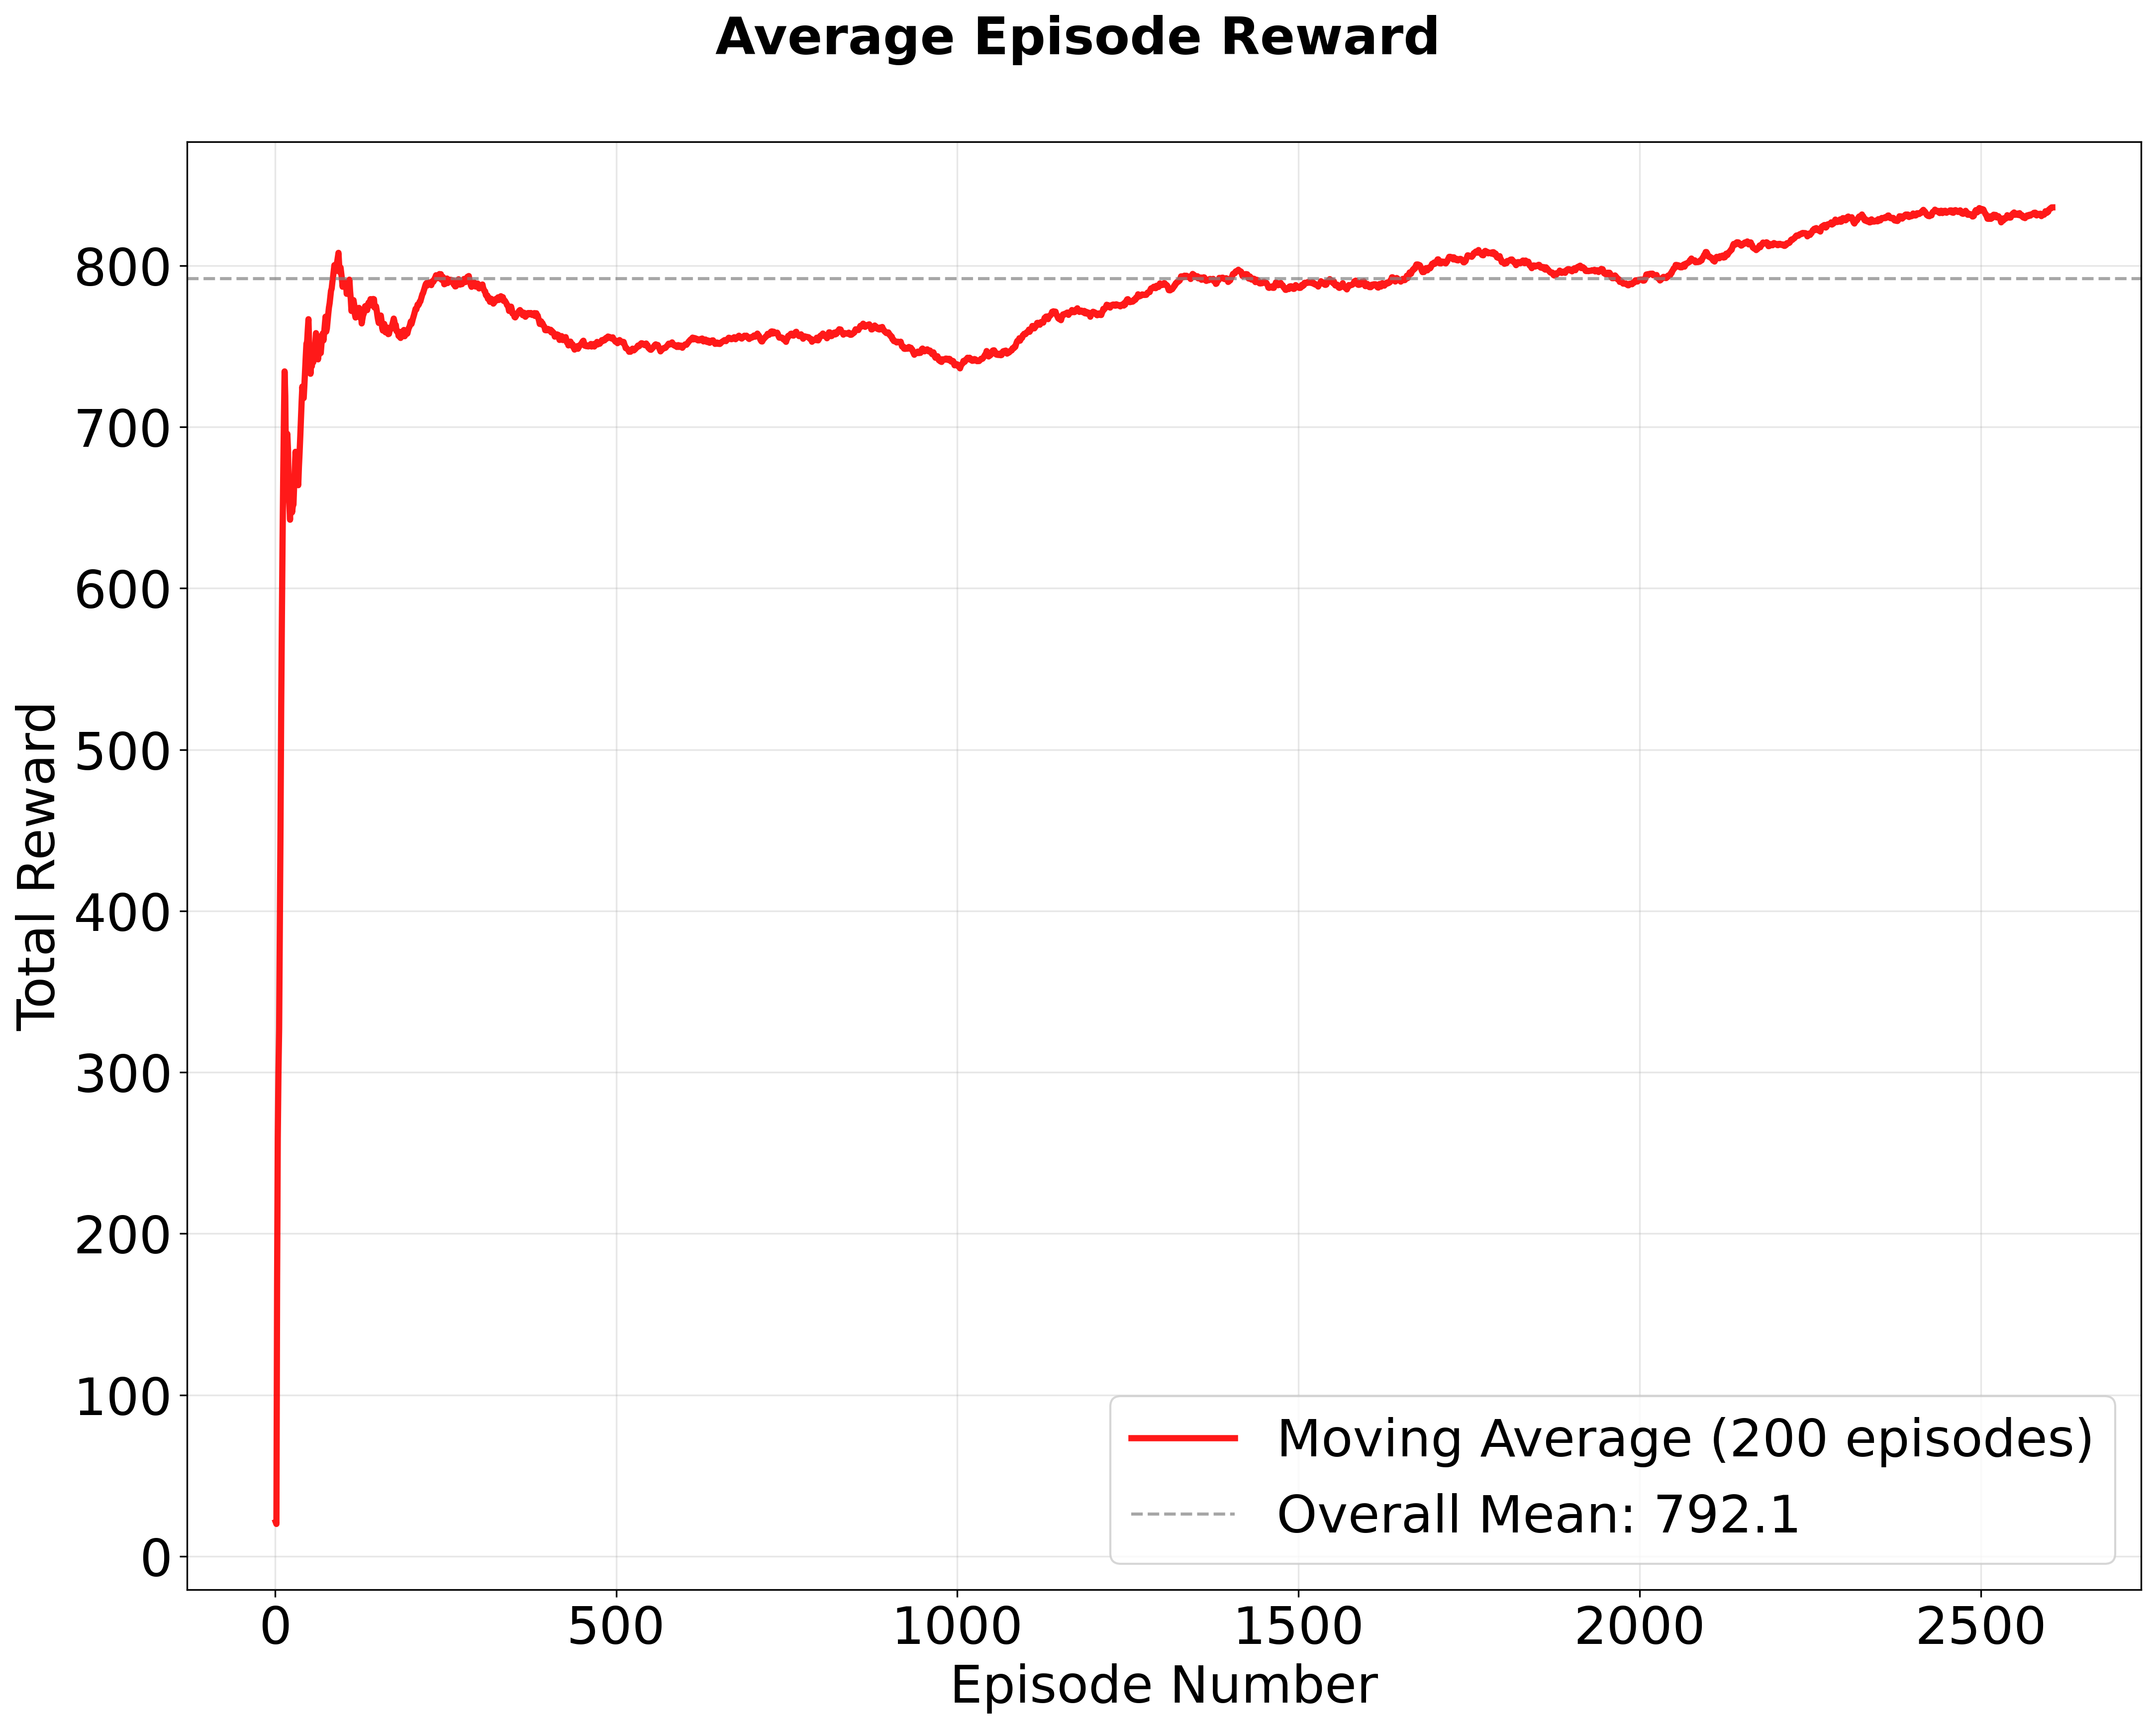
\includegraphics[width=0.5\linewidth]{reward_model_curve.png}
\caption{\label{fig:reward_model_curve}Episode reward curve during training.}
\end{figure}

Figure~\ref{fig:driver_model_success_curve} shows the task success rate, where success is defined as completing all pick-and-place operations without any collisions, measured using a sliding window of 200 episodes. The success rate starts near zero and gradually improves as training progresses. After approximately 2000 episodes, the policy reaches a success rate of around 0.6.

\begin{figure}[H]
\centering
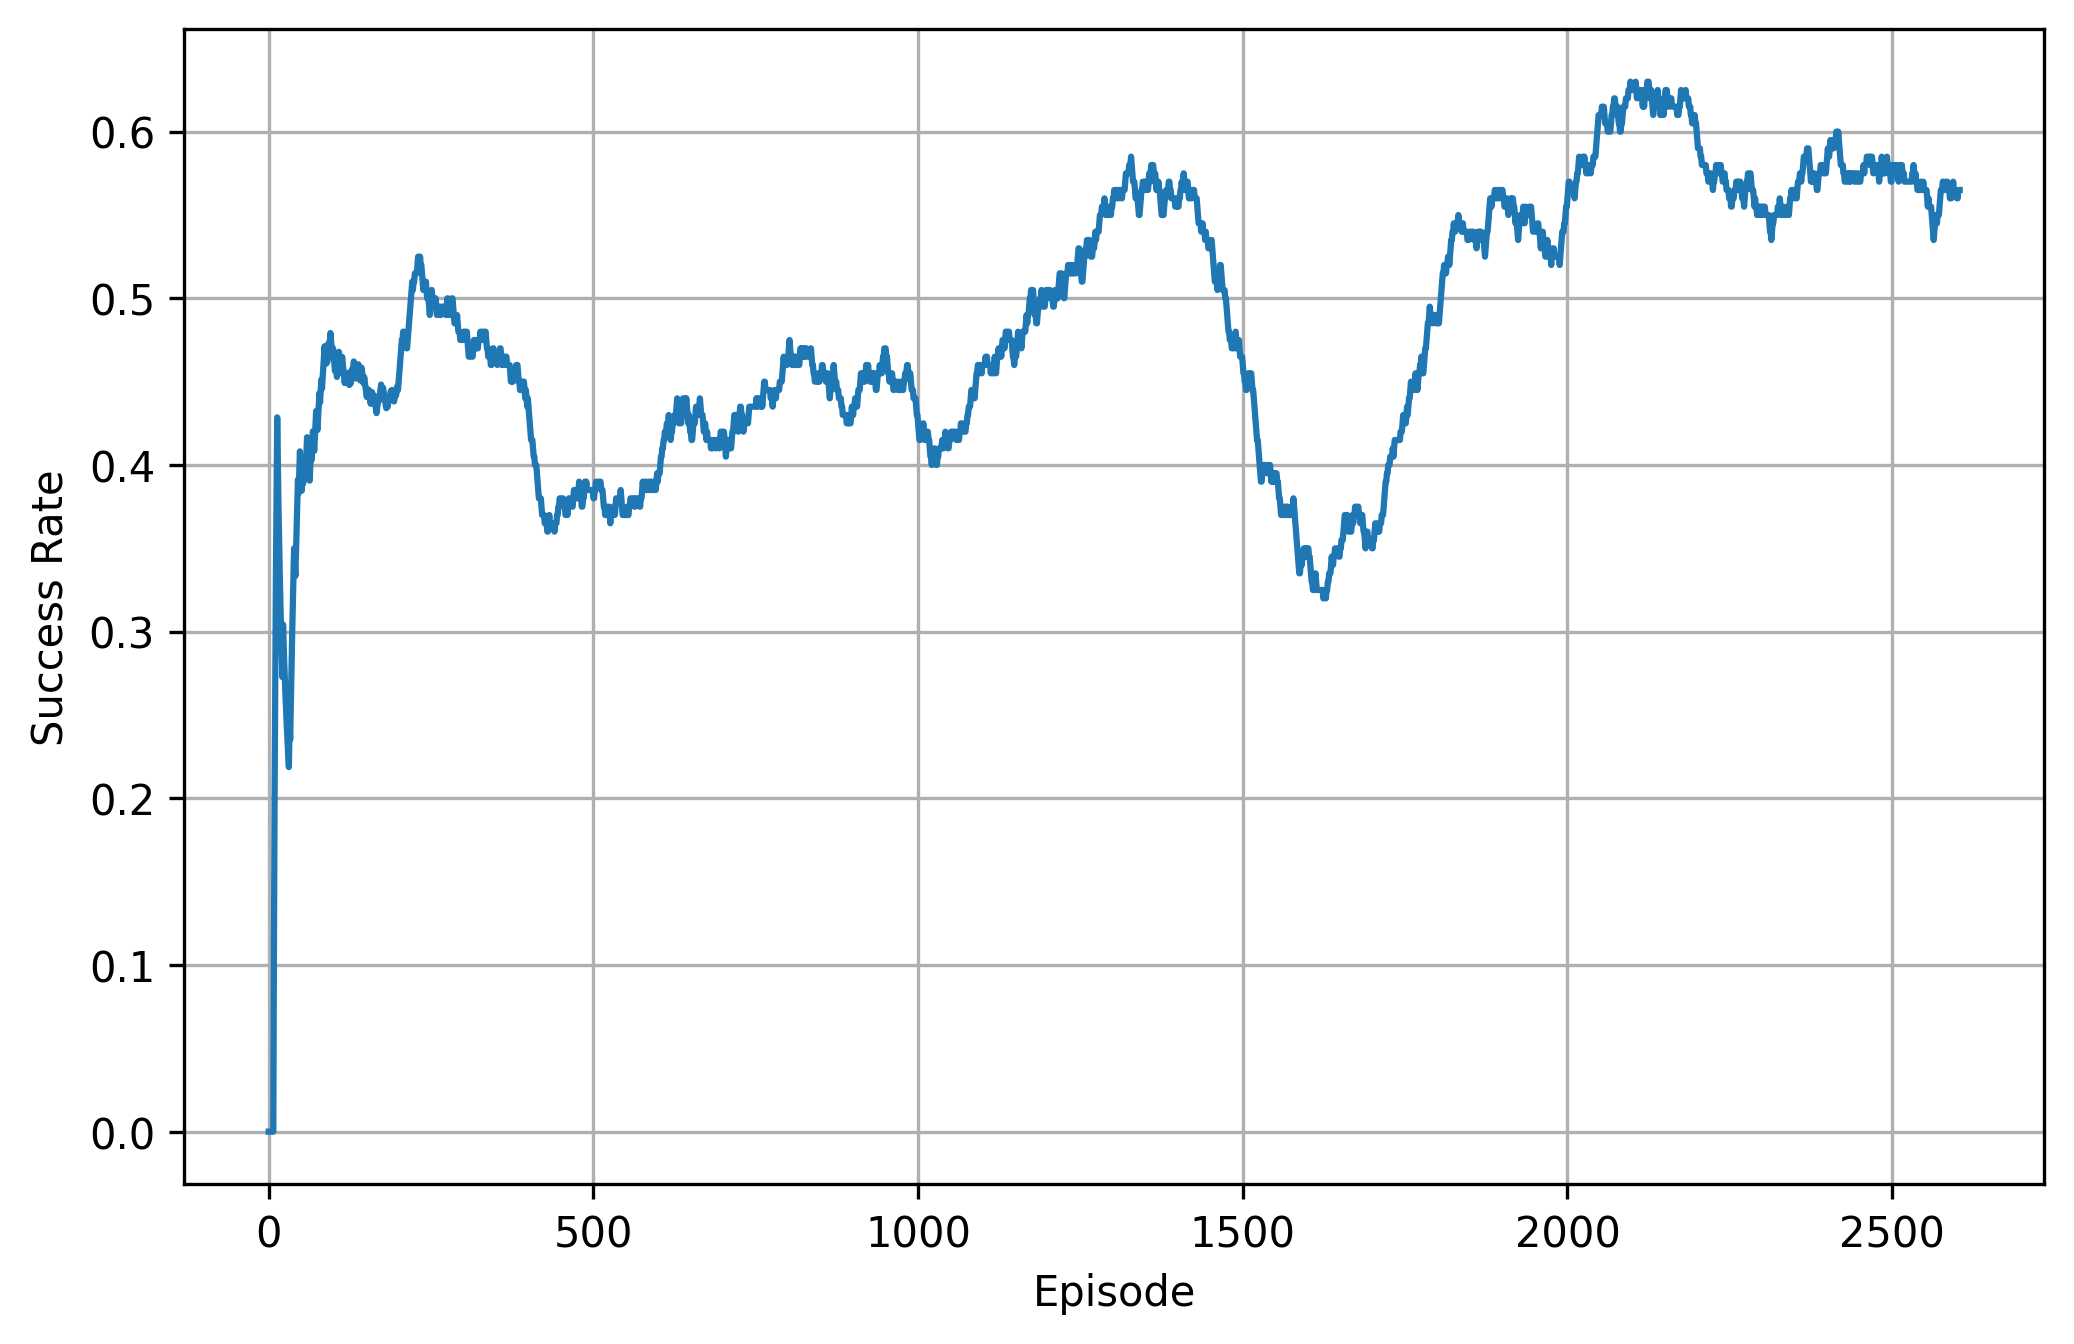
\includegraphics[width=0.75\linewidth]{driver_model_success_curve.png}
\caption{\label{fig:driver_model_success_curve}Task success rate during training with a sliding window of 200 episodes.}
\end{figure}

To further evaluate the robustness of the trained policy $\pi_{\text{dec}}$, we conducted testing over 100 episodes in the same simulation environment. Robot~2 was fully controlled by the trained policy. 

The testing results are summarized as follows:
\begin{itemize}
    \item \textbf{52 episodes (52\%)}: The tasks were successfully completed without any placement penalties or collisions, demonstrating stable and reliable execution.
    \item \textbf{10 episodes (10\%)}: The tasks were completed with placement penalties (multiple objects stacked on a plate), but without any robot–robot collisions. This indicates that while placement constraints were occasionally violated, the robots still managed to finish the pick-and-place operations safely.
    \item \textbf{38 episodes (38\%)}: The tasks failed due to collisions.
\end{itemize}

These results suggest that the trained policy achieves a \textbf{62\% success rate} in completing the task without collisions, and \textbf{52\% fully clean success rate} without either collisions or placement violations.

\section{Case study 2}

In the previous case study, we examined a cooperative scenario involving two robots of identical specifications. In that setting, Robot~1 (R1) was governed by a deterministic control logic, while Robot~2 (R2) was fully controlled by a reinforcement learning (RL) policy. In this section, we extend the study by replacing R1 with another robot with same specifications, denoted as R3, and increasing the complexity of the pick-and-place task. Both R2 and R3 are now controlled by the same newly trained RL model, enabling us to investigate the possibility of collaborative behavior between homogeneous agents. This setup allows us to evaluate not only whether an individual robot can operate independently, but also whether the same learned policy can generalize to collaborative scenarios when multiple agents are present in the environment.

\subsection{Simulation environment}

In this case study, we adopt the same simulation environment introduced in the previous case study, with several modifications to increase the task complexity and enforce stricter placement constraints.  

First, we introduce colors to the objects: each object is either \emph{yellow} or \emph{red}. Correspondingly, the four placing plates are assigned color constraints: plates~1 and~2 are designated as \emph{yellow plates}, which can only accept yellow objects, whereas plates~3 and~4 are designated as \emph{red plates}, which can only accept red objects, as shown in Figure~\ref{fig:red_and_yellow_plates}.  

\begin{figure}[H]
\centering
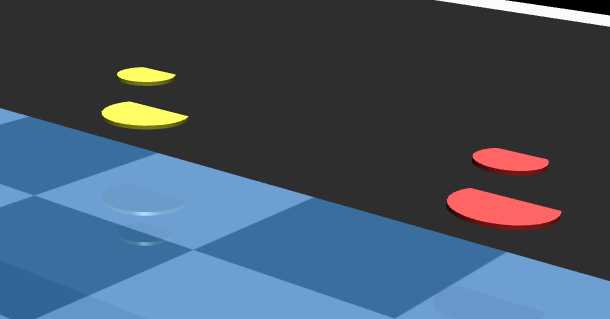
\includegraphics[width=0.75\linewidth]{red_and_yellow_plates.png}
\caption{\label{fig:red_and_yellow_plates}Yellow plates and red plates}
\end{figure}


The total number of objects remains fixed at ten per episode, with a deterministic distribution of \(80\%\) red objects and \(20\%\) yellow objects. Thus, in each independent episode, there are eight red objects and two yellow objects to be processed. While the color distribution is fixed, the order in which objects are placed on the picking table by the placer thread is randomized at the beginning of each episode.

The object will be removed from the plates immediately by the remover thread. 


\subsection{Reinforcement Learning Model Training}

\subparagraph{State Space $\mathcal{S}$}
The state space encodes the instantaneous dynamics of the controlled robot (agent), the relative information of the other robot, task-related signals, and the environment context. Each feature is normalized. The observation vector is defined as:
\[
\mathbf{o}_t = \big[ \mathbf{p}_a, \mathbf{v}_a, \theta_a, f^{pick}_a, f^{place}_a, c_a, m_a, \mathbf{u}_a, \mathbf{p}_o, \mathbf{v}_o, \theta_o, f^{pick}_o, f^{place}_o, c_o, m_o, \mathbf{u}_o, (\mathbf{p}_{g}-\mathbf{p}_a), d_g, f^{g}, \mathbf{c}_{place}, \mathbf{d}_{wall} \big],
\]
where
\begin{itemize}
    \item $\mathbf{p}_a \in \mathbb{R}^2$, $\mathbf{v}_a \in \mathbb{R}^2$, $\theta_a \in [-\pi,\pi]$: position, velocity, and orientation (yaw) of the agent robot,
    \item $f^{pick}_a, f^{place}_a \in \{0,1\}$: binary flags indicating whether the agent robot can pick or place,
    \item $c_a \in \{0,1\}$: whether the agent robot is carrying an object,
    \item $m_a \in \{-1,0,1\}$: color of the carried object (\(-1\): none, \(0\): yellow, \(1\): red),
    \item $\mathbf{u}_a \in \{0,1\}^3$: agent’s manipulation status (currently picking, placing, placing-upper, placing-lower),
    \item $\mathbf{p}_o \in \mathbb{R}^2$, $\mathbf{v}_o \in \mathbb{R}^2$, $\theta_o \in [-\pi,\pi]$: position, velocity, and orientation of the other robot,
    \item $f^{pick}_o, f^{place}_o \in \{0,1\}$: binary flags for whether the other robot can pick or place,
    \item $c_o \in \{0,1\}$: whether the other robot is carrying an object,
    \item $m_o \in \{-1,0,1\}$: color of the object carried by the other robot,
    \item $\mathbf{u}_o \in \{0,1\}^3$: other robot’s manipulation status (picking, placing, placing-upper, placing-lower),
    \item $(\mathbf{p}_{g}-\mathbf{p}_a) \in \mathbb{R}^2$, $d_g \in \mathbb{R}$: relative position and distance from the agent robot to the current target,
    \item $f^{g} \in \{0,1\}$: whether a valid target is assigned,
    \item $\mathbf{c}_{place} \in \{-1,0,1\}^4$: states of the four placing plates ($0$: empty, $1$: one object placed, $-1$: capacity exceeded),
    \item $\mathbf{d}_{wall} \in \mathbb{R}^4$: normalized distances from the agent robot to the four walls.
\end{itemize}

\subparagraph{Action Space $\mathcal{A}$}
The action space is defined as a discrete set
\[
\mathcal{A} = \{a_{\text{i}}, a_{\text{f}}, a_{\text{b}}, a_{\text{l}}, a_{\text{r}}, a_{\text{pk}}, a_{\text{pu}}, a_{\text{pl}}\},
\]
where each action corresponds to a primitive operation of the agent robot:
\begin{align*}
a_{\text{i}} &: \text{no-op (idle)}, \\
a_{\text{f}} &: \text{move forward, increasing the robot position by } (0.05, 0), \\
a_{\text{b}} &: \text{move backward, decreasing the robot position by } (0.05, 0), \\
a_{\text{l}} &: \text{move left, increasing the robot position by } (0, 0.05), \\
a_{\text{r}} &: \text{move right, decreasing the robot position by } (0, 0.05), \\
a_{\text{pk}} &: \text{move an object from the table onto the Chassis of the robot without any delay}, \\
a_{\text{pu}} &: \text{place the carried object onto the nearest upper plate without any delay}, \\
a_{\text{pl}} &: \text{place the carried object onto the nearest lower plate without any delay}.
\end{align*}

\subparagraph{Action validity}
Invalid actions are filtered by a rule-based feasibility check instead of applying action masking.  
Let $\mathcal{V}_{\text{rule}}(s_t) \subseteq \{a_{\text{i}}, a_{\text{f}}, a_{\text{b}}, a_{\text{l}}, a_{\text{r}}, a_{\text{pk}}, a_{\text{pu}}, a_{\text{pl}}\}$ denote the set of feasible actions at state $s_t$.  
The validity conditions for the actions are defined as follows:

\begin{itemize}
    \item \textbf{Navigation lock.}  
    Navigation actions $a_{\text{f}},a_{\text{b}},a_{\text{l}},a_{\text{r}}$ are invalid if the agent is currently in a picking or placing phase.

    \item \textbf{Pick constraints.}  
    The pick action $a_{\text{pk}}$ is valid only if the agent is not already carrying an object and there exists an object within a distance $d \leq 0.5$.

    \item \textbf{Place constraints.}  
    The place actions $a_{\text{pu}}, a_{\text{pl}}$ are valid only if the agent is carrying an object and is within the threshold distance $\tau_j$ of a valid placing plate $j$, with  
    \[
    \tau_j = 
    \begin{cases}
        1.0 & \text{if plate } j \text{ is a yellow plate}, \\
        0.5 & \text{if plate } j \text{ is a red plate}.
    \end{cases}
    \]

    \item \textbf{Color–plate consistency.}  
    If the carried object has color $c \in \{\text{RED}, \text{YELLOW}\}$, then placement is only valid when the agent is near a plate of matching color; otherwise $a_{\text{pu}}$ and $a_{\text{pl}}$ are invalid.
\end{itemize}

\subparagraph{Invalid action handling}  
The executed action $\hat{a}_t$ is then given by
\[
\hat{a}_t =
\begin{cases}
a_t, & \text{if } a_t \in \mathcal{V}_{\text{rule}}(s_t), \\
a_{\text{i}}, & \text{otherwise}.
\end{cases}
\]

\subparagraph{Reward function}  
Let $r_t$ denote the reward received by the agent at timestep $t$. It is composed of multiple components:  

\[
r_t = r_{\text{step}} + r_{\text{action}} + r_{\text{potential}} + r_{\text{collision}} + r_{\text{task}}
\]

where

1. \textbf{Step penalty} (to encourage efficiency):
\[
r_{\text{step}} = -0.001
\]

2. \textbf{Action reward}:
\[
r_{\text{action}} =
\begin{cases}
20, & \text{if } a_t \in \{a_{\text{pk}}, a_{\text{pu}}, a_{\text{pl}}\}, \\
0, & \text{otherwise}.
\end{cases}
\]

3. \textbf{Potential field reward} (encouraging progress toward target and avoiding the other robot):  

Let $\mathbf{p}_t$ be the agent robot's current position, $\mathbf{p}_{\text{target}}$ the target position, and $\mathbf{p}_{\text{other}}$ the other robot's position. Define attractive and repulsive potentials:

\[
U_{\text{attr}} = \frac{1}{2} \|\mathbf{p}_t - \mathbf{p}_{\text{target}}\|^2, 
\quad 
U_{\text{rep}} =
\begin{cases}
\left(\frac{1}{\|\mathbf{p}_t - \mathbf{p}_{\text{other}}\|} - \frac{1}{d_{\text{influence}}}\right)^2, & \|\mathbf{p}_t - \mathbf{p}_{\text{other}}\| < d_{\text{influence}}, \\
0, & \text{otherwise},
\end{cases}
\]

with $d_{\text{influence}} = 1.0$. Then the potential field reward is

\[
r_{\text{potential}} = U_{\text{prev}} - (U_{\text{attr}} + U_{\text{rep}}),
\]

where $U_{\text{prev}}$ is the potential at the previous timestep (encouraging the agent to reduce potential).

4. \textbf{Collision penalties}:
\[
r_{\text{collision}} = 
\begin{cases}
-10, & \text{if collision with robot or forbidden area occurs}, \\
0, & \text{otherwise}.
\end{cases}
\]

5. \textbf{Task completion reward}:
\[
r_{\text{task}} = 
\begin{cases}
+60, & \text{if task completed successfully}, \\
0, & \text{otherwise}.
\end{cases}
\]

An episode terminates when any of the following conditions occur:

\begin{itemize}
    \item \textbf{Collision termination:}  
    The episode ends immediately if the agent robot collides with the other robot or any forbidden area.

    \item \textbf{Task completion:}  
    The episode ends if the task is completed (all of the objects are removed from the plates).

    \item \textbf{Maximum steps:}  
    The episode ends if the step limit of 8000 is reached.
\end{itemize}

\paragraph{Training Environment}  
The training environment is initialized with Robot2 (white) placed at position $(-2, -1)$ m and Robot3 (purple) at position $(-2, 1)$ m, as shown in Figure~\ref{fig:case_2_training_env}.  

\begin{figure}[H]
\centering
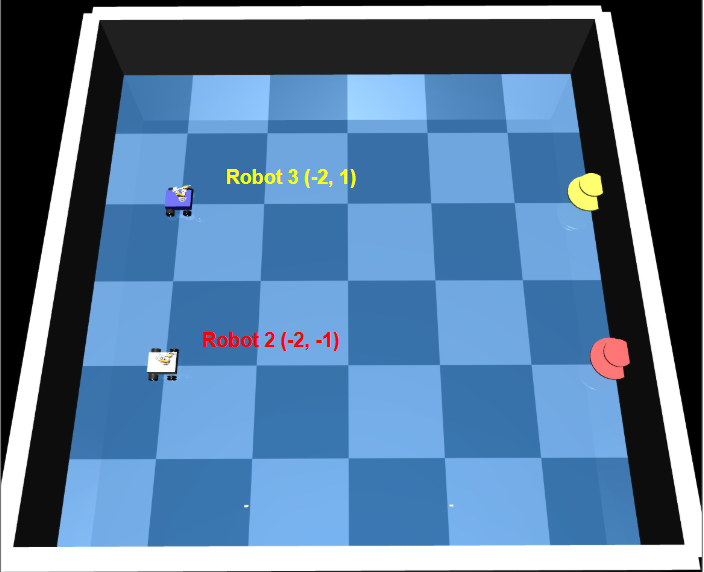
\includegraphics[width=0.75\linewidth]{case_2_training_env.png}
\caption{\label{fig:case_2_training_env}Initial positions of Robot~2 and Robot~3.}
\end{figure}

We adopt a multi-round alternating training scheme over 9 rounds to obtain a single policy capable of independently controlling both robots while avoiding inter-robot and walls collisions.

In the first training round, one robot is randomly assigned to the agent for training, while the other robot remains stationary. This yields the initial policy $\pi_1$.  

For subsequent rounds, we employ an alternating training procedure. Specifically, in round $k$ ($2 \le k \le 9$), the agent trains one robot based on the policy $\pi_{k-1}$, while the other robot is controlled by the previously learned policy $\pi_{k-1}$. The resulting policy after round $k$ is denoted as $\pi_k$.

This process is repeated until the ninth round, producing the final policy $\pi_9$.

Each training round is conducted using a parallel environment setup with $N=14$ independent instances. The agent is trained with the Proximal Policy Optimization (PPO) algorithm using a multi-layer perceptron (MLP) policy. The hyperparameters are set as follows:

\begin{itemize}
    \item Learning rate: $1 \times 10^{-3}$
    \item Entropy coefficient: $\alpha_{\text{ent}} = 0.02$
    \item Number of steps per environment update: $n_{\text{steps}} = 2048$
    \item Batch size: $256$
    \item Number of epochs per update: $8$
    \item Value function coefficient: $1.0$
    \item Clipping parameter: $0.15$
    \item GAE $\lambda$: $0.95$
    \item Total timestamps: $12 \times 10^6$
\end{itemize}

\paragraph{Training Results}  

The training results are presented in two parts.  

\textbf{Reward curves.} The first part consists of the reward curves obtained over the nine rounds of alternating training. These curves illustrate the progression of learning and convergence of the policy over successive training rounds, as shown in Figure~\ref{fig:reward_curves_9rounds}.  

\begin{figure}[H]
\centering

\includegraphics[width=0.9\linewidth]{reward_curves_9rounds.png}
\caption{\label{fig:reward_curves_9rounds}Reward curves of 9 rounds}
\end{figure}

\textbf{Evaluation metrics.} The second part focuses on evaluating the performance of the trained policies. In the testing phase, both robots are controlled independently by the latest policy obtained from each training round. For each policy, we conduct 100 evaluation episodes to ensure statistical reliability, and the deterministic policy
set to False. We define six evaluation metrics:


\begin{enumerate}
    \item \textbf{Average progress.} This metric quantifies the number of objects successfully placed by the robots before encountering an environment collision, a robot-robot collision, or completing the task. The value ranges from 0 to 10 and measures the efficiency of the policy when controlling both robots independently, as shown in Figure~\ref{fig:progress_completion_per_policy}.  

    \item \textbf{Task completion rate.} Defined as the proportion of episodes in which the robots successfully complete the task, this metric evaluates the overall success of the policy under full multi-agent control, as shown in Figure~\ref{fig:progress_completion_per_policy}. 

    \begin{figure}[H]
    \centering
    
\includegraphics[width=0.9\linewidth]{progress_completion_per_policy.png}
    \caption{\label{fig:progress_completion_per_policy}Average progress and task completion rate of 9 policies}
    \end{figure}

    \item \textbf{Timesteps per placed object.} This metric evaluates the efficiency of object placement under multi-agent control by quantifying the average number of simulation steps required to successfully place a single object. It is formally defined as
    \[
    \text{Timesteps per Placed Object} = \frac{\sum \text{Timesteps}}{\sum \text{Placed Objects}},
    \]
    where the sums are taken over episodes in which at least one object is placed (episodes with zero placements are excluded). A lower value of this metric indicates that, on average, fewer timesteps are needed per object, reflecting more efficient coordination and faster task execution by the two robots, as shown in Figure~\ref{fig:timesteps_per_object}. 

    \begin{figure}[H]
    \centering
    
\includegraphics[width=0.9\linewidth]{timesteps_per_object.png}
    \caption{\label{fig:timesteps_per_object}Curve of Timesteps per placed object.}
    \end{figure}
 

    \item \textbf{Independent-agent Average Progress.} To evaluate the policy's ability to make progress when controlling a single robot independently, we perform additional tests in which, for each episode, one robot is randomly selected to be controlled by the policy while the other robot remains stationary. For each policy $\pi_k$, 100 episodes of independent-agent testing are conducted. The Average Progress is calculated as the number of objects successfully placed by the controlled robot before the episode ends due to collision or task completion, as shown in Figure~\ref{fig:ind_progress_completion_per_policy}.  

    \item \textbf{Independent-agent Task Completion Rate.} Under the same independent-agent testing setup, we measure the proportion of episodes in which the controlled robot successfully completes the task. This metric provides insight into the policy's ability to achieve the goal when controlling a single robot in isolation, as shown in Figure~\ref{fig:ind_progress_completion_per_policy}.

    \begin{figure}[H]
    \centering
    
\includegraphics[width=0.9\linewidth]{ind_progress_completion_per_policy.png}
    \caption{\label{fig:ind_progress_completion_per_policy}Independent-agent average progress and task completion rate of 9 policies.}
    \end{figure}
    
    \item \textbf{Independent-agent Timesteps per Placed Object.} Using the same independent-agent tests, this metric measures the efficiency of object placement, as shown in Figure~\ref{fig:independent_agent_timesteps_per_object}. 

    \begin{figure}[H]
    \centering
    
\includegraphics[width=0.9\linewidth]{independent_agent_timesteps_per_object.png}
    \caption{\label{fig:independent_agent_timesteps_per_object}Independent-agent Curve of Timesteps per placed object.}
    \end{figure}



\end{enumerate}



% We hope you find Overleaf useful, and do take a look at our \href{https://www.overleaf.com/learn}{help library} for more tutorials and user guides! Please also let us know if you have any feedback using the \textbf{Contact us} link at the bottom of the Overleaf menu --- or use the contact form at \url{https://www.overleaf.com/contact}.

\bibliographystyle{IEEEtran}
\bibliography{reference}

\end{document}
